\documentclass[a4paper,12pt]{article}

% Pacchetti per la codifica e la lingua
\usepackage[utf8]{inputenc}
\usepackage[T1]{fontenc}
\usepackage[italian]{babel}

% Pacchetti per la formattazione
\usepackage{geometry}
\geometry{a4paper, margin=2.5cm}
\usepackage{graphicx}
\usepackage{float}
\usepackage{booktabs} % Per tabelle più belle
\usepackage{array}    % Per gestire la larghezza delle colonne nelle tabelle
\usepackage{hyperref} % Per i link
\usepackage{amsmath}  % Per simboli matematici

% Impostazioni link
\hypersetup{
    colorlinks=true,
    linkcolor=black,
    filecolor=magenta,      
    urlcolor=blue,
}

\usepackage[
    backend=biber,             
    style=ieee,               
    sorting=none         
]{biblatex}

\addbibresource{bibliography.bib} 

\begin{document}

\begin{titlepage}
\begin{center}
    
\includegraphics[width=0.25\textwidth]{img/logo_università.png} \\[1.5cm]

    {\Large \textbf{Alma Mater Studiorum - Università di Bologna}}\\[0.3cm]
    {\large Corso di Laurea Magistrale in Informatica}\\[0.5cm]

    {\large Corso di Intelligenza Artificiale}\\[2cm]

    {\LARGE \textbf{Relazione Progetto 6: Valutazione e Fine-Tuning di Modelli Linguistici (LLM)}}\\[2cm]

    {\large
    Alexandru Bogdan Nicolescu \\
    Pietro Cimino \\
    Mattia Boffa \\
    Alessandro Modelli
    }\\[2cm]

    {\large Marzo 2026}\\[0.5cm]
    \vfill
\end{center}
\end{titlepage}

\section{Introduzione}

\subsection{Descrizione del Problema}
Il \textbf{Progetto 6: Valutazione e Fine-Tuning di Modelli Linguistici (LLM)} ha come obiettivo principale l'analisi comparativa
di modelli linguistici pre-addestrati, valutandone le capacità di adattamento a task specifici. Il focus del lavoro risiede
nell'esecuzione pratica di diverse strategie di \textbf{Fine-Tuning} su modelli distinti, al fine di misurarne quantitativamente
le prestazioni post-adattamento e farne emergere, tramite confronto diretto, i rispettivi \textbf{punti di forza e di debolezza}.

Nello specifico, il nostro gruppo ha selezionato il task di \textbf{Emotion Recognition} (Classificazione delle Emozioni) applicato
a testi brevi provenienti dai social media. La rilevanza di questo problema è elevata nell'attuale panorama digitale: la capacità
di analizzare automaticamente il ``sentiment'' e le sfumature emotive (gioia, tristezza, rabbia, ecc.) su piattaforme come Twitter
è cruciale per applicazioni di monitoraggio della brand reputation, analisi sociale e customer care automatizzato.

Il pubblico di riferimento include ricercatori NLP, data scientist e sviluppatori di assistenti virtuali empatici. Una soluzione
efficace permette di automatizzare l'analisi di grandi moli di dati non strutturati (Big Data) con costi ridotti rispetto
all'annotazione manuale.

\subsection{Soluzione Proposta}
Per affrontare il problema, abbiamo adottato un \textbf{approccio sperimentale comparativo}, testando diverse tecniche di
fine-tuning su una selezione eterogenea di modelli pre-addestrati. L'obiettivo centrale è stato confrontare l'efficacia delle
diverse strategie di adattamento in relazione alle architetture sottostanti in riferimento al Dataset scelto:

\begin{itemize}
    \item {\textbf{Emotion di Hugging Face:} pubblicato da dair-ai, è una raccolta di messaggi di Twitter in inglese annotati con sei emozioni di base: sadness (tristezza), joy (gioia), love (amore), anger (rabbia), fear (paura) e surprise (sorpresa), pensato per compiti di text classification multiclassificazione e ricerca nel riconoscimento delle emozioni nel testo.
          I dati sono suddivisi nei classici split train, validation e test. Una caratteristica importante evidenziabile dai grafici, è che la distribuzione delle classi non è bilanciata: alcune emozioni (come sadness e joy) tendono ad essere molto più rappresentate rispetto ad altre (come surprise o love), soprattutto nel training set. Questo sbilanciamento può influenzare l’addestramento dei modelli perché le classi maggioritarie dominano l’apprendimento, mentre quelle minoritarie rischiano di essere trascurate.}

          \begin{center}
              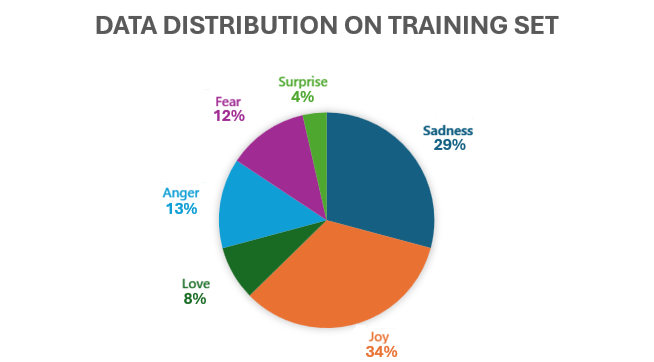
\includegraphics[width=0.7\textwidth]{img/immagine1.png}\\[1.5cm]
              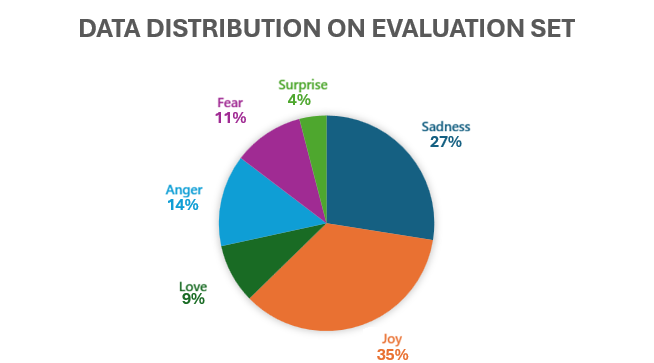
\includegraphics[width=0.7\textwidth]{img/immagine2.png}\\[1.5cm]
              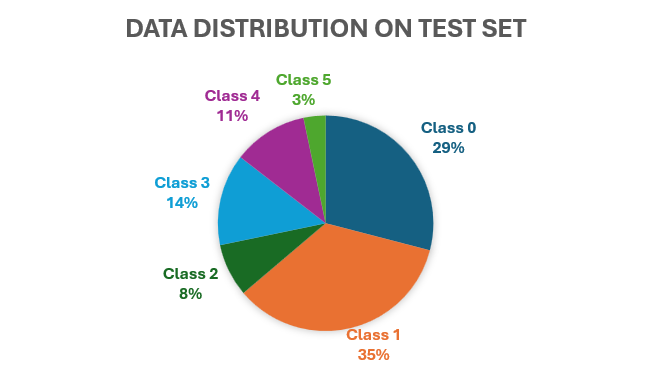
\includegraphics[width=0.7\textwidth]{img/immagine3.png}
          \end{center}
\end{itemize}

La nostra soluzione si articola nei seguenti punti:

\begin{itemize}
    \item \textbf{Modelli Selezionati:} Abbiamo condotto esperimenti su quattro architetture distinte per valutare l'impatto della
          dimensione e della specializzazione del pre-training:
          \begin{itemize}
              \item \texttt{vinai/bertweet-base}: Modello domain-specific per Twitter.
              \item \texttt{distilbert/distilbert-base-uncased}: Modello distillato (leggero) per testare l'efficienza.
              \item \texttt{google-bert/bert-base-uncased}: La baseline standard per il NLP.
              \item \texttt{FacebookAI/roberta-base}: Versione ottimizzata di BERT.
          \end{itemize}

    \item \textbf{Approccio Metodologico:} Un confronto sistematico tra diverse metodologie di apprendimento:
          \begin{enumerate}
              \item \textbf{In-Context Learning:} In seguito all’addestramento del solo classificatore mantenendo il corpo del modello congelato (Alignment classification head), si è utilizzato il metodo di prompt engineering few-shot con diversi gradi.

              \item \textbf{Complete Fine-Tuning:} Aggiornamento di tutti i pesi del modello per l’adattamento al task.
          \end{enumerate}

    \item \textbf{Sfide Computazionali:} Le principali difficoltà affrontate sono state la gestione della \textbf{Context Window}
          limitata (tipica dei modelli Encoder-Only), che ha imposto vincoli severi sulle strategie di Few-Shot Learning, e la sfida di
          massimizzare le performance di generalizzazione nonostante il \textbf{basso numero di parametri} dei modelli ``base'' e
          ``distilled'' selezionati, richiedendo un'ottimizzazione fine degli iperparametri. Un'ulteriore sfida è rappresentata dallo
          \textbf{sbilanciamento delle classi} nel dataset: come evidenziato in Figura \ref{fig:class_distribution}, le classi
          \textit{Joy} e \textit{Sadness} dominano il training set (rispettivamente $\sim$5300 e $\sim$4700 campioni), mentre
          \textit{Surprise} conta appena $\sim$600 esempi, rendendo più difficile la generalizzazione sulle emozioni minoritarie.

          \begin{figure}[H]
              \centering
              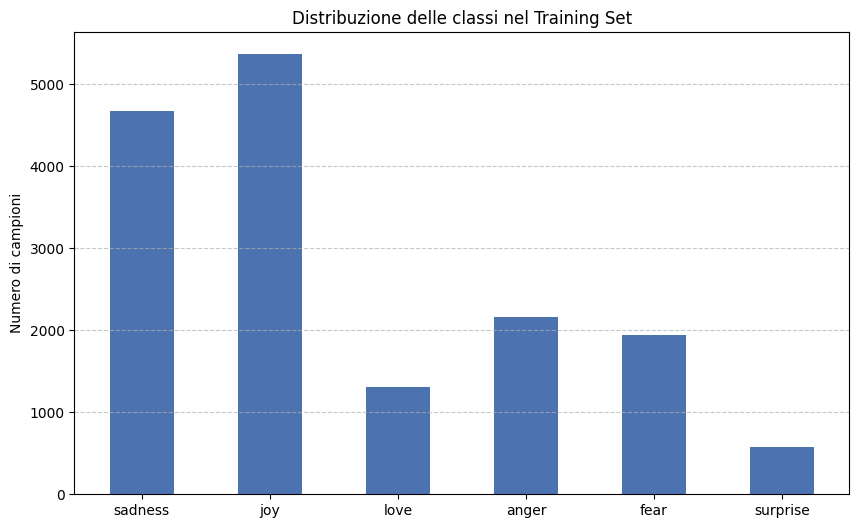
\includegraphics[width=0.75\textwidth]{img/class_distribution.png}
              \caption{Distribuzione delle classi nel Training Set: evidente sbilanciamento tra \textit{Joy}/\textit{Sadness} e \textit{Surprise}.}
              \label{fig:class_distribution}
          \end{figure}
\end{itemize}

\paragraph{Distribuzione dei Compiti:}
Il lavoro è stato parallelizzato assegnando a ciascun membro del gruppo la responsabilità completa di una specifica architettura.
Ogni componente ha curato l'analisi esplorativa, il pre-processing, il fine-tuning e la valutazione del proprio modello, per poi
convergere in una fase finale di confronto dei risultati.

\begin{itemize}
    \item \textbf{[Alexandru Bogdan Nicolescu]:} Responsabile per \texttt{vinai/bertweet-base}.
    \item \textbf{[Pietro Cimino]:} Responsabile per \texttt{distilbert/distilbert-base-uncased}.
    \item \textbf{[Mattia Boffa]:} Responsabile per \texttt{google-bert/bert-base-uncased}.
    \item \textbf{[Alessandro Modelli]:} Responsabile per \texttt{FacebookAI/roberta-base}.
\end{itemize}

\subsection{[extra] Revisione della Letteratura}
In letteratura, il benchmark per il riconoscimento delle emozioni su testo fa spesso riferimento al
dataset \texttt{dair-ai/emotion}, introdotto originariamente da Saravia et al. (2018)\cite{saravia-etal-2018-carer} nel
lavoro ``CARER: Contextualized Affect Representations for Emotion Recognition''.
Questo dataset è stato costruito utilizzando hashtag come etichette deboli (distant supervision)
per classificare i tweet in categorie emotive fondamentali.

Per quanto riguarda i modelli, lo stato dell'arte su dati provenienti da Twitter è rappresentato da
architetture domain-specific come \texttt{BERTweet}, presentato da Nguyen et al. (2020) \cite{nguyen-etal-2020-bertweet}.
\texttt{BERTweet} utilizza la stessa architettura di BERT-base ma è stato
pre-addestrato su un corpus massivo di 850 milioni di tweet inglesi, dimostrando prestazioni superiori
rispetto a RoBERTa e XLM-R su task di classificazione testuale, POS tagging e NER in ambito social
media.

Tuttavia, approcci di Full Fine-Tuning su questi modelli richiedono risorse computazionali significative.
Per mitigare questo problema, Hu et al. (2021) \cite{LoRA} hanno proposto \textbf{LoRA (Low-Rank Adaptation)}. Questa tecnica congela i pesi del modello pre-addestrato e inietta matrici di
decomposizione di rango ridotto nei layer del Transformer, riducendo drasticamente il numero di parametri
addestrabili (fino a 10.000 volte in meno rispetto al fine-tuning completo su GPT-3) senza introdurre
latenza in inferenza. Il nostro lavoro dimostra come l'applicazione di LoRA su BERTweet,
se ben calibrata, possa eguagliare i metodi tradizionali a una frazione del costo computazionale.

\section{Metodo Proposto}

\subsection{Scelta della Soluzione}
Abbiamo scartato l'uso di LLM generativi generalisti (es. GPT-4, Llama-3) per motivi di latenza in inferenza e costi computazionali, preferendo architetture \textbf{Encoder-Only} (come \texttt{BERTweet} e le varianti di \texttt{BERT}/\texttt{RoBERTa}). I modelli Encoder sono strutturalmente superiori nei task di classificazione pura grazie all'attenzione bidirezionale che cattura l'intero contesto della frase simultaneamente.

Inizialmente è stato eseguito un addestramento del solo classification
head che pur essendo computazionalmente leggero e veloce presenta lo svantaggio di
congelare il corpo del modello, limitandone drasticamente la capacità di apprendimento
su domini complessi al fine di testare la tecnica di In-Context Learning per
testare le capacità native (\textit{zero-shot} e \textit{few-shot}) dei
modelli senza effettuare alcun aggiornamento dei pesi, scontrandoci tuttavia con i severi limiti imposti dalla context window
ristretta tipica di queste architetture.
Successivamente, abbiamo testato il Complete Fine-Tuning, il quale aggiorna la
totalità dei pesi garantendo un’ottima accuratezza, ma risultando al contempo lento
e molto oneroso in termini di memoria.


\subsection{Metodologia per la misurazione delle prestazioni}
Le prestazioni sono state valutate utilizzando un set di metriche standard per la classificazione multiclasse, selezionate per fornire una visione sia quantitativa che qualitativa:

\begin{itemize}
    \item \textbf{Accuracy:} Rappresenta la frazione di predizioni corrette rispetto al totale dei campioni. Sebbene sia la metrica più intuitiva per una valutazione globale, in questo progetto viene utilizzata solo come riferimento di base, poiché può risultare ingannevole in presenza di dataset sbilanciati (un modello che predice sempre la classe maggioritaria avrebbe comunque un'accuratezza elevata).

    \item \textbf{F1-Score:} È la media armonica tra \textit{Precision} e \textit{Recall}, calcolata indipendentemente per ogni classe e poi mediata (senza pesare per la numerosità delle istanze). Questa è la metrica \textbf{critica} per il nostro task a causa del forte sbilanciamento del dataset (le classi \textit{Joy} e \textit{Sadness} sono molto più frequenti di \textit{Surprise} e \textit{Love}).

    \item \textbf{Confusion Matrix:} È una tabella che visualizza il confronto tra le etichette reali (righe) e quelle predette dal modello (colonne). Viene utilizzata per l'\textbf{analisi qualitativa} degli errori, permettendo di diagnosticare non solo \textit{quanto} il modello sbaglia, ma \textit{dove} sbaglia (ad esempio, rivelando se l'emozione \textit{Love} viene sistematicamente confusa con \textit{Joy} a causa della sovrapposizione semantica).
\end{itemize}
\section{Risultati Sperimentali}

\subsection{bertweet-base}

\texttt{vinai/bertweet-base} è un modello di tipo encoder basato sull'architettura RoBERTa,
pre-addestrato specificamente su un corpus di testi provenienti da Twitter. Presenta le seguenti proprietà:

\begin{itemize}
    \item \textbf{Parametri:} 135M
    \item \textbf{Lingua:} English (linguaggio informale, tweet)
    \item \textbf{Tensor type:} F32
    \item \textbf{Architettura:} RoBERTa-base domain-specific
\end{itemize}

Il pre-training è stato condotto su un corpus di 850 milioni di tweet in lingua inglese,
utilizzando i seguenti task:

\begin{itemize}
    \item \textbf{Masked Language Modelling (MLM):} viene mascherato casualmente il 15\%
          dei token nell'input; il modello deve prevedere i token mascherati a partire dal contesto circostante.
\end{itemize}

La specializzazione sul dominio Twitter rende BERTweet particolarmente adatto a task su testi brevi
e informali, caratterizzati da abbreviazioni, hashtag, menzioni e un lessico emotivo ricco,
caratteristiche tipiche del dataset utilizzato in questo lavoro.
\subsubsection{Dimostrazione e Tecnologie}
Per garantire la riproducibilità degli esperimenti, il progetto è stato sviluppato utilizzando le seguenti tecnologie e versioni:
\begin{itemize}
    \item \textbf{Environment:} Ambiente di sviluppo locale (Python 3.13.12).
    \item \textbf{Librerie:}
          \begin{itemize}
              \item \texttt{transformers} (HuggingFace) per la gestione del modello BERTweet.
              \item \texttt{peft} (HuggingFace) per l'implementazione di LoRA.
              \item \texttt{datasets} e \texttt{evaluate} per la gestione dei dati e delle metriche.
              \item \texttt{scikit-learn} per il calcolo delle matrici di confusione.
          \end{itemize}
    \item \textbf{Istruzioni Demo:} Il notebook fornito esegue automaticamente il download del dataset, il caricamento dei
          pesi LoRA ottimizzati e la valutazione sul validation set, stampando sul notebook le metriche finali.
\end{itemize}

\subsubsection{Risultati}
La configurazione migliore identificata (\textbf{Full Fine Tuning}) ha ottenuto i seguenti risultati sul Test Set:
\begin{itemize}
    \item \textbf{Accuracy:} 93.40\%
    \item \textbf{Macro F1-Score:} 89.90\%
    \item \textbf{Training Time:} $\sim$31 minuti (10 epoche).
\end{itemize}

Questa configurazione utilizzava un Learning Rate di $3e^{-5}$ e un Batch Size di 8, con tutti i parametri del modello
aggiornati durante il training (\textit{full fine tuning}) senza alcun freezing dei layer.

\textbf{Nota:} LoRA ha ottenuto risultati comparabili con Accuracy 93.20\% e Macro F1-Score 89.10\%, rappresentando
un'alternativa efficiente in termini di parametri addestrabili a fronte di prestazioni molto simili.
\subsubsection{Ablation Study: Analisi delle Configurazioni}
Lo studio di ablation è stato condotto in tre fasi distinte per isolare l'impatto dei singoli iperparametri e delle limitazioni architetturali.

\subsubsection{1. Impatto del Context Window (In-Context Learning)}
Abbiamo valutato l'efficacia dell'aggiunta di esempi ($k$-shot) nel prompt. I risultati mostrano che aumentare $k$ non migliora le prestazioni a causa della limitata finestra di contesto di BERTweet (128 token). Con $k=5$, il modello inizia a troncare il prompt, perdendo informazioni cruciali.

\begin{table}[H]
    \centering
    \begin{tabular}{|c|c|c|c|l|}
        \hline
        \textbf{Shots ($k$)} & \textbf{Accuracy} & \textbf{F1-Score} & \textbf{Truncated} & \textbf{Note}                       \\
        \hline
        0                    & \textbf{49.30\%}  & 24.63\%           & 0                  & Baseline Zero-Shot (Migliore).      \\
        1                    & 46.87\%           & 22.28\%           & 0                  & Peggioramento                       \\
        3                    & 48.40\%           & 24.59\%           & 0                  & Nessun miglioramento significativo. \\
        5                    & 48.88\%           & 25.77\%           & 25                 & 25 esempi su 2000 troncati.         \\
        \hline
    \end{tabular}
    \caption{Ablation su In-Context Learning}
\end{table}
\subsubsection{2. Tuning del Transfer Learning (Frozen)}
Mantenendo il corpo del modello congelato, abbiamo condotto una \textit{Grid Search} completa combinando tre valori di Learning Rate ($LR \in \{1e^{-3}, 1e^{-4}, 1e^{-5}\}$) con due dimensioni di Batch Size ($BS \in \{8, 16\}$), per un totale di 6 configurazioni sperimentali.
I risultati indicano che un LR più aggressivo ($1e^{-3}$) è strettamente necessario per addestrare efficacemente la testa di classificazione da zero; tuttavia, l'accuracy massima rimane bloccata attorno al 54\%, confermando l'insufficienza del metodo \textit{Frozen} per questo task.

\begin{table}[H]
    \centering
    \begin{tabular}{|c|c|c|c|}
        \hline
        \textbf{Learning Rate} & \textbf{Batch Size} & \textbf{Accuracy} & \textbf{F1-Score} \\
        \hline
        $1e^{-3}$              & 16                  & \textbf{54.15\%}  & 29.62\%           \\
        $1e^{-3}$              & 8                   & 53.60\%           & 29.33\%           \\
        $1e^{-4}$              & 8                   & 50.70\%           & 21.86\%           \\
        $1e^{-4}$              & 16                  & 50.40\%           & 21.07\%           \\
        $1e^{-5}$              & 8                   & 44.55\%           & 17.36\%           \\
        $1e^{-5}$              & 16                  & 41.10\%           & 15.10\%           \\
        \hline
    \end{tabular}
    \caption{Grid Search completa sul Transfer Learning (Frozen): tutte le 6 configurazioni ordinate per Accuracy decrescente.}
\end{table}

\subsubsection{3. Tuning del Full Fine Tuning}
Per il Full Fine Tuning, abbiamo condotto una \textit{Grid Search} su tre valori di Learning Rate tipici per questo approccio
($LR \in \{2e^{-5}, 3e^{-5}, 5e^{-5}\}$) con due dimensioni di Batch Size ($BS \in \{8, 16\}$), per un totale di 6 configurazioni sperimentali.
I risultati mostrano che il modello è molto sensibile al Learning Rate: $LR = 5e^{-5}$ con Batch Size 16 causa un collasso del training
(Accuracy 34.75\%), mentre le configurazioni con LR più conservativi raggiungono tutte accuracy superiori al 92\%. La configurazione
ottimale ($LR = 3e^{-5}$, $BS = 8$) ha ottenuto la migliore Accuracy e F1-Score.

\begin{table}[H]
    \centering
    \begin{tabular}{|c|c|c|c|}
        \hline
        \textbf{Learning Rate} & \textbf{Batch Size} & \textbf{Accuracy} & \textbf{F1-Score} \\
        \hline
        $3e^{-5}$              & 8                   & \textbf{93.55\%}  & \textbf{89.76\%}  \\
        $2e^{-5}$              & 8                   & 93.25\%           & 89.43\%           \\
        $3e^{-5}$              & 16                  & 93.15\%           & 88.88\%           \\
        $5e^{-5}$              & 8                   & 93.10\%           & 89.05\%           \\
        $2e^{-5}$              & 16                  & 92.90\%           & 89.10\%           \\
        $5e^{-5}$              & 16                  & 34.75\%           & 8.60\%            \\
        \hline
    \end{tabular}
    \caption{Grid Search completa sul Full Fine Tuning: tutte le 6 configurazioni ordinate per Accuracy decrescente.}
\end{table}
\subsubsection{4. Configurazione Ottimale di LoRA}
Per individuare l'architettura PEFT ideale, abbiamo eseguito una \textit{Grid Search} testando 24 combinazioni diverse di iperparametri: Rango ($r \in \{8, 16\}$), Moduli Target (\texttt{[q,v]}, \texttt{[q,k,v]}, \texttt{[q,v,k,dense]}), Learning Rate ($2e^{-4}, 2e^{-5}$) e Batch Size ($8, 16$).
I dati confermano che targettare \textbf{tutti i moduli lineari} (\texttt{[query, value, key, dense]}) è consistentemente superiore rispetto a limitarsi ai soli layer di attenzione. Il Learning Rate si rivela il fattore più critico: $LR = 2e^{-5}$ causa un degrado significativo delle prestazioni in tutte le configurazioni, mentre $LR = 2e^{-4}$ garantisce convergenza stabile. Il rango $r=16$ ottiene un margine di miglioramento modesto rispetto a $r=8$.

\begin{table}[H]
    \centering
    \small
    \begin{tabular}{|c|l|c|c|c|c|}
        \hline
        \textbf{Rango} & \textbf{Target Modules}   & \textbf{LR}        & \textbf{BS} & \textbf{Accuracy} & \textbf{F1-Score} \\
        \hline
        \textbf{16}    & \texttt{[q, v, k, dense]} & \textbf{$2e^{-4}$} & \textbf{8}  & \textbf{93.35\%}  & \textbf{89.71\%}  \\
        16             & \texttt{[q, v, k, dense]} & $2e^{-4}$          & 16          & 93.25\%           & 89.00\%           \\
        8              & \texttt{[q, v, k, dense]} & $2e^{-4}$          & 8           & 93.15\%           & 88.72\%           \\
        16             & \texttt{[q, k, v]}        & $2e^{-4}$          & 8           & 92.20\%           & 87.52\%           \\
        16             & \texttt{[q, v]}           & $2e^{-4}$          & 8           & 92.15\%           & 87.32\%           \\
        8              & \texttt{[q, v]}           & $2e^{-4}$          & 8           & 91.90\%           & 88.06\%           \\
        16             & \texttt{[q, v, k, dense]} & $2e^{-5}$          & 8           & 90.70\%           & 85.91\%           \\
        8              & \texttt{[q, v, k, dense]} & $2e^{-5}$          & 8           & 89.25\%           & 83.59\%           \\
        8              & \texttt{[q, v]}           & $2e^{-5}$          & 8           & 79.25\%           & 66.71\%           \\
        \hline
    \end{tabular}
    \caption{Selezione rappresentativa dei risultati della Grid Search LoRA, ordinati per Accuracy decrescente.}
\end{table}

\subsubsection{Sintesi Finale e Confronto}
Il grafico seguente riassume il salto prestazionale ottenuto passando attraverso le diverse strategie.

% --- INSERIMENTO DEL GRAFICO QUI ---
\begin{figure}[H]
    \centering
    % Sostituisci 'ablation_chart.png' con il nome effettivo del tuo file immagine
    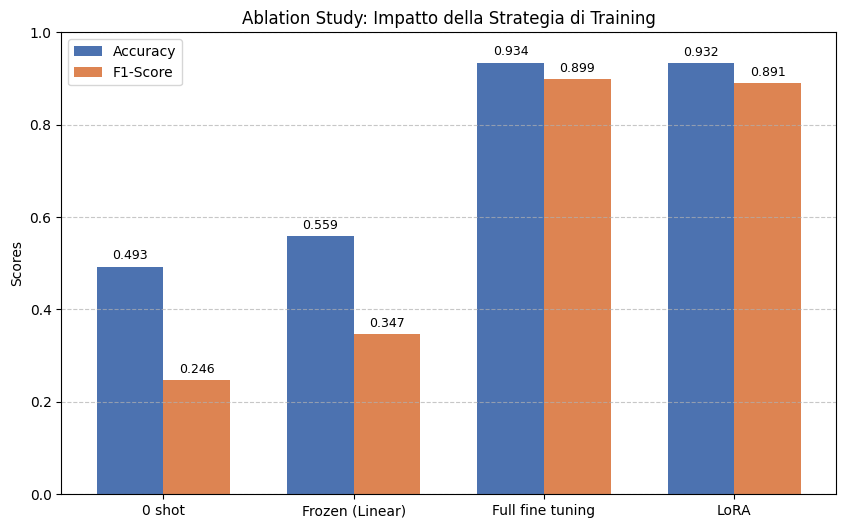
\includegraphics[width=0.85\textwidth]{img/ablation_chart.png}
    \caption{Confronto visivo delle Accuracy tra le strategie testate. Si nota il netto divario tra i metodi Frozen e LoRA.}
    \label{fig:ablation_chart}
\end{figure}

In conclusione, la tabella riassuntiva delle migliori configurazioni per categoria è la seguente:

\begin{table}[H]
    \centering
    \renewcommand{\arraystretch}{1.3}
    \begin{tabular}{|l|c|c|p{8cm}|}
        \hline
        \textbf{Strategia}        & \textbf{Accuracy} & \textbf{F1}      & \textbf{Conclusioni}                                                     \\
        \hline
        In-Context ($k=0$)        & 49.30\%           & 24.63\%          & Inadatto per task emotivi specifici.                                     \\
        \hline
        Transfer Learning         & 55.90\%           & 34.70\%          & Limitato dalle feature pre-addestrate.                                   \\
        \hline
        LoRA ($r=16$, all-linear) & 93.20\%           & 89.10\%          & Ottimo rapporto parametri/prestazioni.                                   \\
        \hline
        \textbf{Full Fine Tuning} & \textbf{93.40\%}  & \textbf{89.90\%} & \textbf{Best Model}. Aggiornamento completo dei pesi con $LR = 3e^{-5}$. \\
        \hline
    \end{tabular}
    \caption{Riepilogo finale Ablation Study}
    \label{tab:final_summary}
\end{table}

\subsubsection{Discussione dei Risultati}
I risultati ottenuti confermano che il Full Fine Tuning su un modello pre-addestrato su dominio specifico
costituisce un approccio estremamente efficace per task di classificazione emotiva.
Raggiungere un'accuratezza del 93.40\% aggiornando l'intero insieme di parametri ha permesso al modello
di adattarsi profondamente alle caratteristiche del linguaggio informale tipico dei social media.
L'elevato Macro F1-Score (89.90\%) conferma che il modello non è collassato sulle classi maggioritarie
(come \textit{Joy} o \textit{Sadness}), ma ha imparato a discriminare con efficacia anche le emozioni
meno frequenti nel dataset.

Tuttavia, l'analisi qualitativa degli errori, supportata dalla Matrice di Confusione (Figura \ref{fig:confusion_matrix}), ha rivelato che la maggior parte delle misclassificazioni residue non è casuale, ma si concentra su specifiche coppie di emozioni semanticamente vicine o contestualmente ambigue:

\begin{enumerate}
    \item \textbf{Love vs Joy:} Questa rappresenta la confusione più frequente, con il 10\% degli esempi di \textit{Love} classificati erroneamente come \textit{Joy}. È dovuta alla forte sovrapposizione semantica nei testi brevi tipici dei social network, dove parole di affetto, forte apprezzamento ed entusiasmo vengono usate in modo intercambiabile. Frasi che esprimono una profonda gioia spesso contengono termini legati all'amore (es. "I absolutely love this!"), rendendo il confine decisionale estremamente sfumato, a volte anche per un annotatore umano.

    \item \textbf{Fear vs Surprise:} Il 10\% degli esempi di \textit{Surprise} viene classificato erroneamente come \textit{Fear}, e il 4\% degli esempi di \textit{Fear} come \textit{Surprise}. Nei tweet, intrinsecamente brevi e spesso privi di contesto esteso, la reazione a un evento scioccante risulta difficile da disambiguare: senza abbastanza indizi testuali, il modello fatica a distinguere se la sorpresa sia di natura neutra/positiva oppure legata a una minaccia.
\end{enumerate}

Le classi meglio classificate sono \textit{Sadness} (98\%) e \textit{Joy} (96\%), probabilmente grazie alla loro maggiore frequenza nel dataset e alla ricchezza del loro vocabolario caratteristico. \textit{Surprise} risulta la classe più difficile (88\%), coerentemente con la sua natura semanticamente ibrida.

\begin{figure}[H]
    \centering
    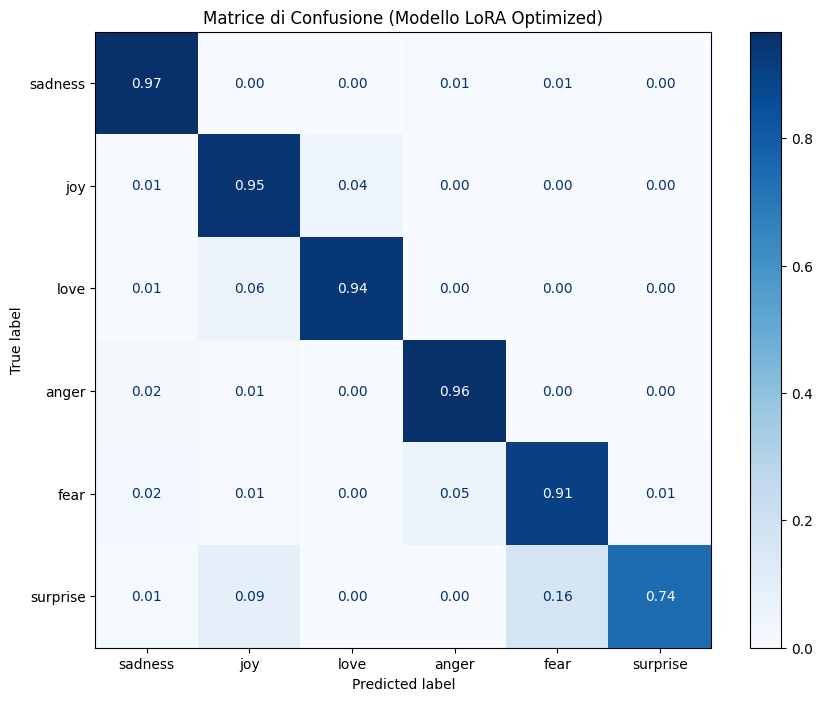
\includegraphics[width=0.75\textwidth]{img/confusion_matrix.png}
    \caption{Matrice di Confusione del modello Full Fine Tuning.}
    \label{fig:confusion_matrix}
\end{figure}
\subsubsection{Validità del Metodo}
Il metodo di Full Fine Tuning si è dimostrato la strategia più efficace, confermando che l'aggiornamento completo
dei pesi su un modello pre-addestrato su dominio specifico rappresenta la scelta ottimale quando le risorse
computazionali lo consentono. LoRA ha ottenuto risultati comparabili (93.20\% di Accuracy) con un numero
significativamente inferiore di parametri addestrabili, rappresentando un'alternativa valida in contesti
con vincoli di memoria o tempo. Al contrario, lo studio di ablation su \textbf{In-Context Learning}
ha evidenziato un limite strutturale critico: l'architettura BERTweet, progettata con una finestra di contesto
ridotta (128 token), \textbf{non è idonea} a strategie Few-Shot ($k>3$). Gli esempi dimostrativi tendono a
saturare la memoria e troncare il prompt, peggiorando le performance invece di migliorarle, rendendo il
fine-tuning una scelta obbligata per questo tipo di architetture.
\subsection{distilbert-base-uncased}
Il modello scelto è \textbf{DistilBERT-base-uncased}, un modello di tipo encoder derivato da BERT, progettato per essere più leggero e veloce mantenendo buone prestazioni.

Presenta le seguenti proprietà:

\begin{itemize}
    \item Parametri: 66M
    \item Lingua: English
    \item Tensor type: F32
    \item Versione uncased
    \item Architettura Transformer encoder distillata
\end{itemize}

Il modello eredita il pre-training basato su:

\begin{itemize}
    \item \textbf{Masked Language Modelling (MLM)}: viene mascherato casualmente il 15\% delle parole nell’input; il modello deve prevedere i token mascherati a partire dal contesto circostante.
\end{itemize}

A differenza di BERT, DistilBERT non utilizza il task Next Sentence Prediction (NSP) durante il pre-training, rendendo il processo più efficiente e riducendo la complessità del modello.


\subsubsection{Selezione dei parametri di training}

Una fase cruciale in questo tipo di scenari è rappresentata da come viene svolto l’addestramento del modello. Questo è in larga parte delineato dalla selezione dei parametri di addestramento. Nel nostro caso ci siamo soffermati sui seguenti:

\begin{itemize}
    \item Number of Epochs: quante volte l’intero training set viene processato
    \item Learning rate: la dimensione dei passi di addestramento
    \item Weight decay: evita che i parametri crescano troppo
    \item Train Batch Size: dimensione di batch di training per device
\end{itemize}

Gli altri valori configurativi sono stati mantenuti alle impostazioni predefinite.

\subsubsection{Parametri per Classification Head Alignment}

\begin{table}[H]
    \centering
    \begin{tabular}{lc}
        \toprule
        Learning Rate    & 3e-3 \\
        Weight Decay     & 0.01 \\
        Number of Epochs & 15   \\
        Train Batch Size & 16   \\
        \bottomrule
    \end{tabular}
    \caption{Parametri per classification head alignment}
\end{table}

Per l'allineamento del classification head di Distilbert è stato utilizzato un learning rate pari a $3 \times 10^{-3}$, valore più elevato rispetto a quello tipicamente impiegato nel fine-tuning completo dei transformer. Questa scelta è coerente con lo scenario di light fine-tuning, in cui il backbone pre-addestrato rimane congelato e viene aggiornato il livello di classificazione, inizializzato casualmente. Un learning rate più alto consente quindi al classificatore di adattarsi rapidamente alle rappresentazioni già strutturate fornite dal modello pre-addestrato, favorendo una convergenza più veloce senza compromettere la stabilità del training.

È stato inoltre impostato un weight decay pari a 0.01, con funzione di regolarizzazione L2 sui pesi del classification head. Questa scelta contribuisce a limitare la crescita eccessiva dei parametri, riducendo il rischio di overfitting e migliorando la capacità di generalizzazione.

Il batch size di 16 rappresenta un compromesso tra stabilità dell’ottimizzazione e vincoli computazionali, introducendo una moderata variabilità stocastica nei gradienti che può favorire la generalizzazione.

Il numero di epoche è stato fissato a 15: durante le prove è stato osservato che proseguendo oltre, anche per molte epoche aggiuntive, la validation loss rimaneva sostanzialmente stabile, con variazioni minime. Per questo motivo si è scelto di interrompere il training a 15 epoche, in quanto il modello aveva già raggiunto una fase di convergenza e ulteriori iterazioni non portavano miglioramenti significativi.

\begin{figure}[H]
    \centering
    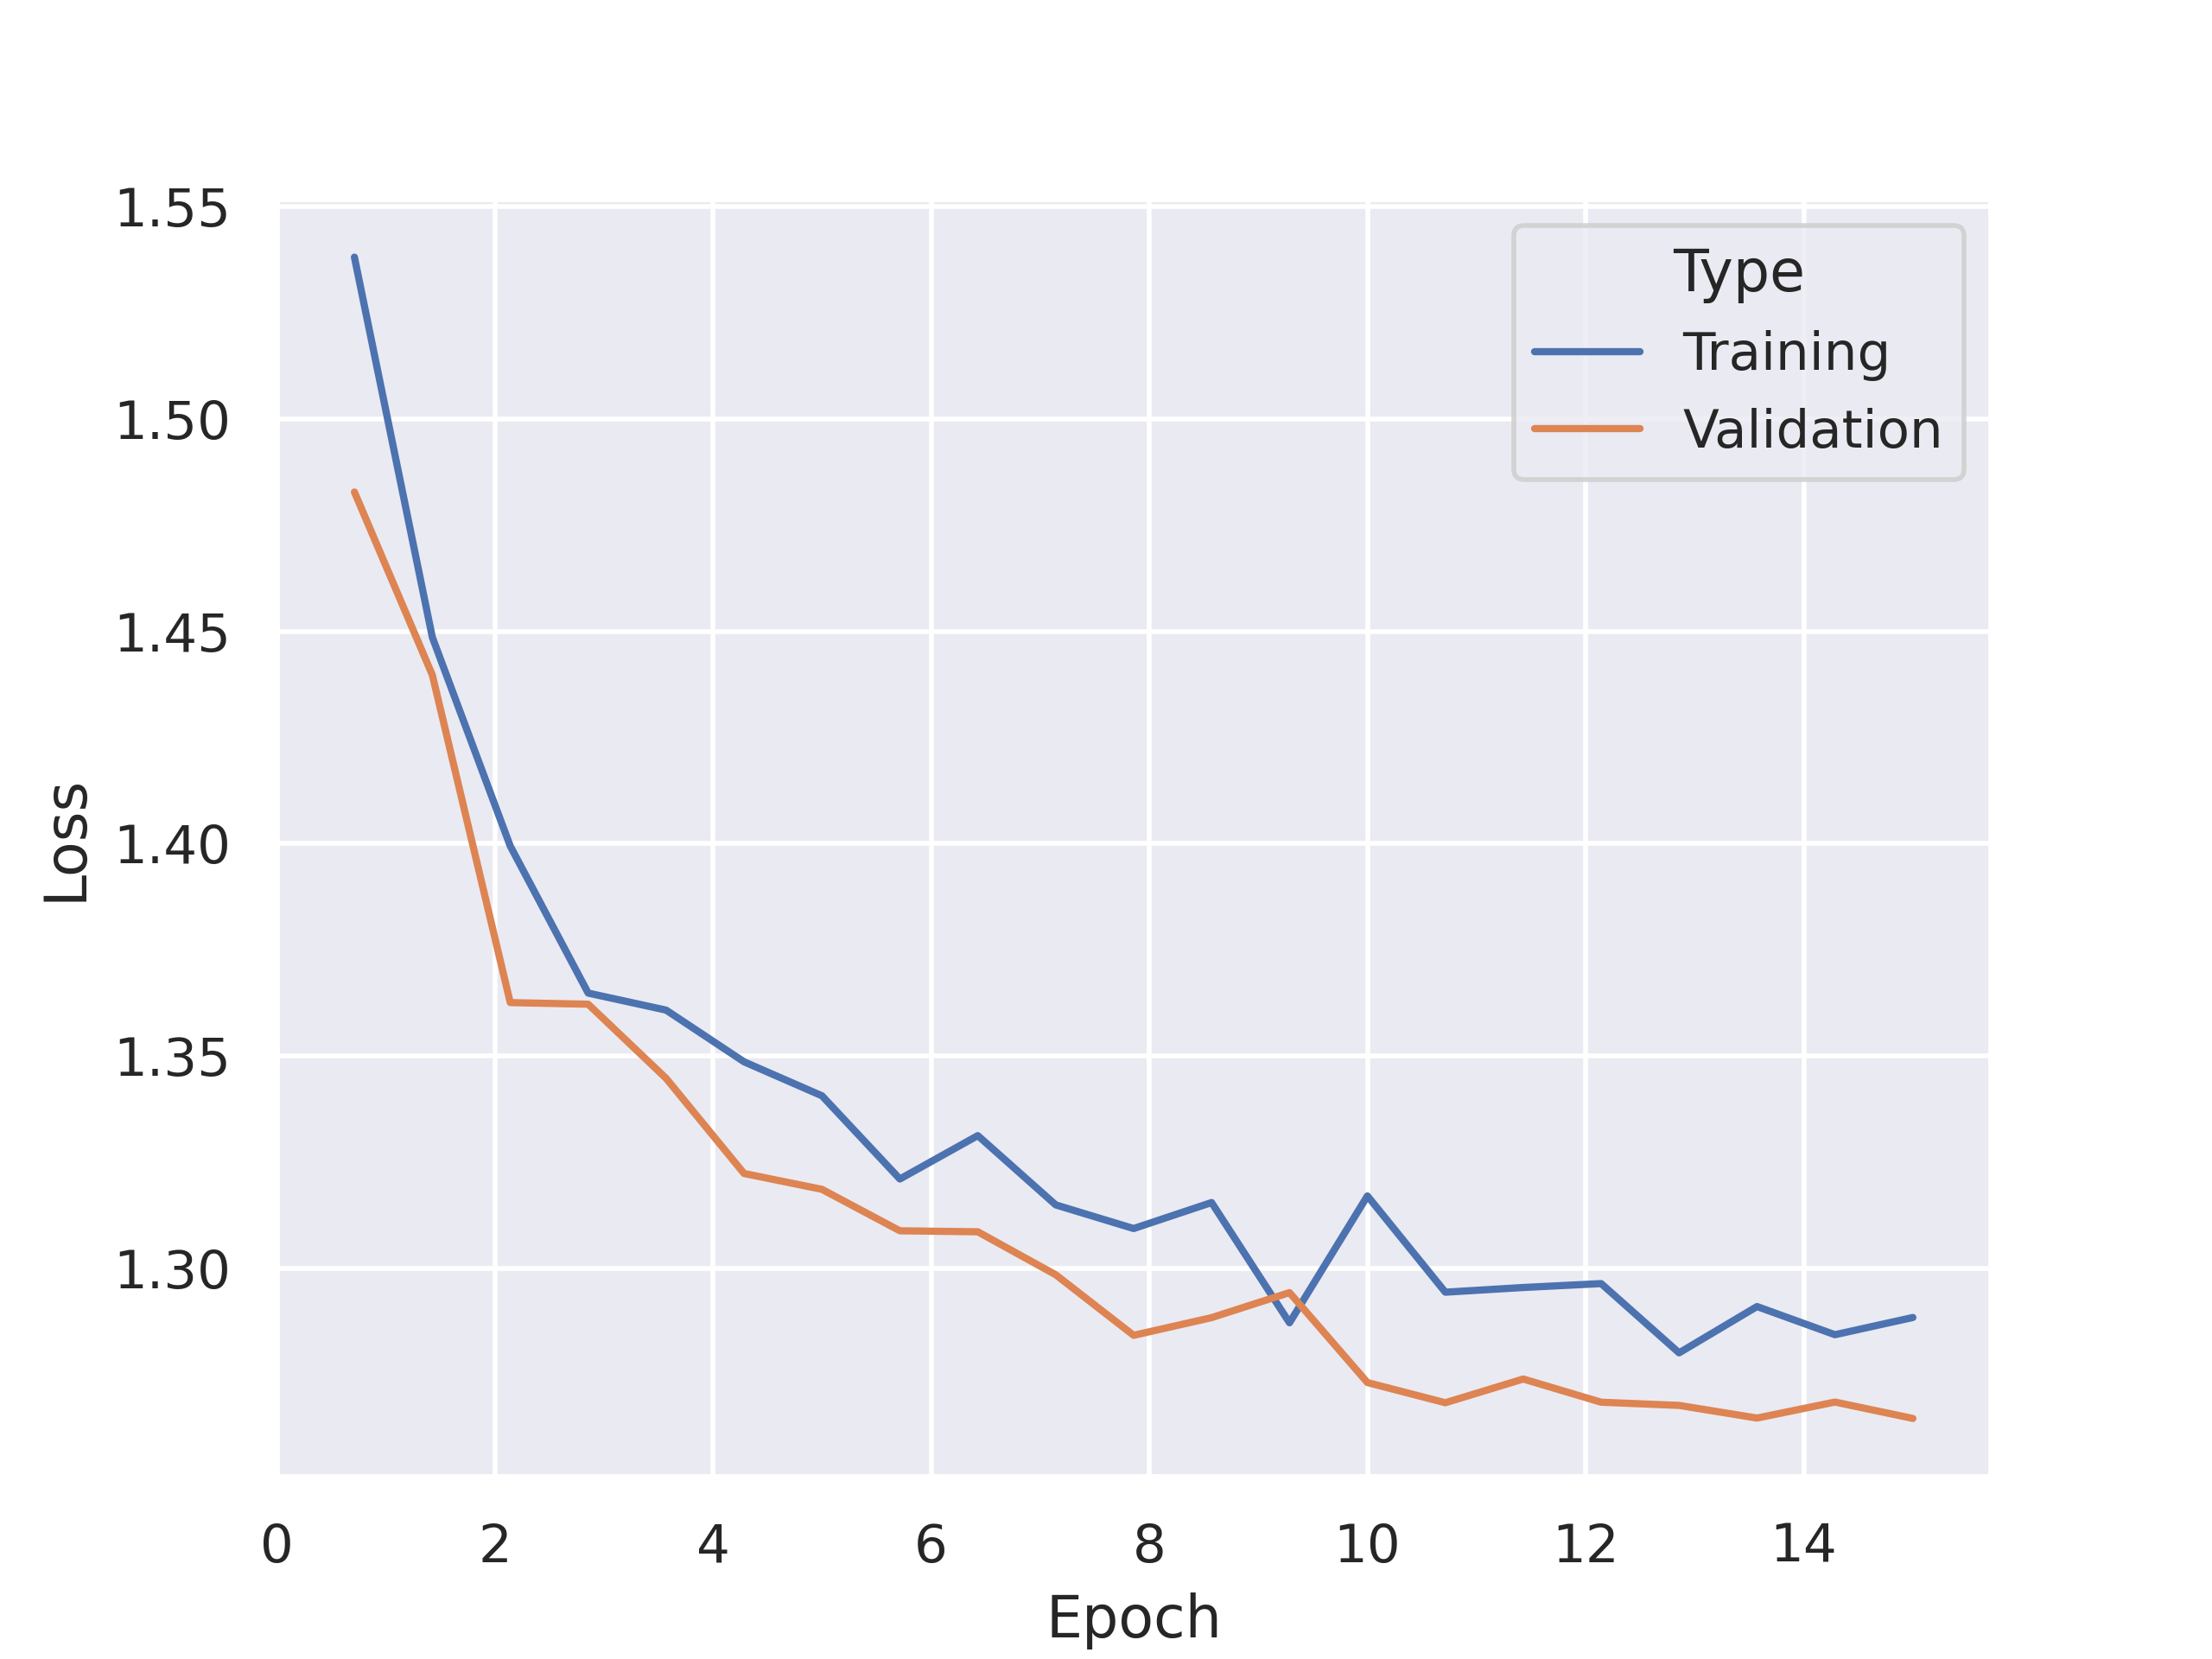
\includegraphics[width=0.8\textwidth]{img/distilbert/Light_FT_loss.png}
    \caption{Training e Validation Loss - Classification Head Alignment}
\end{figure}

Il grafico della loss mostra un andamento decrescente sia per il training che per la validation, con una riduzione più marcata nelle prime epoche e un successivo rallentamento del miglioramento. Nella fase iniziale il classification head si adatta rapidamente alle rappresentazioni fornite dal backbone di DistilBERT, determinando un calo evidente della loss. Successivamente la diminuzione diventa più graduale, segno che il modello entra in una fase di raffinamento dei pesi.

Le curve di training e validation rimangono molto vicine lungo tutto il processo, senza divergenze significative. Questo comportamento indica assenza di overfitting marcato e una buona capacità di generalizzazione del classificatore. Nelle ultime epoche la validation loss tende a stabilizzarsi, mostrando variazioni molto contenute: tale plateau ha motivato la scelta di interrompere il training a 15 epoche, poiché ulteriori iterazioni non avrebbero apportato miglioramenti sostanziali.

\begin{figure}[H]
    \centering
    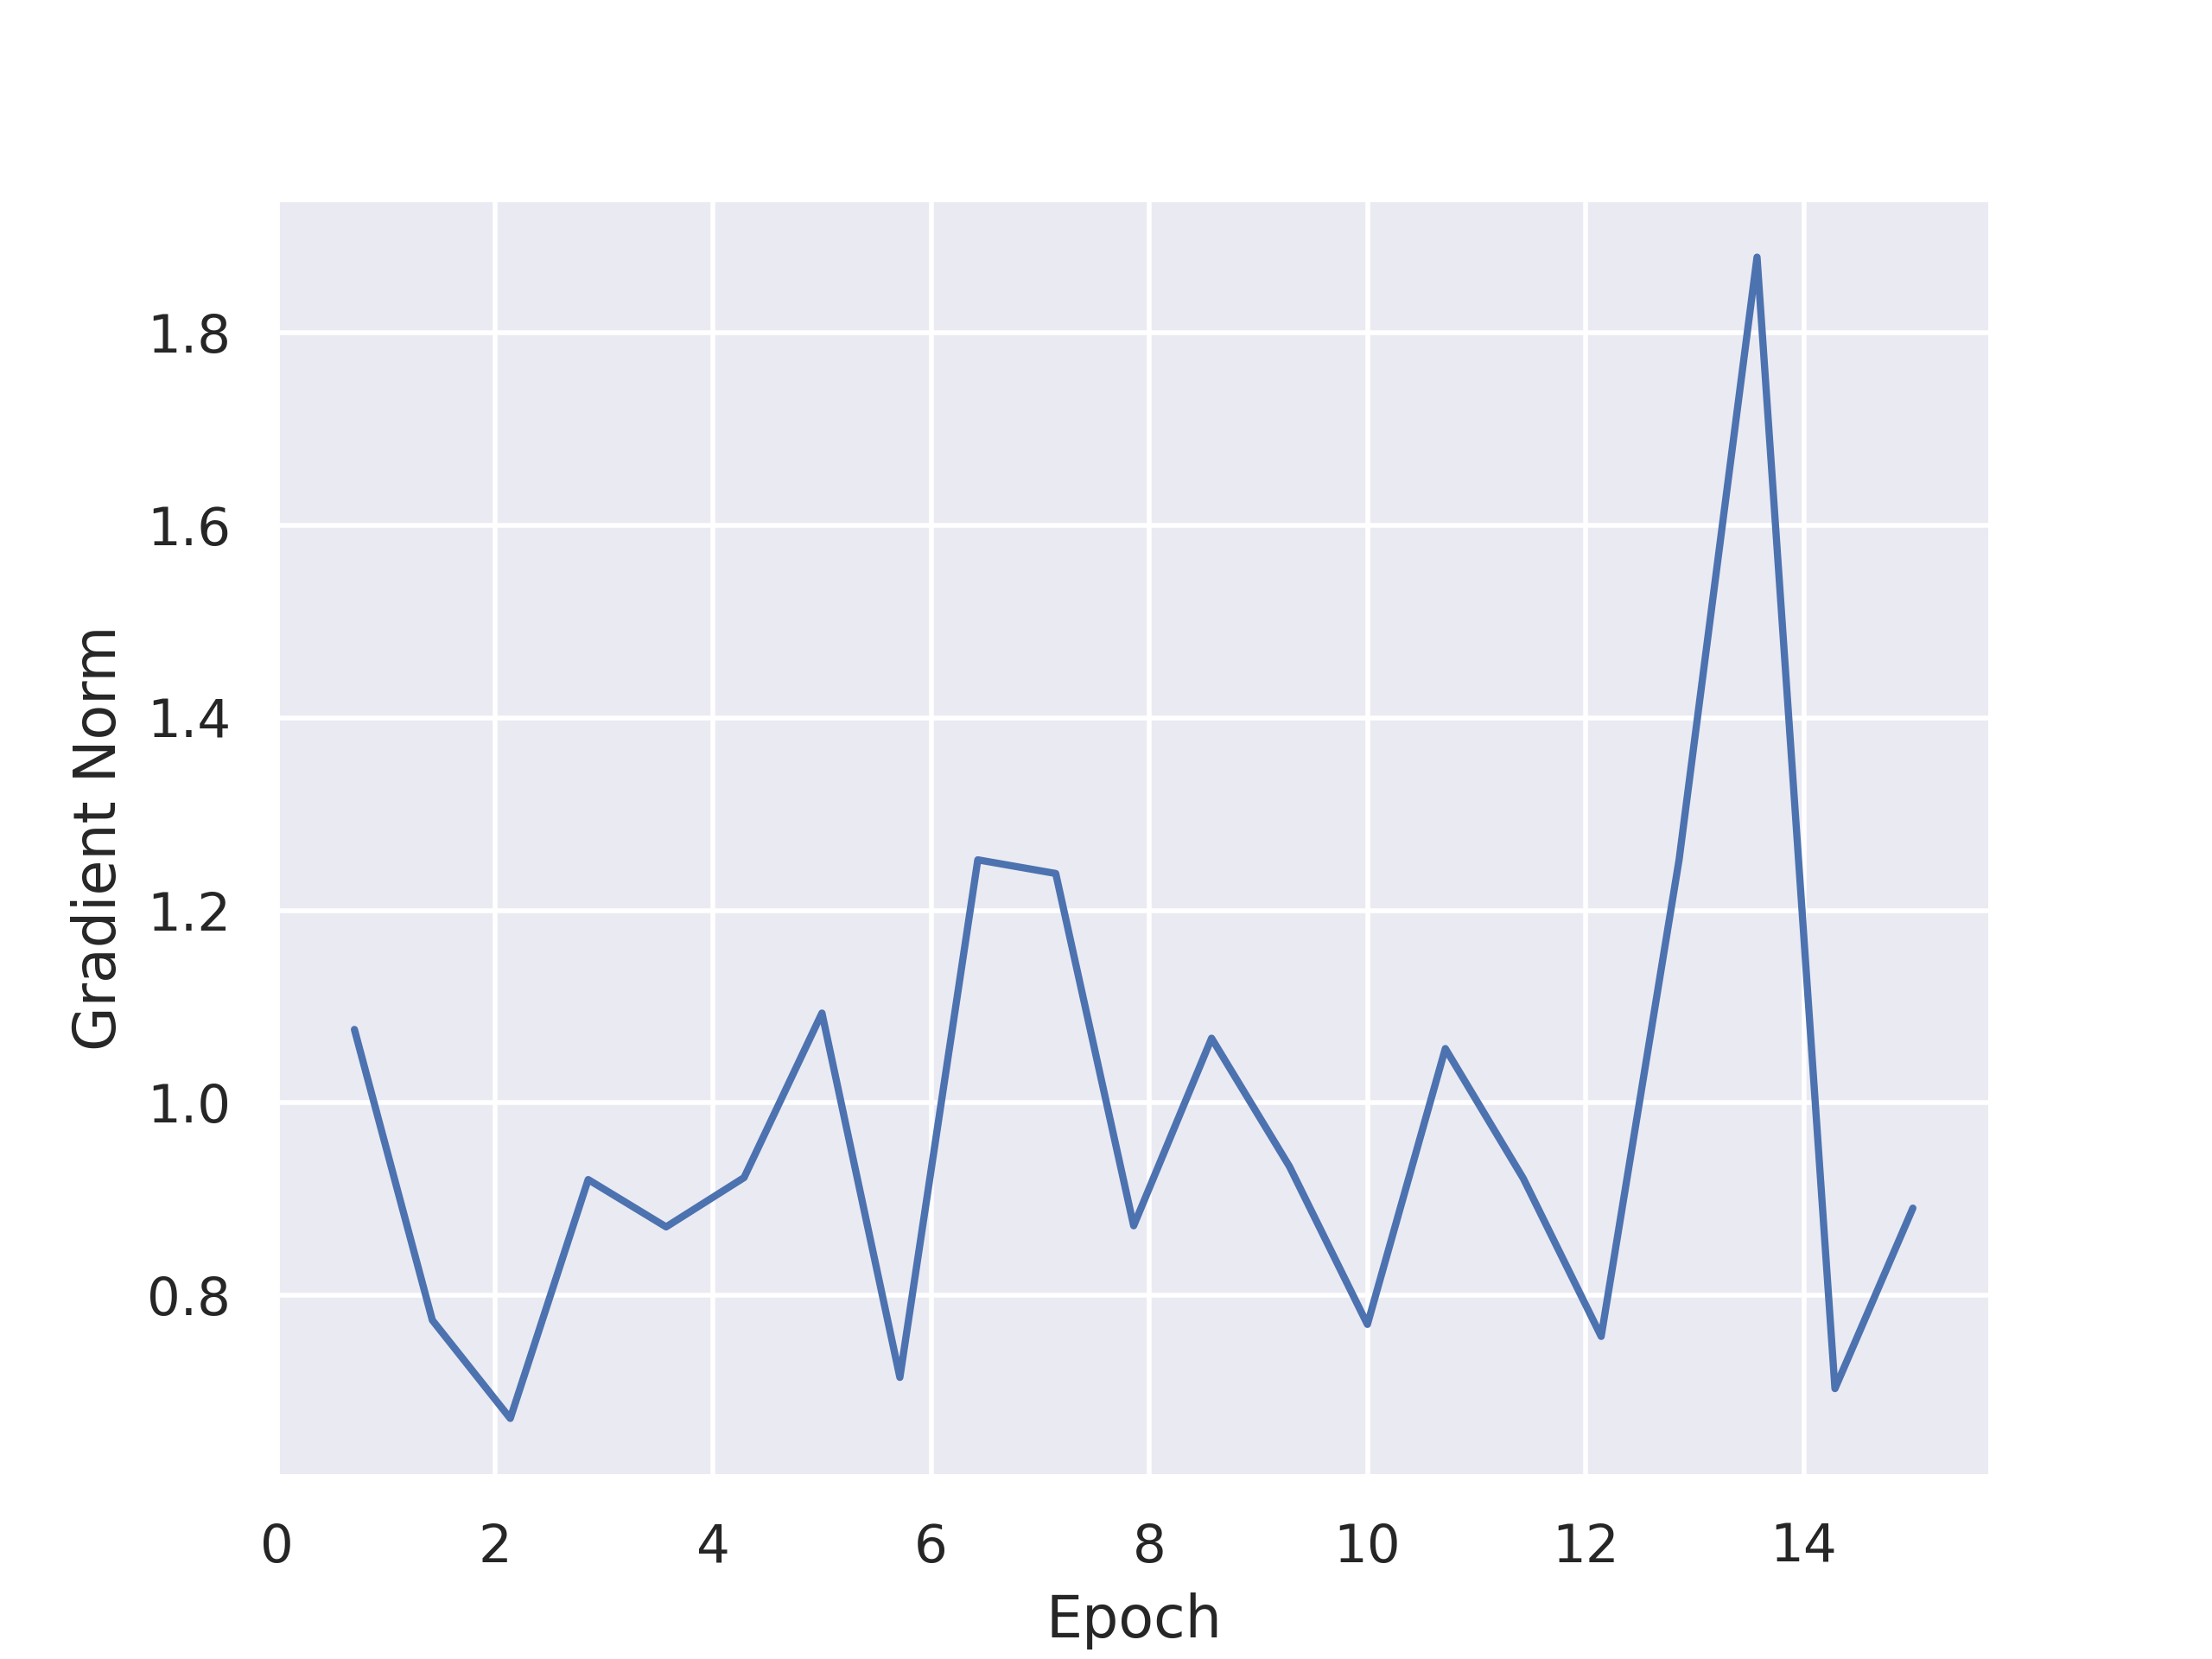
\includegraphics[width=0.8\textwidth]{img/distilbert/Light_FT_gradnorm.png}
    \caption{Gradient Norm - Classification Head Alignment}
\end{figure}

Il grafico della norma del gradiente evidenzia valori generalmente compresi in un intervallo stabile, con oscillazioni moderate tra un’epoca e l’altra. Questo comportamento è coerente con l’utilizzo di un batch size pari a 16, che introduce una componente stocastica negli aggiornamenti, e con il fatto che si stia ottimizzando principalmente il classification head. Le variazioni osservate riflettono la normale dinamica dell’ottimizzazione in un contesto non deterministico.

Si nota un picco isolato nelle ultime epoche, ma non si osservano fenomeni di esplosione persistente del gradiente né instabilità prolungate. Il valore rientra rapidamente nei range precedenti, indicando che il processo di training rimane numericamente stabile. Nel complesso, l’andamento della norma del gradiente conferma che l’ottimizzazione è avvenuta in modo controllato e coerente con un corretto allineamento del classification head alle rappresentazioni interne di DistilBERT.


\subsubsection{Parametri Fine-tuning Completo}

\begin{table}[H]
    \centering
    \begin{tabular}{lc}
        \toprule
        Learning Rate & 3e-5 \\
        Weight Decay  & 0.01 \\
        Max Epochs    & 14   \\
        Batch Size    & 16   \\
        \bottomrule
    \end{tabular}
    \caption{Parametri per fine-tuning completo}
\end{table}

Per il fine-tuning completo del modello DistilBERT, sono stati adottati parametri più conservativi rispetto alla fase di addestramento della sola classification head, in quanto in questa fase vengono aggiornati tutti i pesi del modello pre-addestrato.

Il learning rate pari a $3 \times 10^{-5}$ è stato scelto in linea con le pratiche consolidate per il fine-tuning dei modelli Transformer pre-addestrati. In letteratura e nella documentazione ufficiale dei modelli basati su BERT e DistilBERT, il range tipicamente raccomandato per il learning rate è compreso tra 1e-5 e 5e-5. L’utilizzo di un valore contenuto consente di preservare le conoscenze linguistiche acquisite durante il pre-training, evitando aggiornamenti troppo aggressivi che potrebbero degradare le rappresentazioni interne del modello.

Il weight decay pari a 0.01 è stato mantenuto per introdurre regolarizzazione L2 e migliorare la capacità di generalizzazione, limitando fenomeni di overfitting durante l’aggiornamento di tutti i parametri del modello.

Il numero massimo di 14 epoche è stato inizialmente impostato considerando che, nel fine-tuning di modelli pre-addestrati, sono generalmente sufficienti poche epoche per adattare efficacemente il modello al task specifico, mentre un numero eccessivo potrebbe aumentare il rischio di overfitting. Tuttavia, dall’analisi dell’andamento della loss si è osservato che i valori migliori di validation loss si raggiungono già intorno all’epoca 1.75. Dopo questo punto, la training loss continua a diminuire rapidamente, mentre la validation loss inizia progressivamente ad aumentare, evidenziando un chiaro fenomeno di overfitting. Per questo motivo, pur avendo impostato 14 epoche come limite massimo, si è scelto di interrompere il training anticipatamente all’epoca 1.75, corrispondente alla configurazione con le migliori prestazioni in termini di generalizzazione nel fine-tuning completo.

Infine, la batch size pari a 16 rappresenta un compromesso tra stabilità dell’aggiornamento del gradiente e limiti di memoria GPU, garantendo un training efficiente e stabile.

\begin{figure}[H]
    \centering
    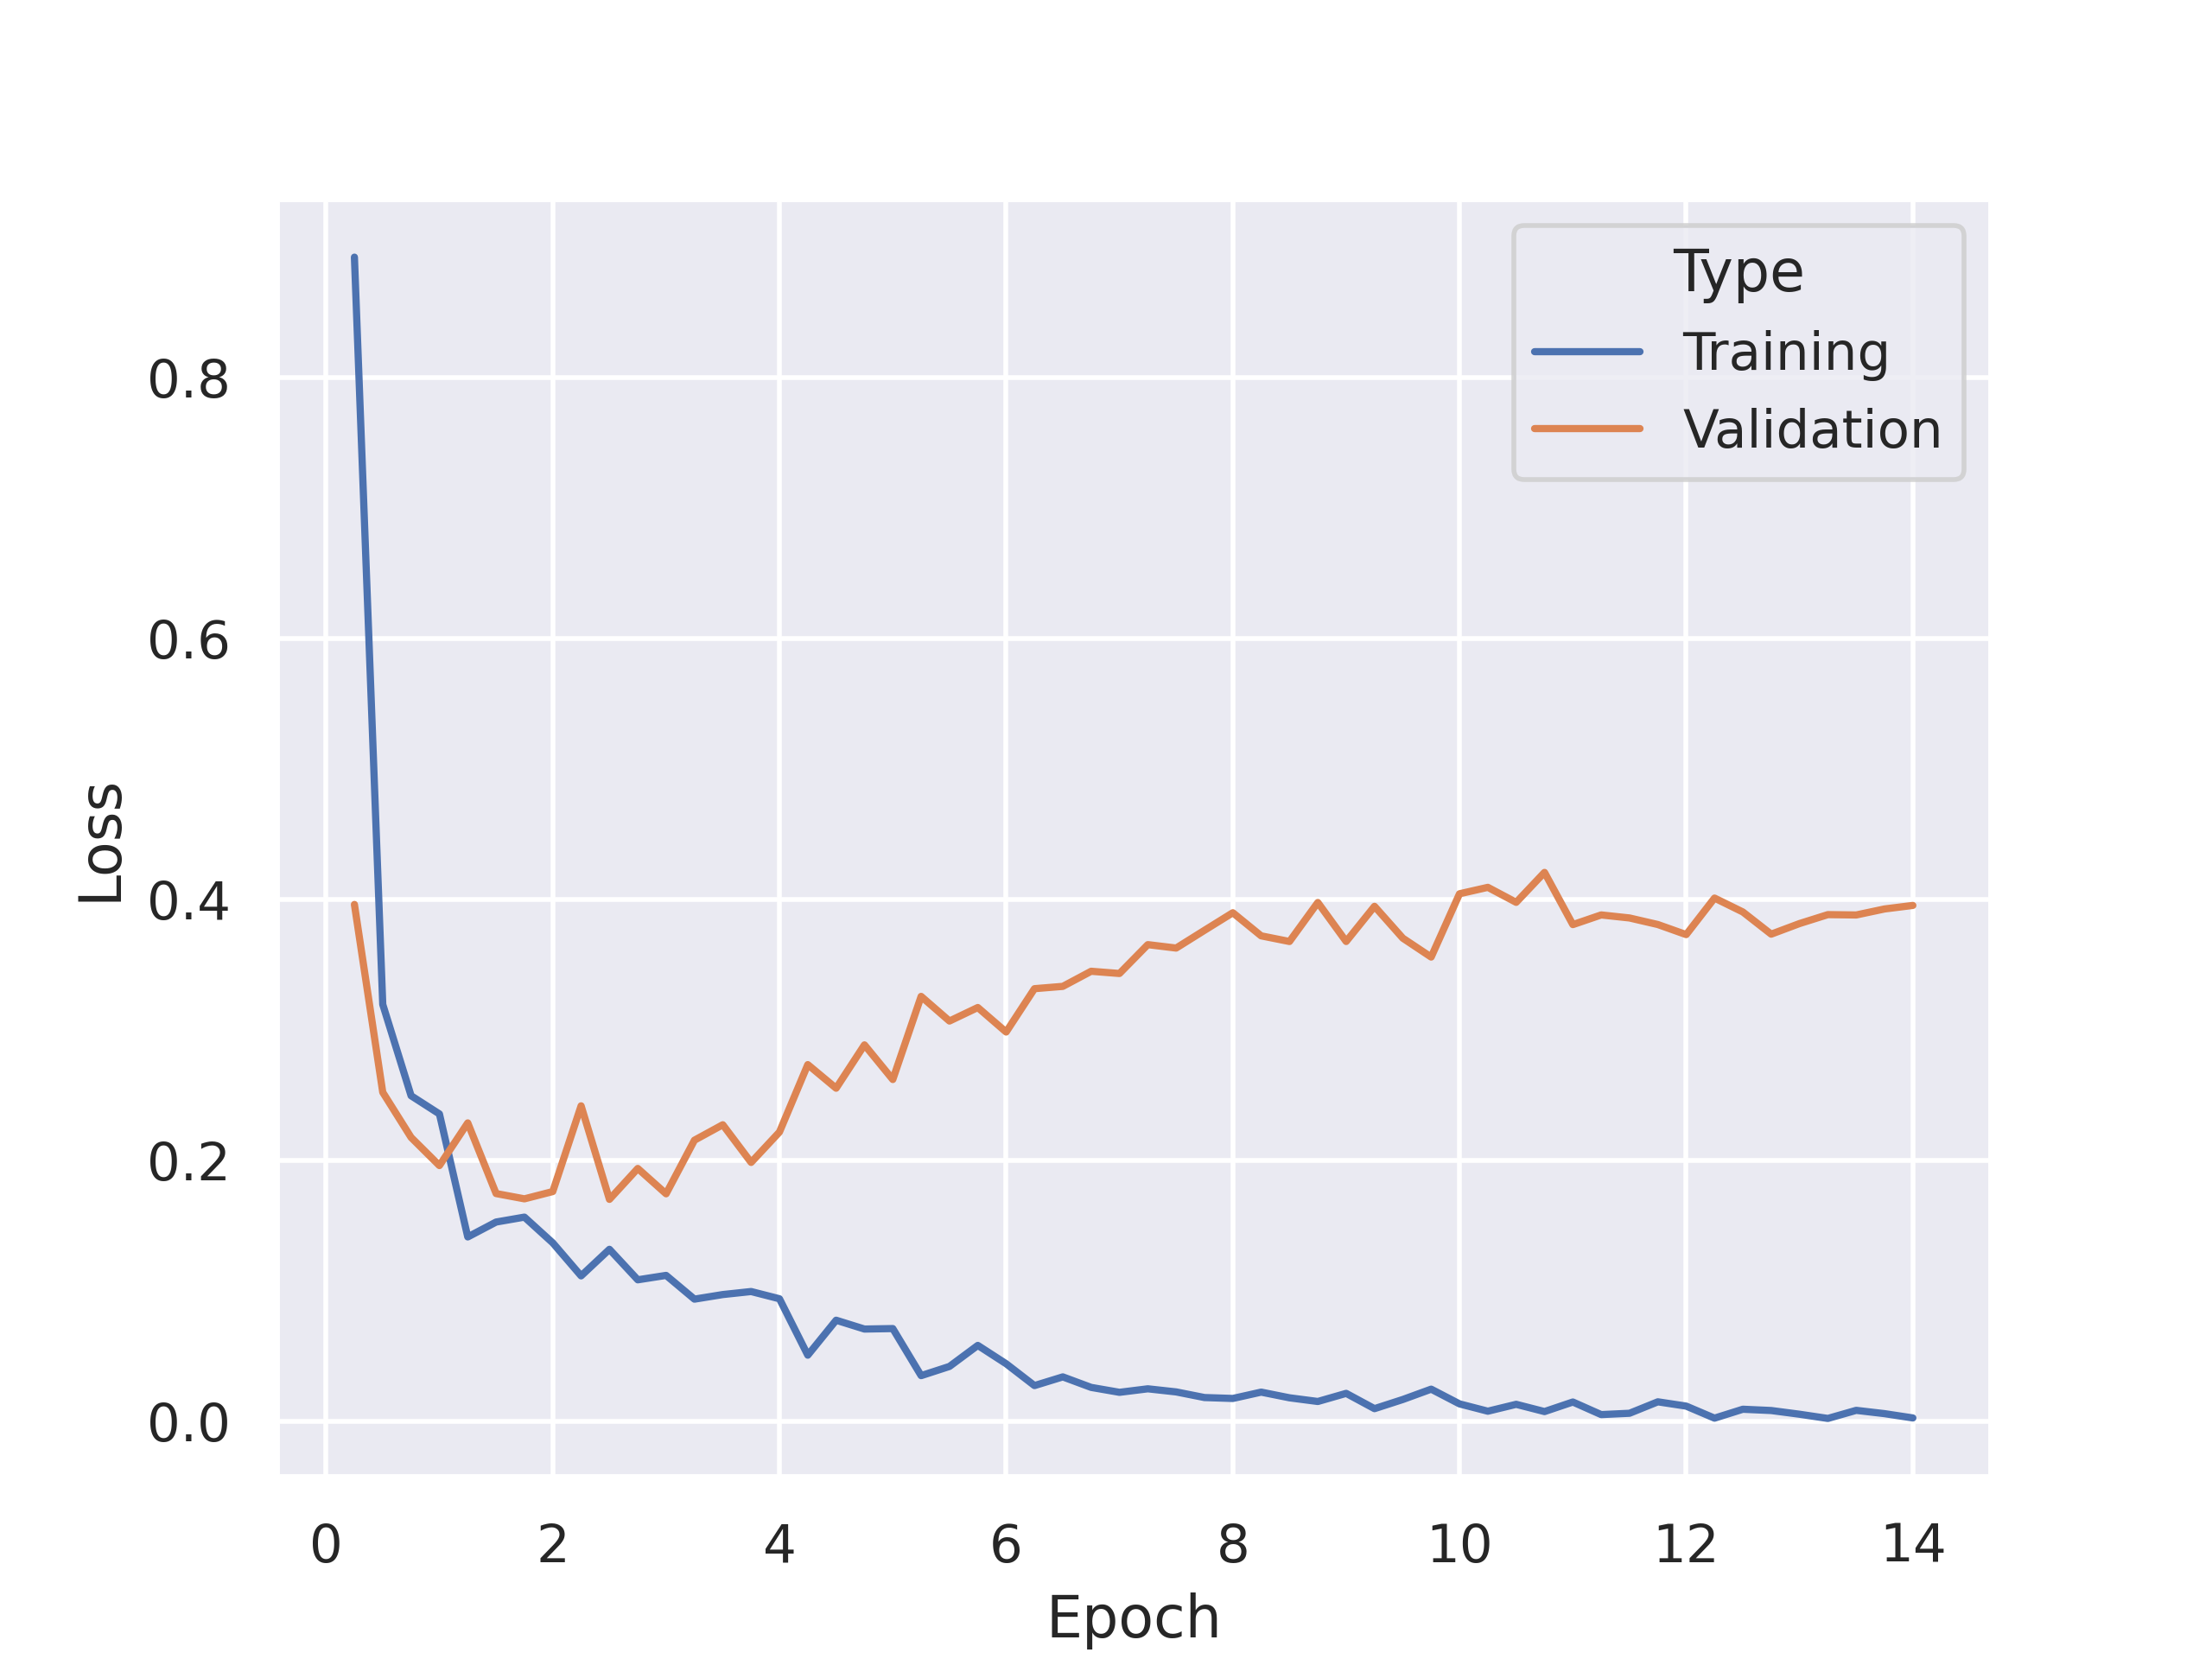
\includegraphics[width=0.8\textwidth]{img/distilbert/Complete_FT_loss.png}
    \caption{Training e Validation Loss - Fine-tuning Completo}
\end{figure}

Nel grafico viene riportato l’andamento della training loss e della validation loss nel corso delle epoche.

Si osserva che:

\begin{enumerate}
    \item La training loss decresce rapidamente fin dalle prime epoche, passando da un valore iniziale elevato (circa 0.9) a valori prossimi allo zero nelle epoche successive.

    \item La validation loss, invece, diminuisce solo nelle primissime fasi del training, raggiungendo il valore minimo intorno all’epoca 1.75.
\end{enumerate}

Dopo l’epoca 1.75, mentre la training loss continua a diminuire, la validation loss inizia progressivamente ad aumentare. Questo andamento evidenzia chiaramente un fenomeno di \textbf{overfitting}: il modello continua a migliorare sulle istanze di training, ma peggiora sulle istanze di validazione, perdendo capacità di generalizzazione.

L’analisi del grafico conferma quindi la scelta metodologica di applicare \textit{early stopping} all’epoca 1.75, nonostante il limite massimo fosse stato impostato a 14 epoche. Il punto di minimo della validation loss rappresenta infatti la configurazione con il miglior compromesso tra apprendimento del task e mantenimento della capacità di generalizzazione.

\begin{figure}[H]
    \centering
    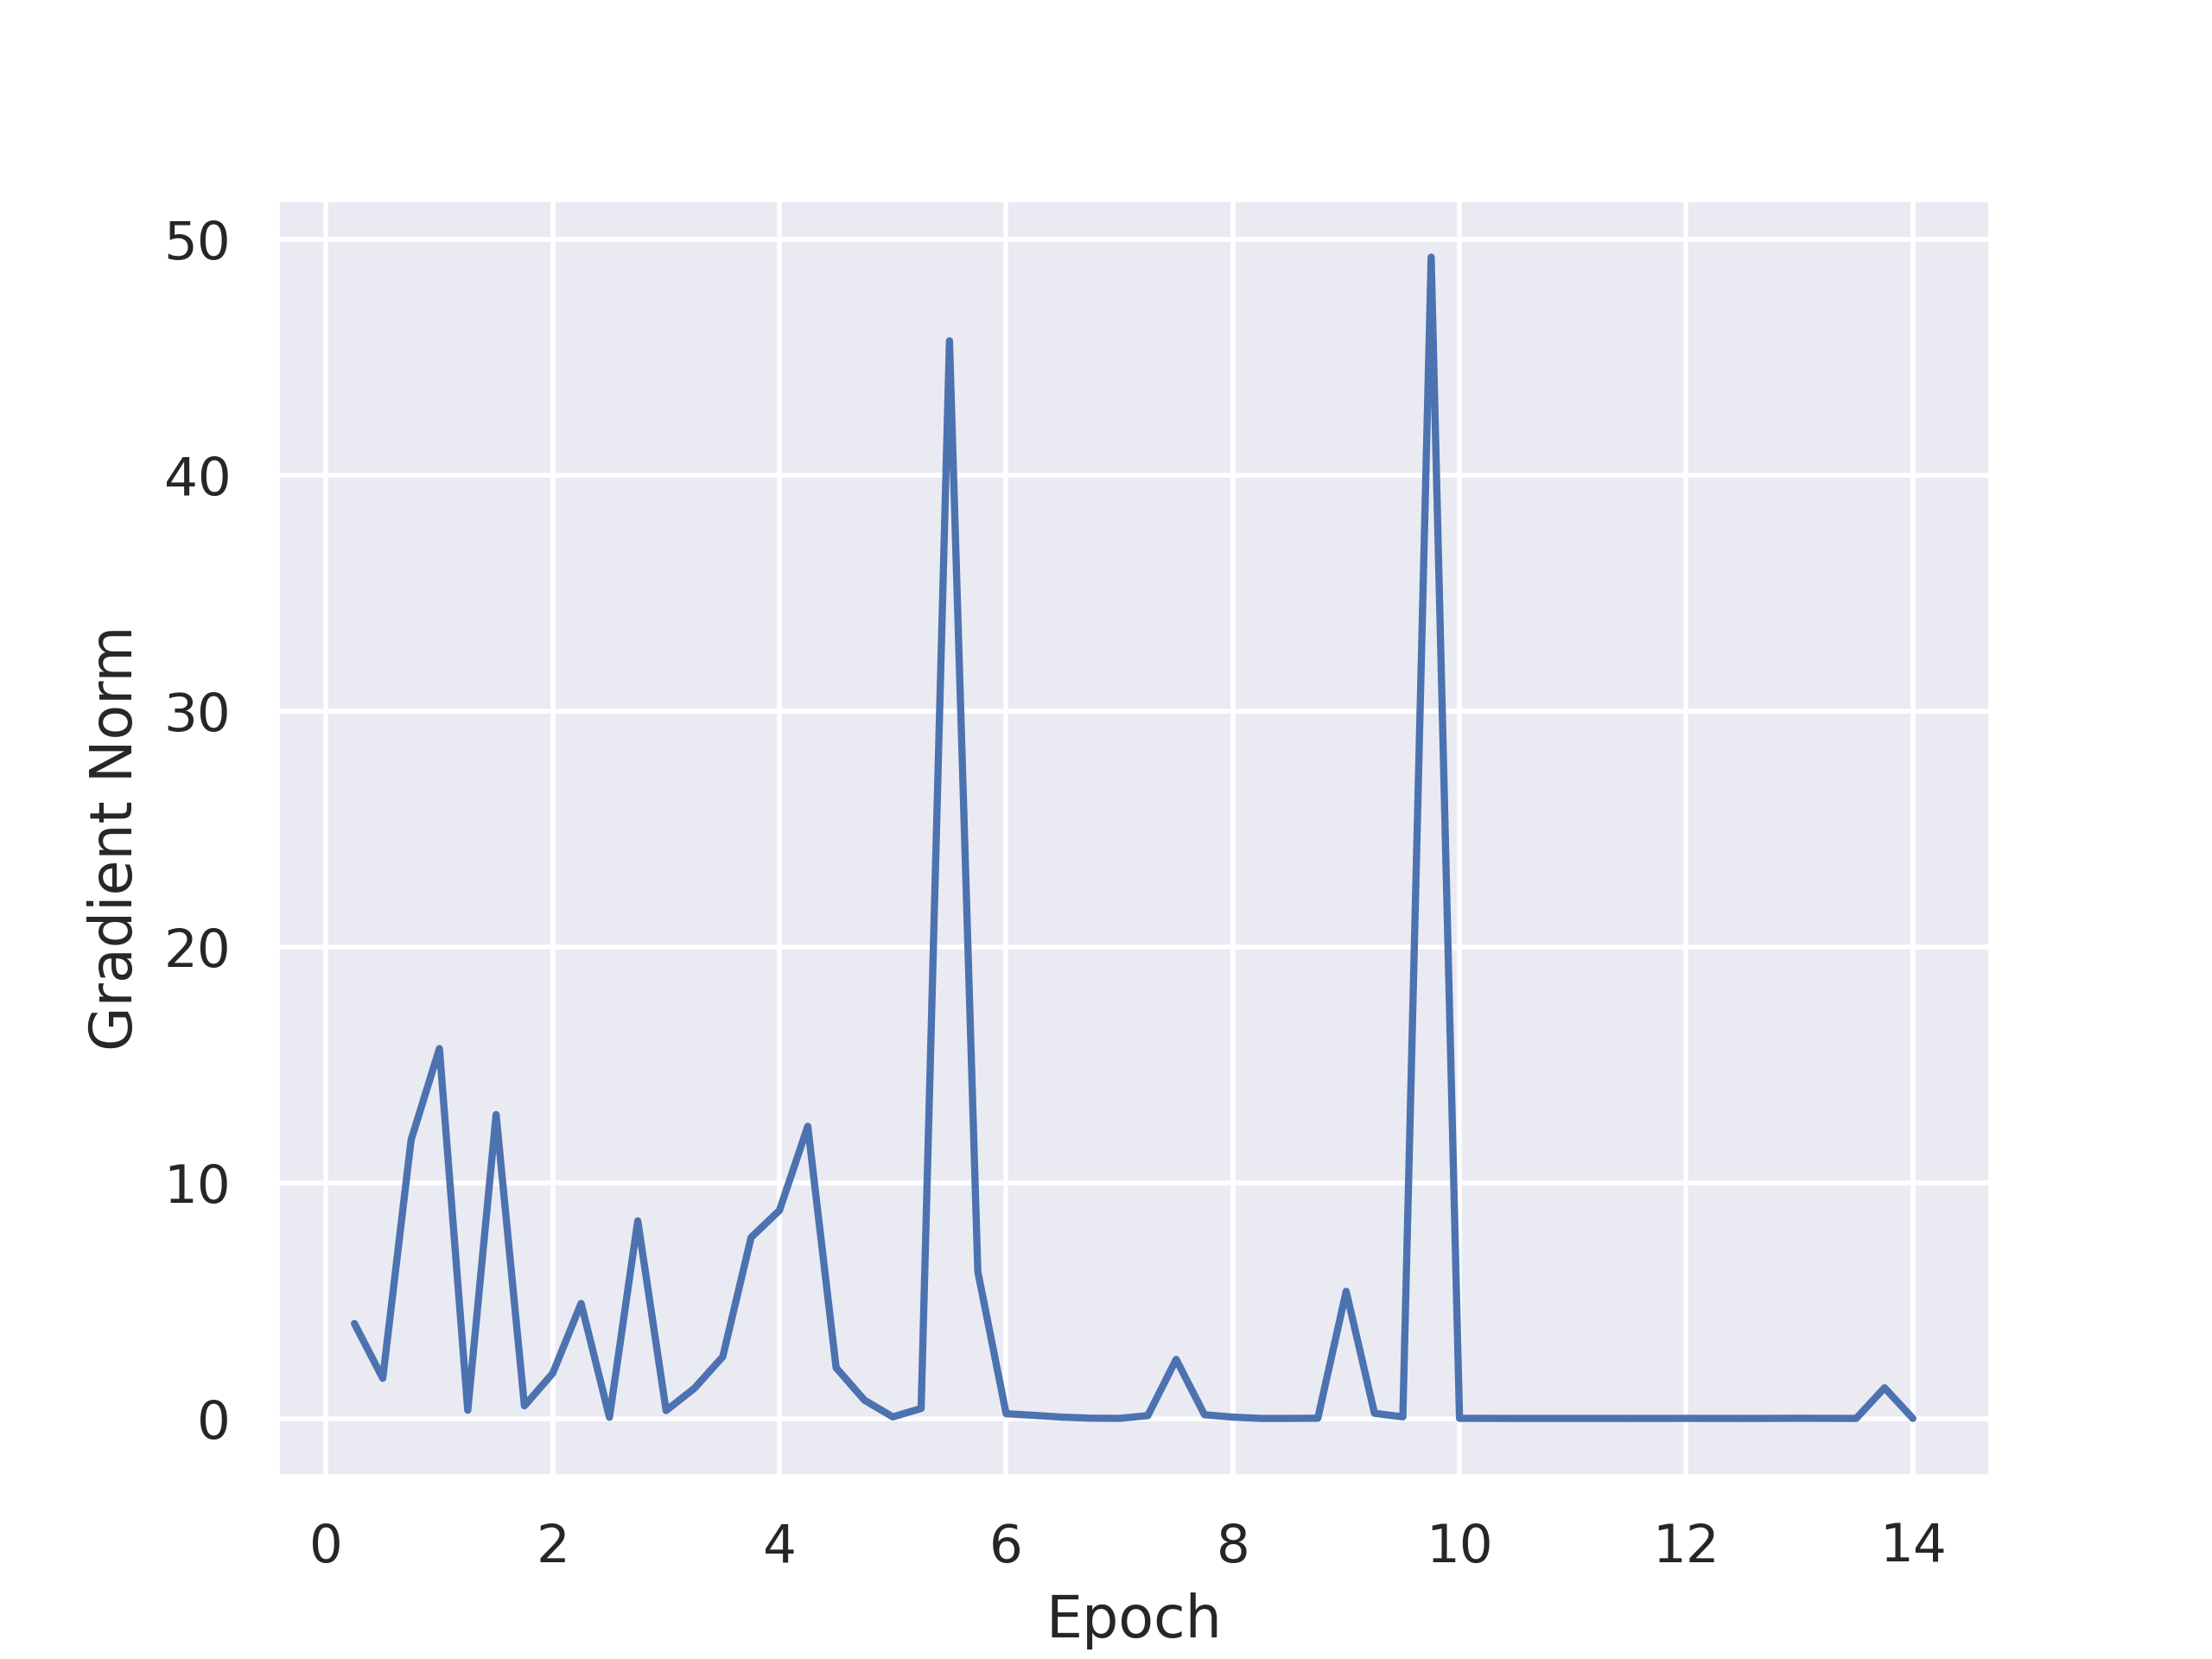
\includegraphics[width=0.8\textwidth]{img/distilbert/Complete_FT_gradnorm.png}
    \caption{Gradient Norm - Fine-tuning Completo}
\end{figure}

L’andamento della Gradient Norm mostra valori inizialmente più elevati e variabili nelle prime epoche, segno che il modello sta effettuando aggiornamenti significativi per adattarsi al nuovo task.

Intorno all’epoca 1.75 il modello ha già compiuto la parte più rilevante dell’apprendimento. Successivamente, la norma del gradiente tende a ridursi e stabilizzarsi su valori molto bassi, indicando una progressiva convergenza sul training set.

Poiché dopo l’epoca 1.75 la validation loss inizia ad aumentare, la diminuzione della gradient norm non corrisponde più a un miglioramento della generalizzazione ma a un adattamento eccessivo ai dati di training.

Pertanto, l’andamento della gradient norm risulta coerente con la scelta di applicare l’early stopping all’epoca 1.75, punto in cui il modello raggiunge il miglior compromesso tra apprendimento e capacità di generalizzazione.


\subsubsection{Risultati}

Di seguito vengono presentate le prestazioni ottenute dai modelli con i risultati migliori, sia nella versione light fine-tuned sia in quella fully fine-tuned.

\subsubsection*{Performance inContext Learning}

In questa sezione viene analizzata la capacità del modello, opportunamente allineato al task, di ottenere buone prestazioni mediante l’utilizzo della tecnica di in-context learning applicata al test set.

La valutazione è stata condotta considerando tre differenti livelli di fornitura di esempi:

\begin{enumerate}
    \item \textbf{One-shot}: il prompt contiene un unico esempio input-output che dimostra l'applicazione del task.

    \item \textbf{Three-shot}: il prompt contiene tre esempi input-output che dimostrano l'applicazione del task.

    \item \textbf{Five-shot}: il prompt contiene cinque esempi input-output che dimostrano l'applicazione del task.
\end{enumerate}

Per ciascuna configurazione di in-context learning considerata vengono riportati i principali risultati ottenuti dal modello. In particolare, per ogni configurazione vengono presentati l’accuracy complessiva e le metriche di precision, recall e F1-score calcolate per ciascuna classe. Queste ultime sono mostrate sia in forma tabellare sia tramite rappresentazione grafica al fine di facilitarne l’interpretazione e il confronto tra le diverse classi.

Inoltre, per ogni configurazione viene riportata la relativa confusion matrix, che consente di analizzare più nel dettaglio la distribuzione delle predizioni del modello. In tale matrice, le righe rappresentano le classi reali, mentre le colonne indicano le classi predette dal modello. I valori presenti sulla diagonale principale corrispondono alle classificazioni corrette, mentre i valori al di fuori della diagonale evidenziano gli errori di classificazione e permettono di individuare eventuali confusioni tra specifiche classi.

\subsubsection*{Performance One-Shot}

\begin{table}[H]
    \centering
    \begin{tabular}{cc}
        \toprule
        Metric & Value \\
        \midrule
        Accuracy & 0.4805 \\
        \bottomrule
    \end{tabular}
    \caption{Accuracy del modello in configurazione One-Shot}
\end{table}

\vspace{0.5cm}

\begin{table}[H]
    \centering
    \begin{tabular}{cccc}
        \toprule
        Class & Precision & Recall & F1 \\
        \midrule
        Sadness & 0.4575 & 0.5835 & 0.5129 \\
        Joy & 0.5577 & 0.7367 & 0.6348 \\
        Love & 0.0000 & 0.0000 & 0.0000 \\
        Anger & 0.0000 & 0.0000 & 0.0000 \\
        Fear & 0.3235 & 0.4911 & 0.3901 \\
        Surprise & 0.0000 & 0.0000 & 0.0000 \\
        \bottomrule
    \end{tabular}
    \caption{Metriche di precision, recall e F1 per classe in configurazione One-Shot}
\end{table}

\vspace{0.5cm}

\begin{figure}[H]
    \centering
    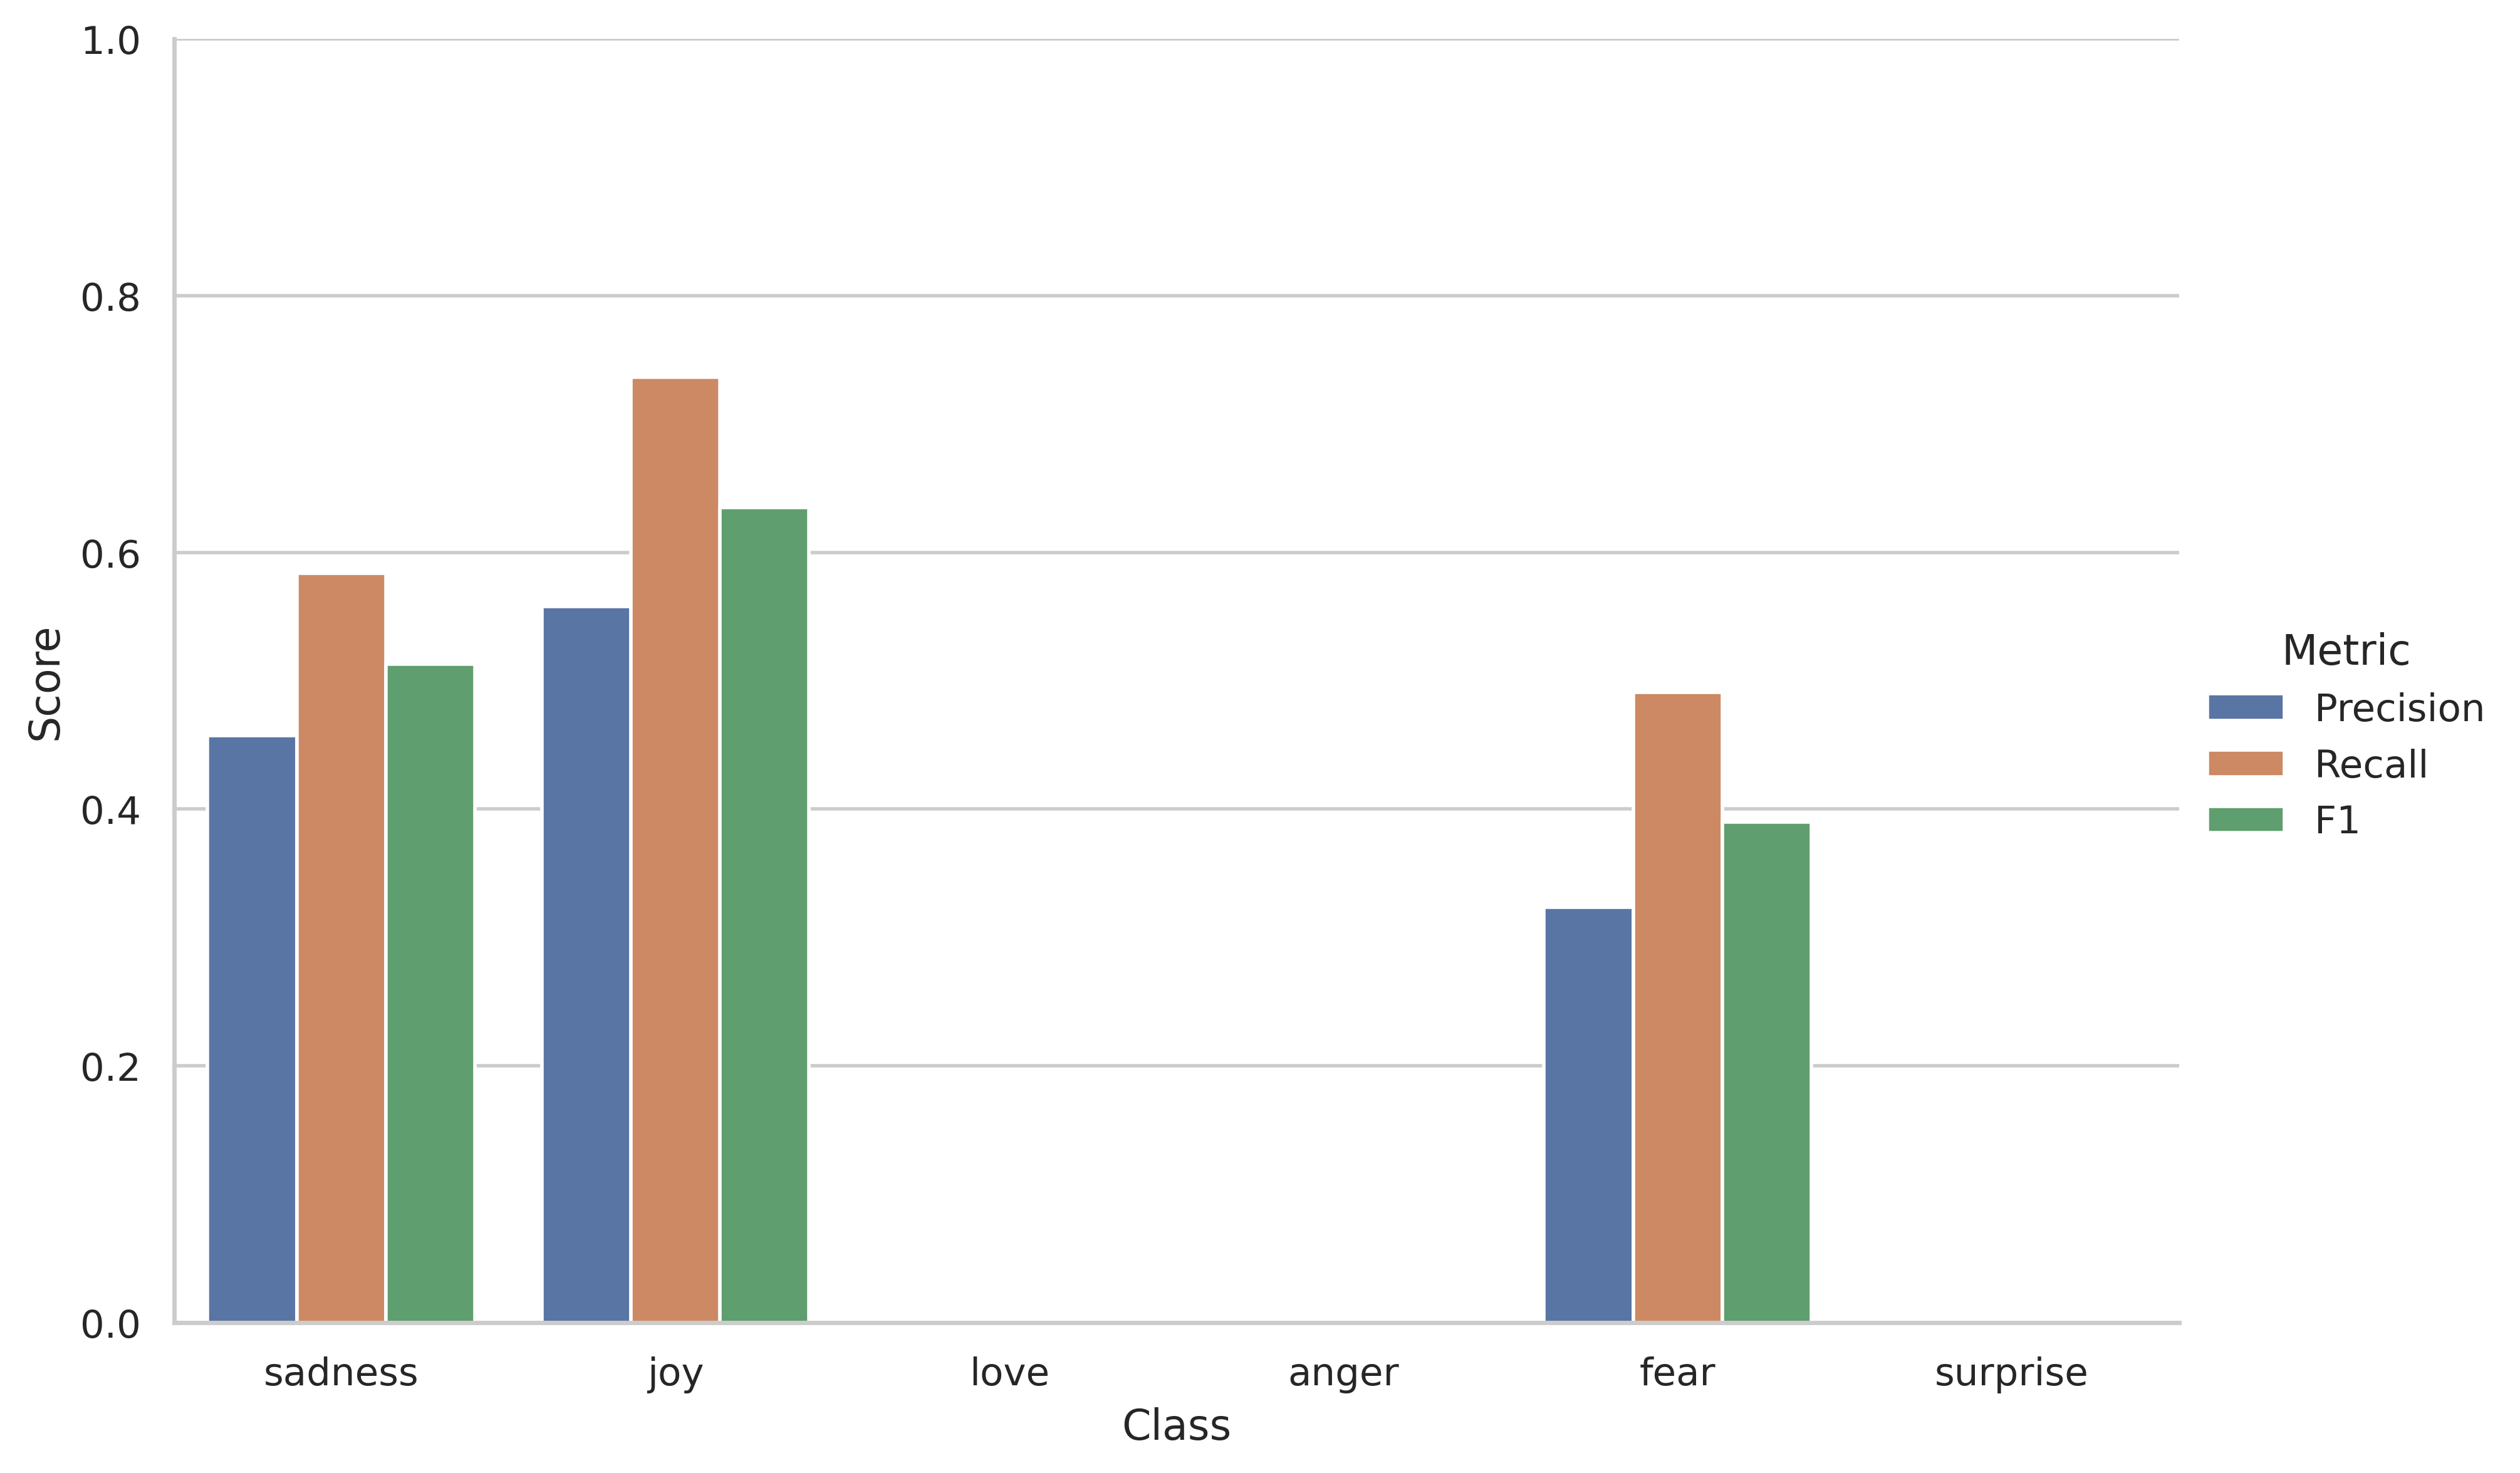
\includegraphics[width=0.6\textwidth]{img/distilbert/one_shot_light_metrics.png}
    \caption{Rappresentazione grafica delle metriche in configurazione One-Shot}
\end{figure}

\vspace{0.5cm}

\begin{figure}[H]
    \centering
    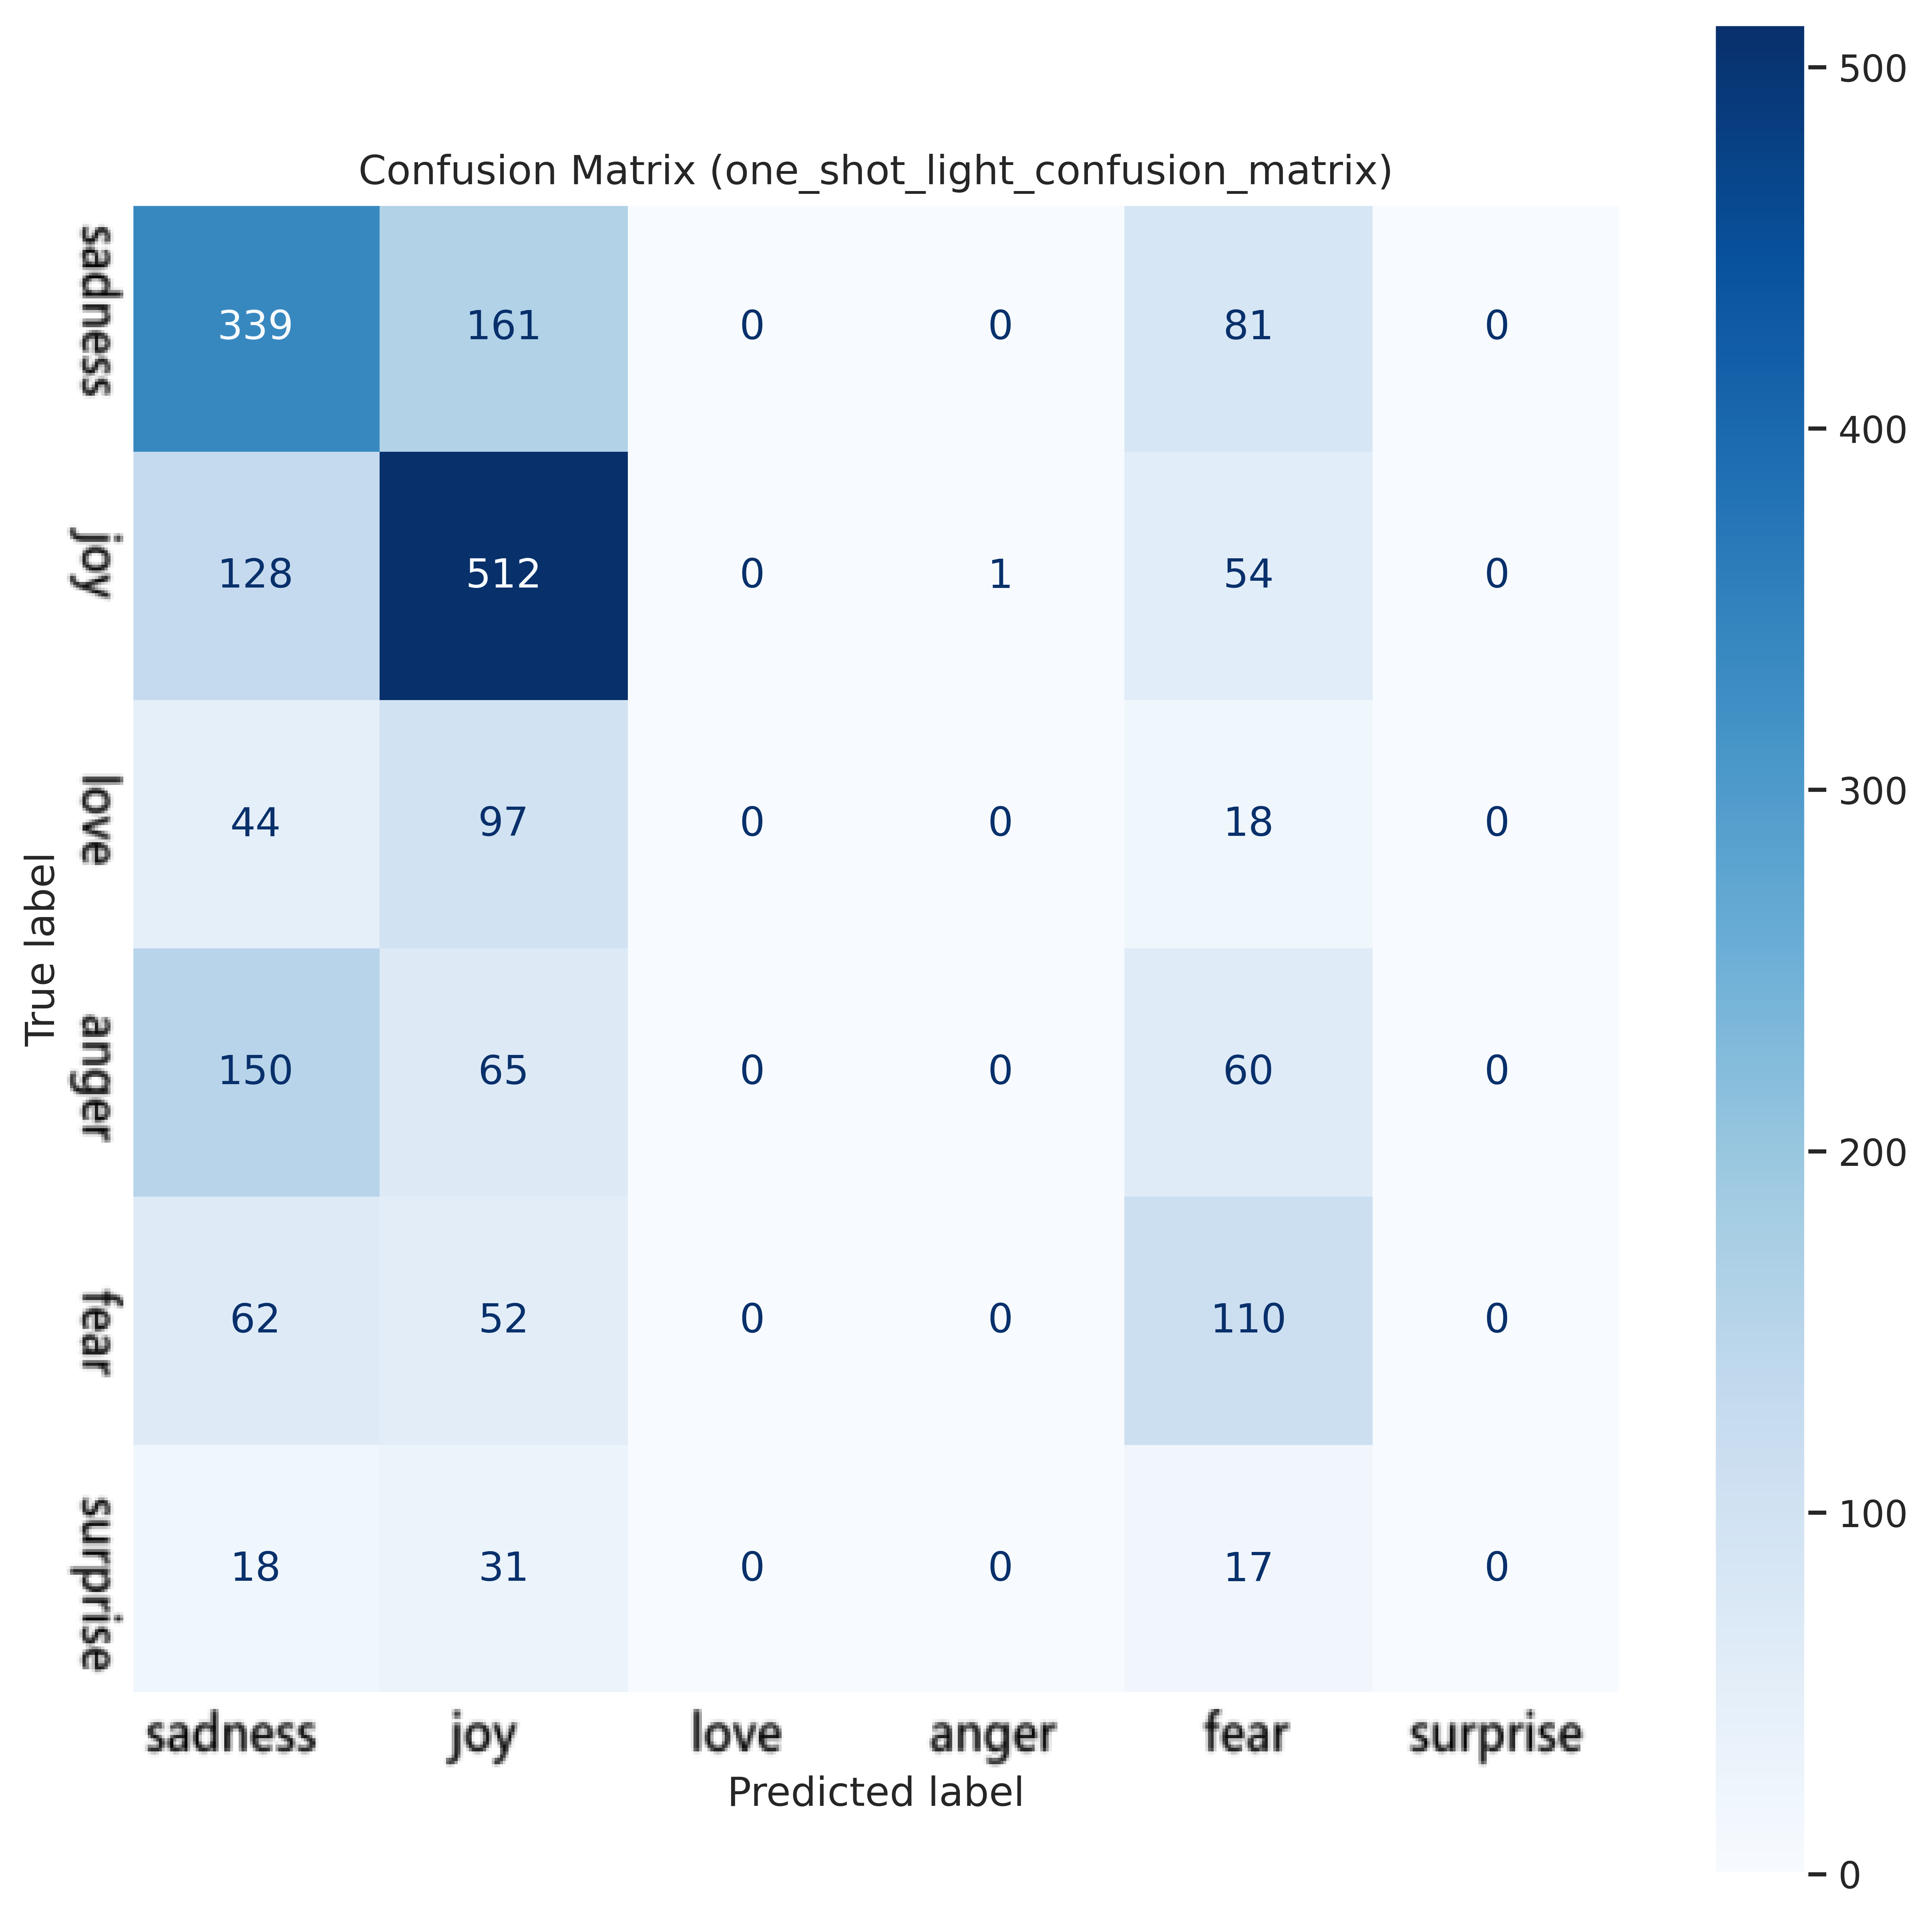
\includegraphics[width=0.6\textwidth]{img/distilbert/Confusion_Matrix_one_shot_light_confusion_matrix.png}
    \caption{Confusion matrix del modello in configurazione One-Shot}
\end{figure}

\subsubsection*{Performance Three-Shot}

\begin{table}[H]
    \centering
    \begin{tabular}{cc}
        \toprule
        Metric & Value \\
        \midrule
        Accuracy & 0.4540 \\
        \bottomrule
    \end{tabular}
    \caption{Accuracy del modello in configurazione Three-Shot}
\end{table}

\vspace{0.5cm}

\begin{table}[H]
    \centering
    \begin{tabular}{cccc}
        \toprule
        Class & Precision & Recall & F1 \\
        \midrule
        Sadness & 0.5103 & 0.3838 & 0.4381 \\
        Joy & 0.4350 & 0.9525 & 0.5972 \\
        Love & 0.0000 & 0.0000 & 0.0000 \\
        Anger & 0.0000 & 0.0000 & 0.0000 \\
        Fear & 0.5610 & 0.1027 & 0.1736 \\
        Surprise & 0.0000 & 0.0000 & 0.0000 \\
        \bottomrule
    \end{tabular}
    \caption{Metriche di precision, recall e F1 per classe in configurazione Three-Shot}
\end{table}

\vspace{0.5cm}

\begin{figure}[H]
    \centering
    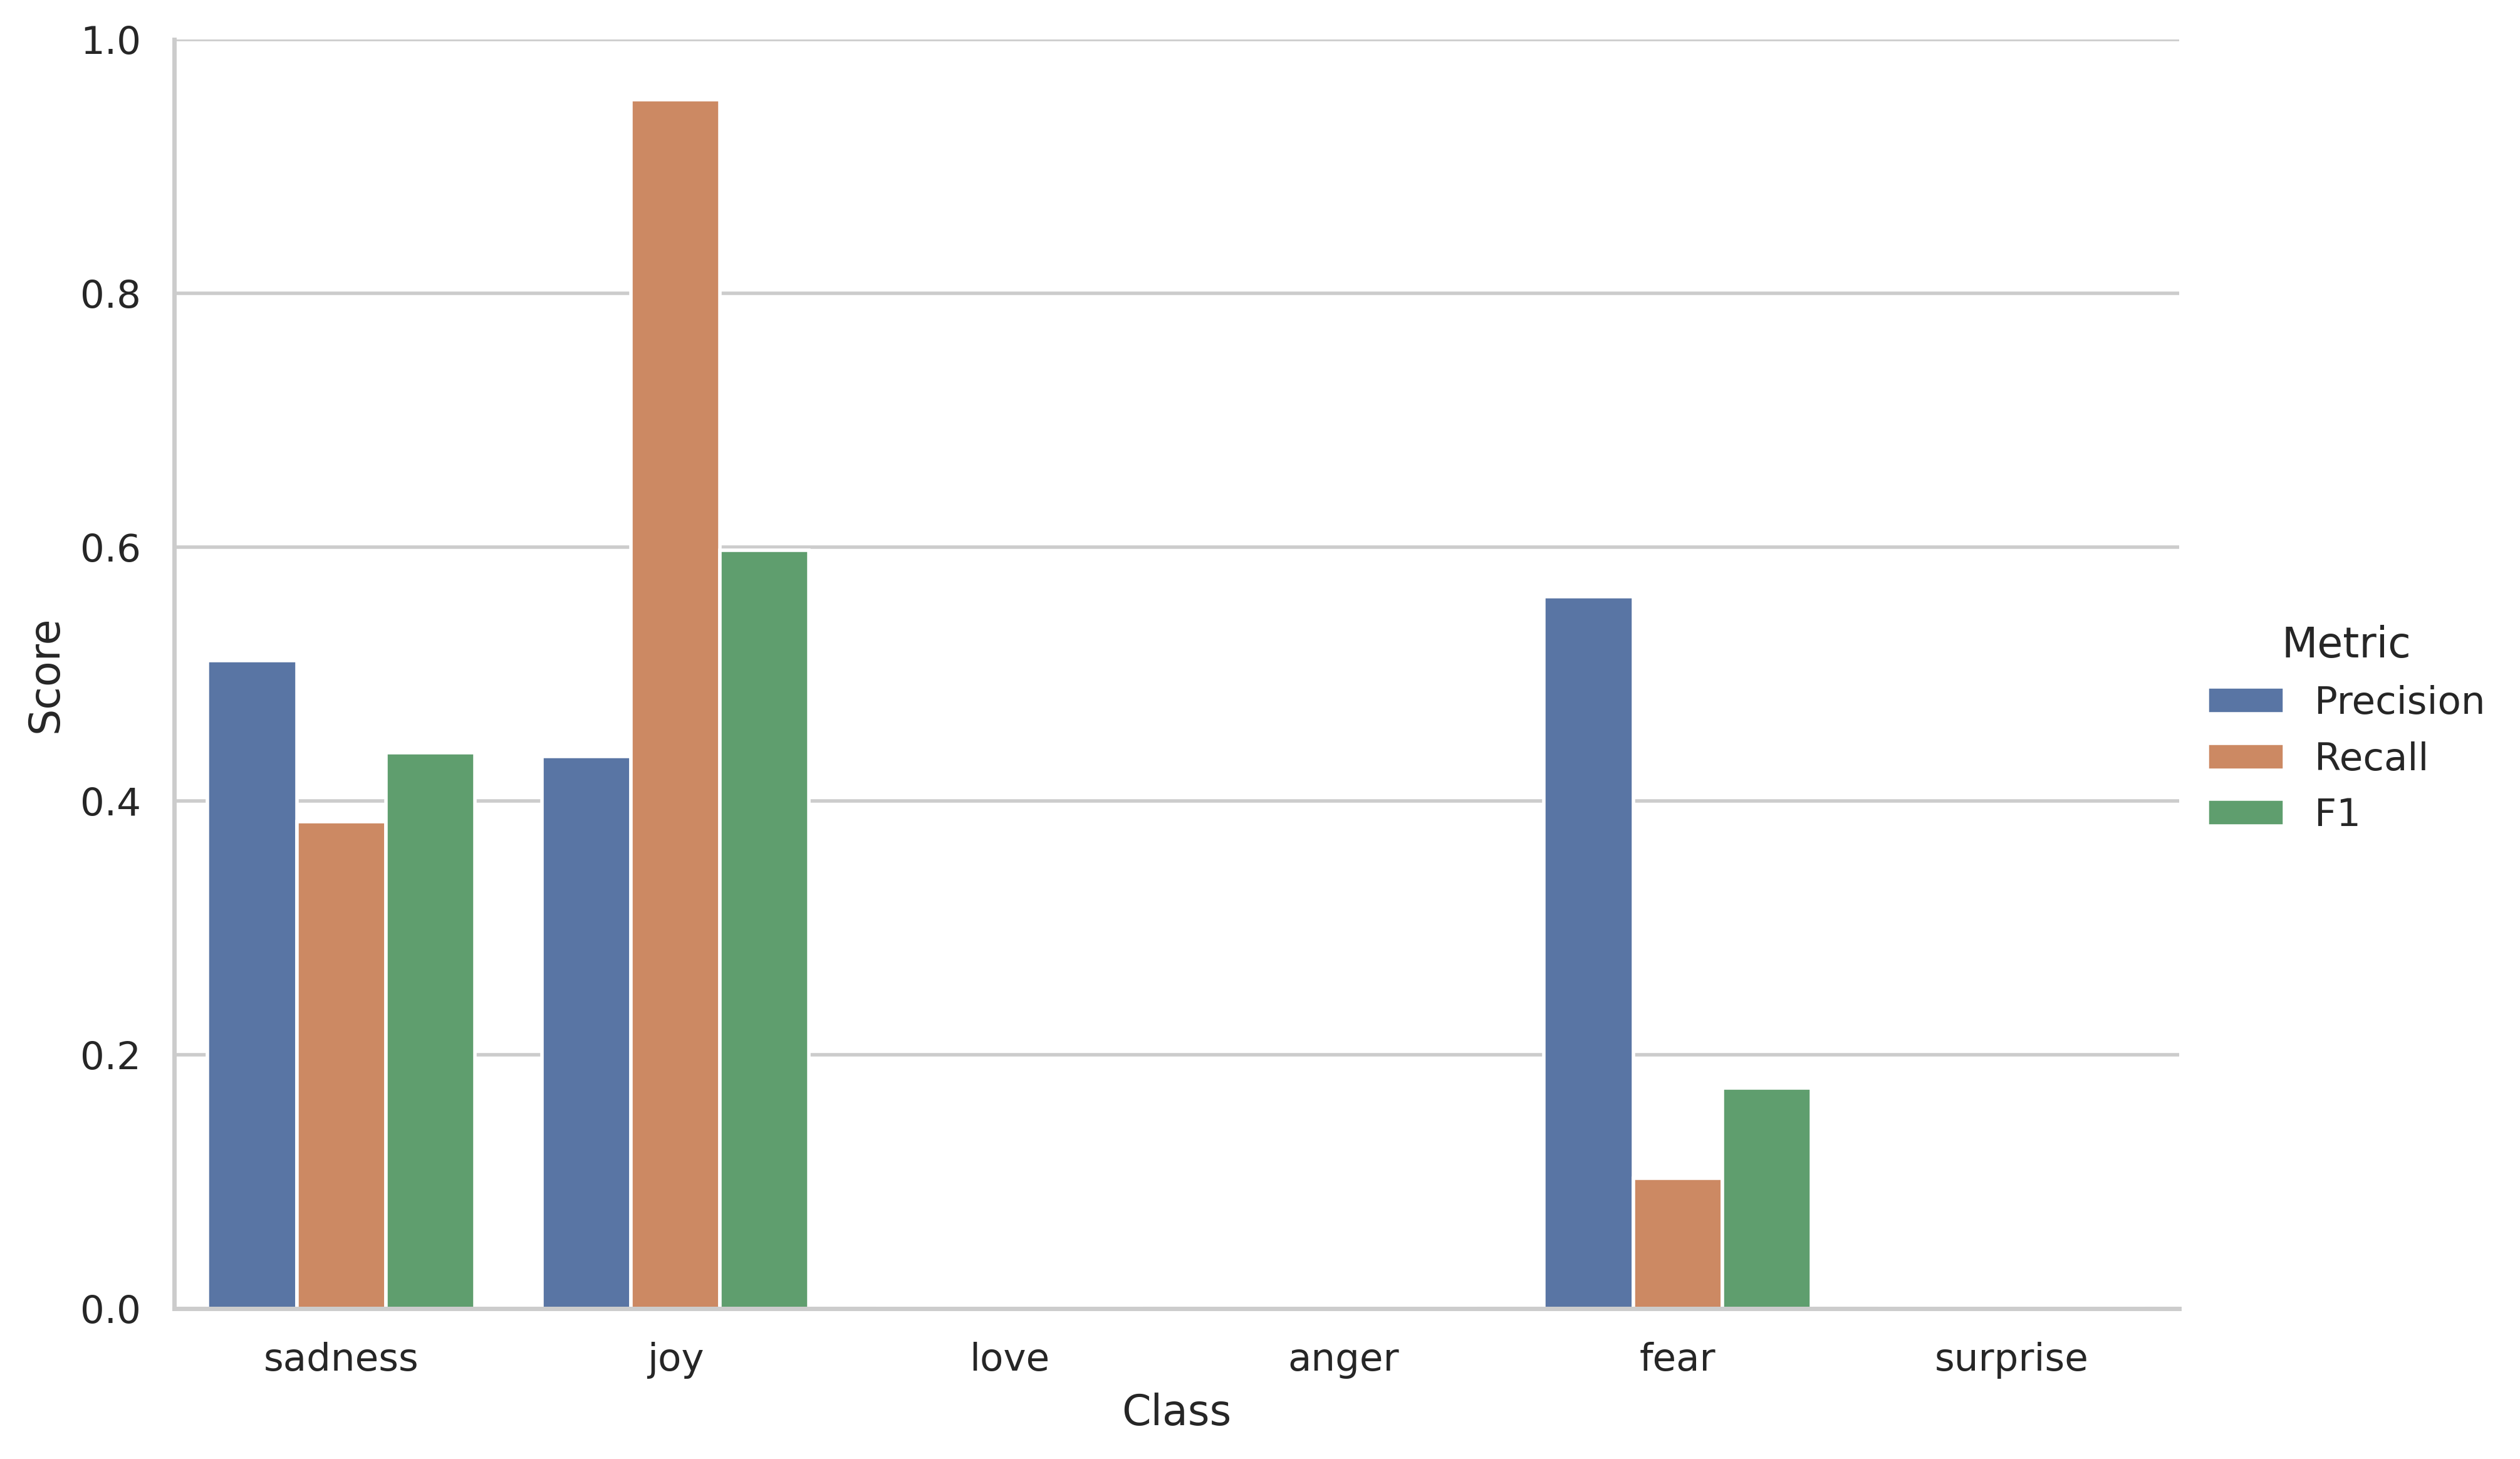
\includegraphics[width=0.6\textwidth]{img/distilbert/three_shot_light_metrics.png}
    \caption{Rappresentazione grafica delle metriche in configurazione Three-Shot}
\end{figure}

\vspace{0.5cm}

\begin{figure}[H]
    \centering
    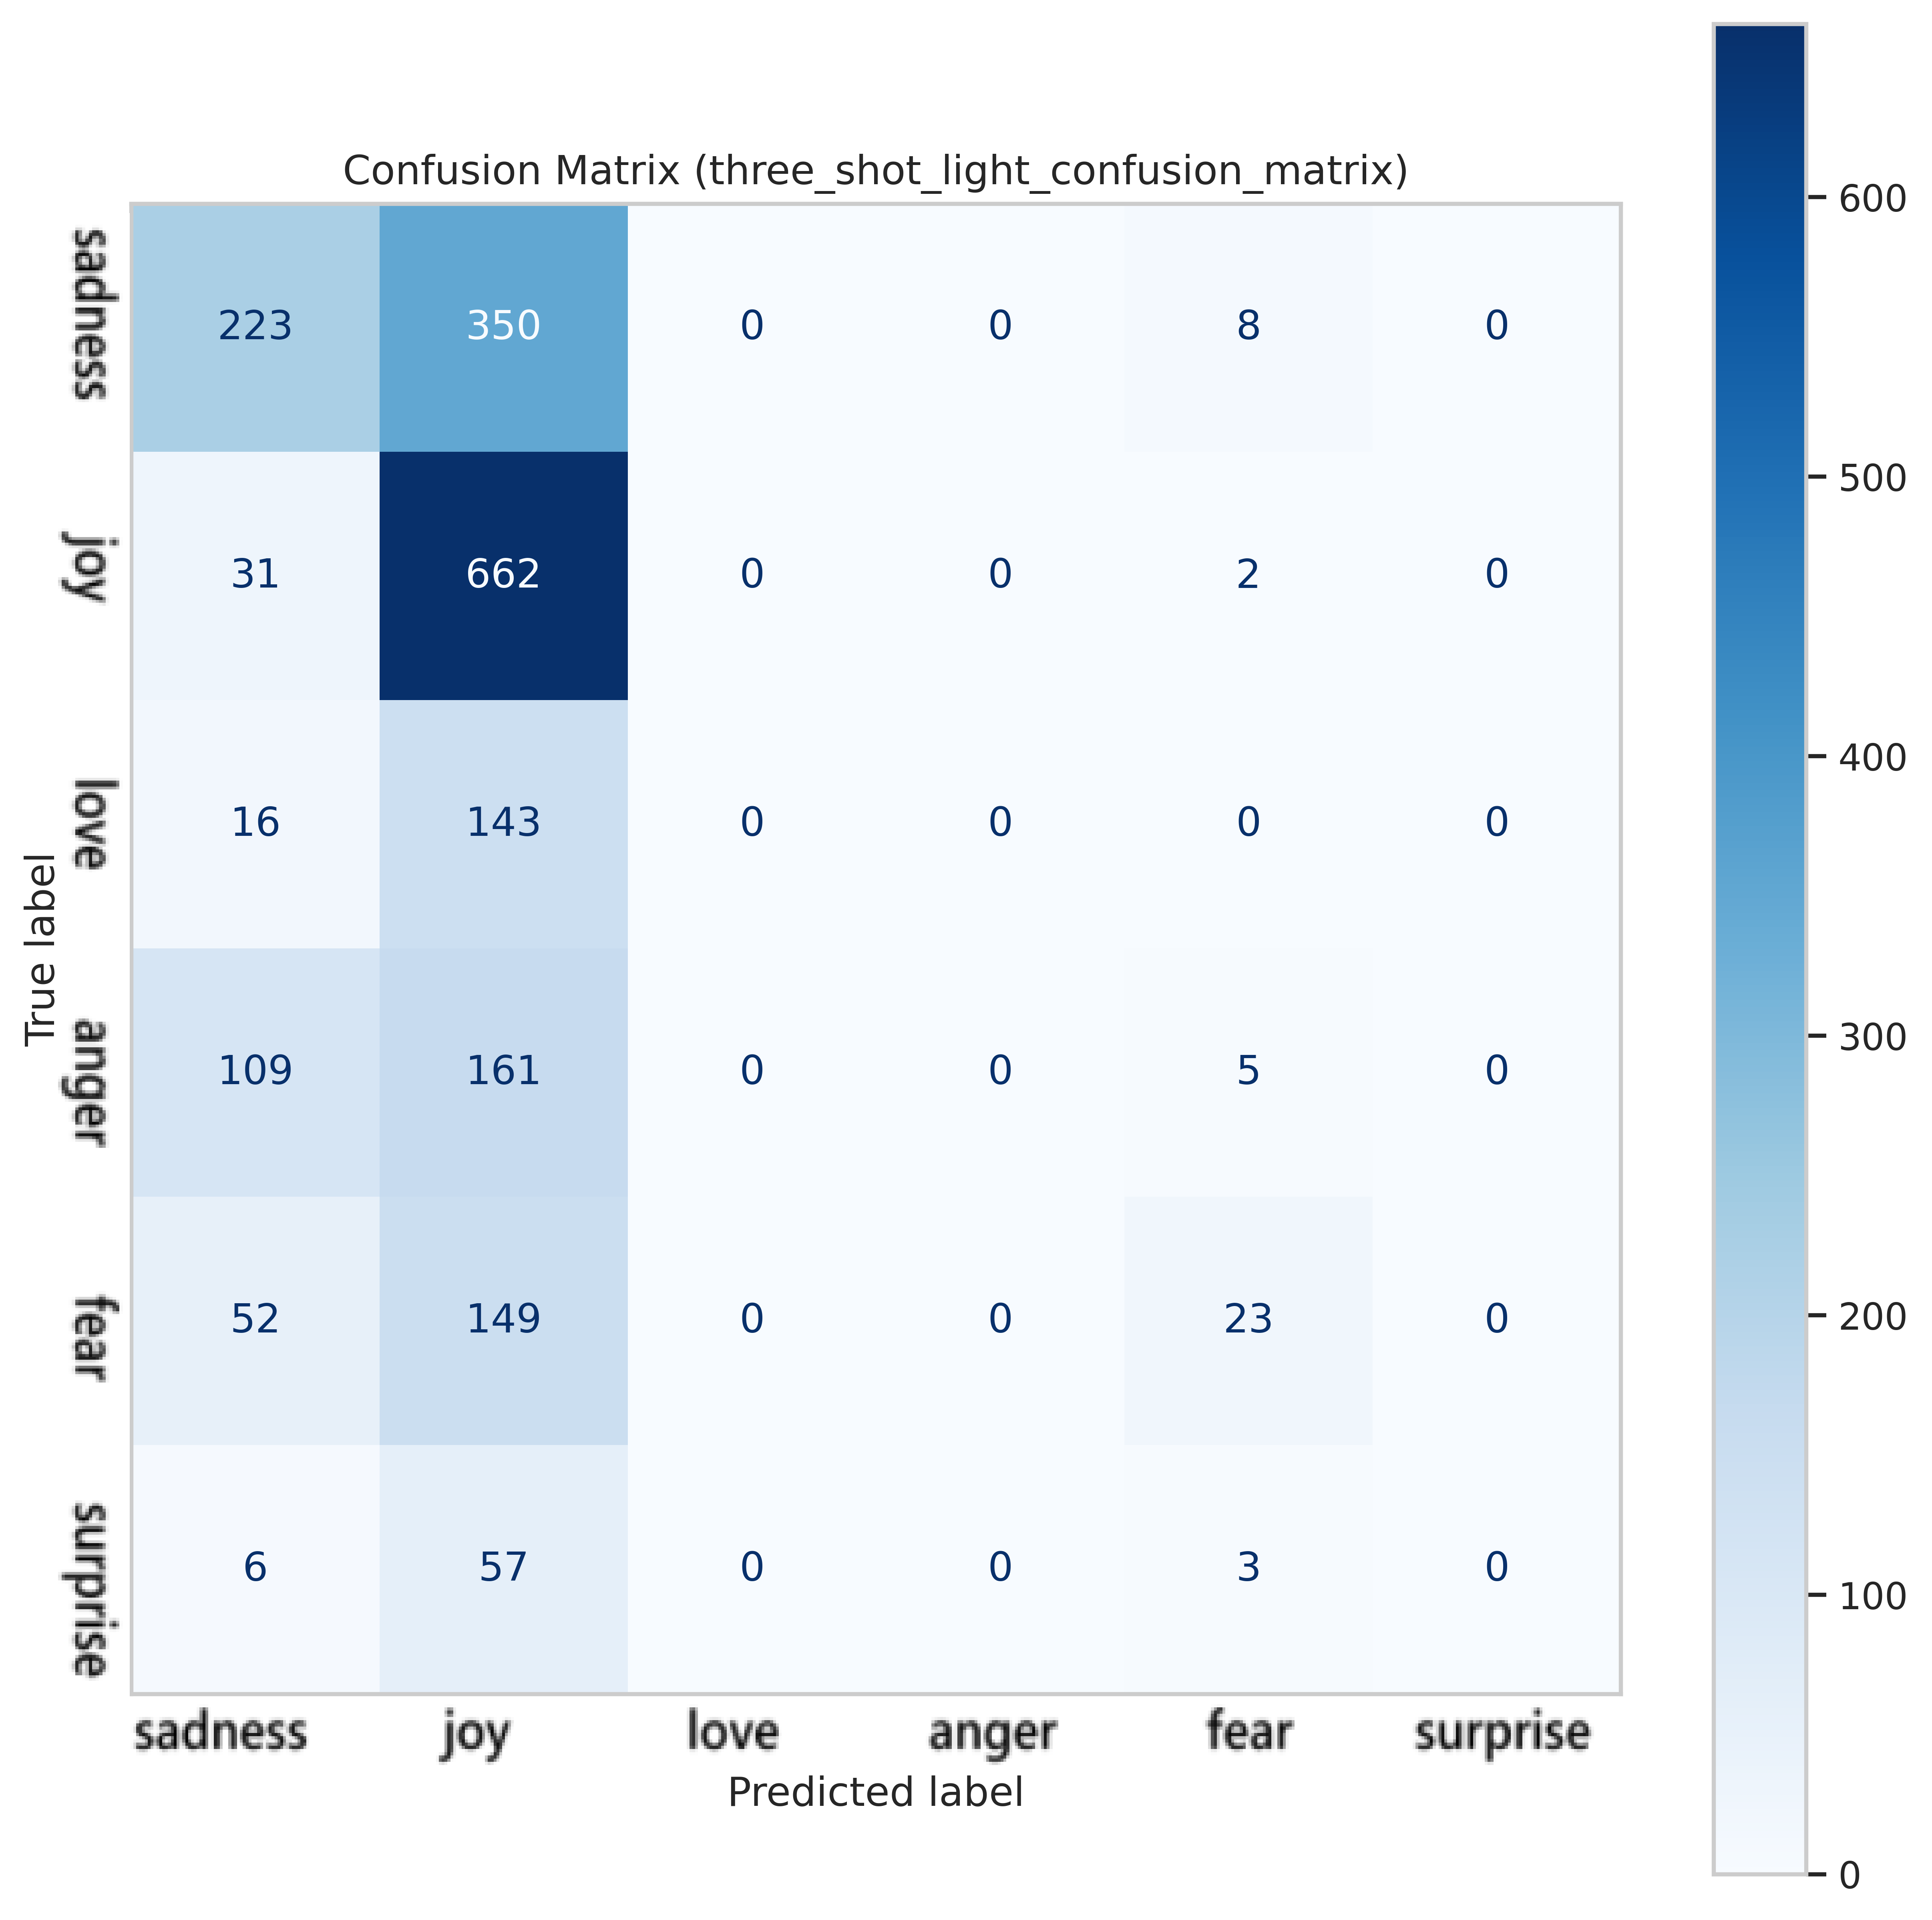
\includegraphics[width=0.6\textwidth]{img/distilbert/Confusion_Matrix_three_shot_light_confusion_matrix.png}
    \caption{Confusion matrix del modello in configurazione Three-Shot}
\end{figure}

\subsubsection*{Performance Five-Shot}

\begin{table}[H]
    \centering
    \begin{tabular}{cc}
        \toprule
        Metric & Value \\
        \midrule
        Accuracy & 0.4730 \\
        \bottomrule
    \end{tabular}
    \caption{Accuracy del modello in configurazione Five-Shot}
\end{table}

\vspace{0.5cm}

\begin{table}[H]
    \centering
    \begin{tabular}{cccc}
        \toprule
        Class & Precision & Recall & F1 \\
        \midrule
        Sadness & 0.4152 & 0.7917 & 0.5447 \\
        Joy & 0.6433 & 0.5554 & 0.5961 \\
        Love & 0.0000 & 0.0000 & 0.0000 \\
        Anger & 0.0000 & 0.0000 & 0.0000 \\
        Fear & 0.3425 & 0.4464 & 0.3876 \\
        Surprise & 0.0000 & 0.0000 & 0.0000 \\
        \bottomrule
    \end{tabular}
    \caption{Metriche di precision, recall e F1 per classe in configurazione Five-Shot}
\end{table}

\vspace{0.5cm}

\begin{figure}[H]
    \centering
    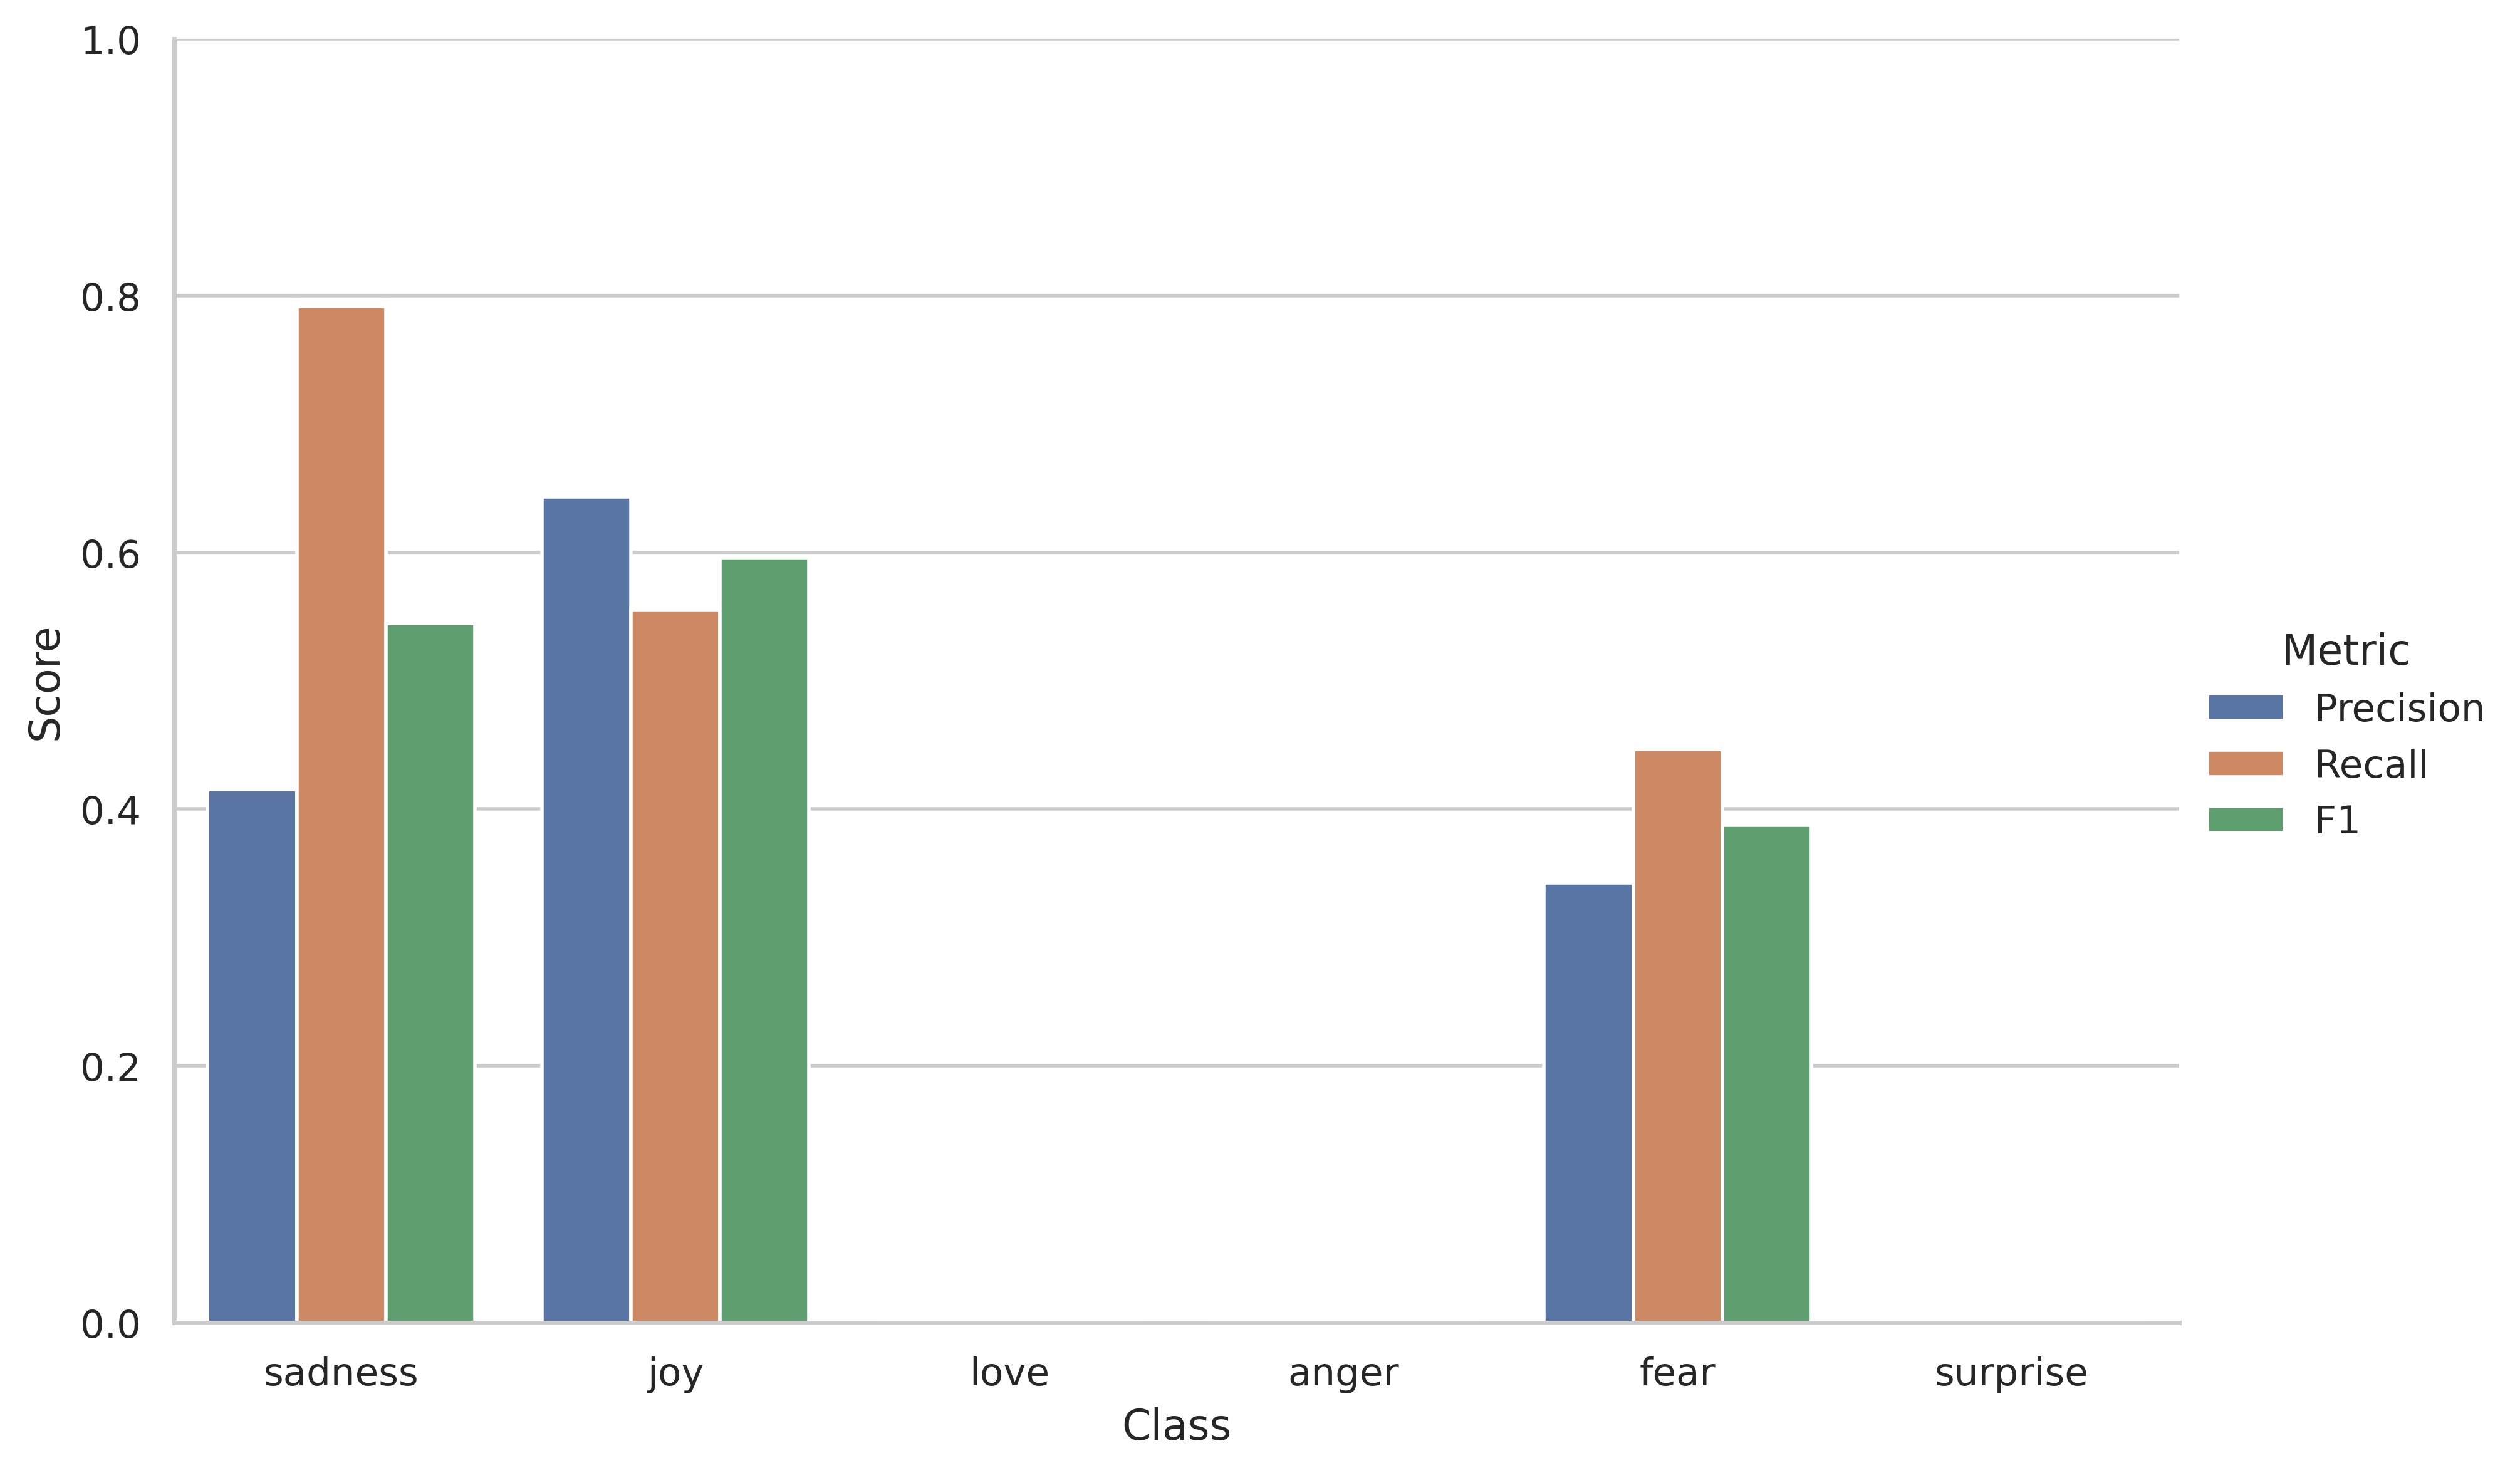
\includegraphics[width=0.6\textwidth]{img/distilbert/five_shot_light_metrics.png}
    \caption{Rappresentazione grafica delle metriche in configurazione Five-Shot}
\end{figure}

\vspace{0.5cm}

\begin{figure}[H]
    \centering
    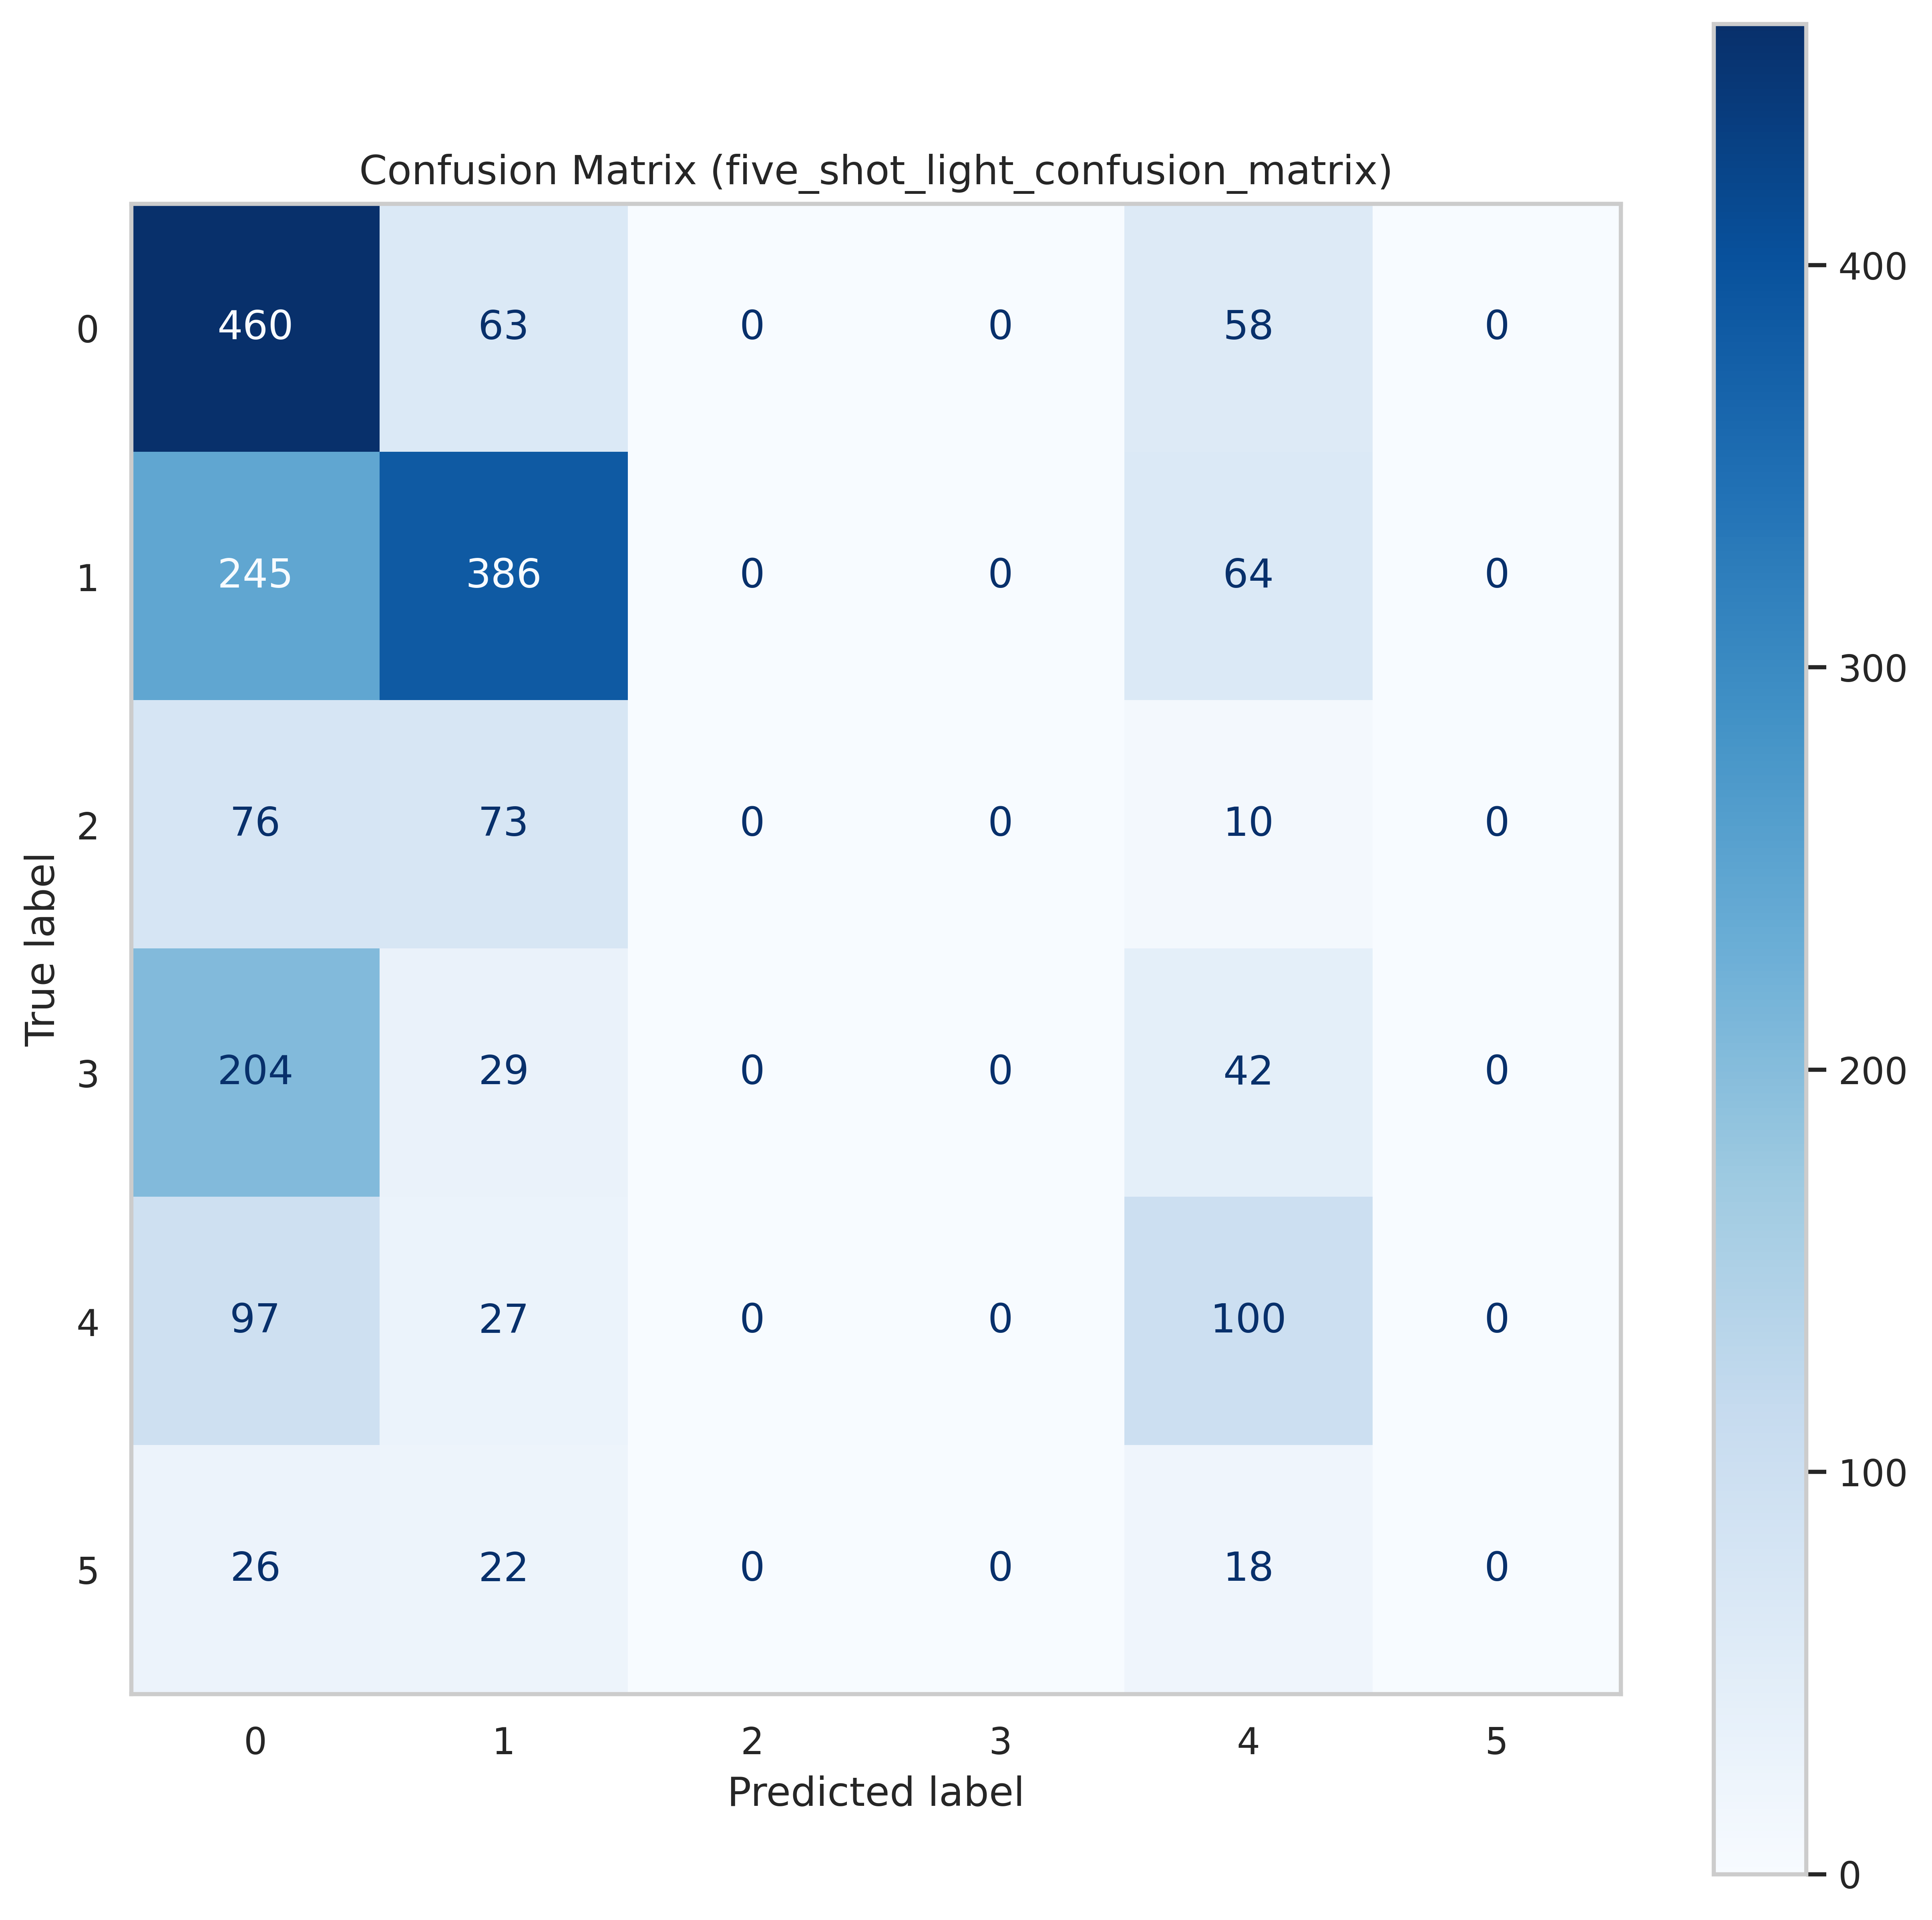
\includegraphics[width=0.6\textwidth]{img/distilbert/Confusion_Matrix_five_shot_light_confusion_matrix.png}
    \caption{Confusion matrix del modello in configurazione Five-Shot}
\end{figure}

\subsubsection*{Confronto Performance In-Context Learning}

In questa sezione si confrontano le performance dei vari gradi di inContext, ma per rendere il confronto più comprensibile, si è scelto di restringere le metriche di valutazione a F1 e Accuracy.

\begin{figure}[H]
    \centering
    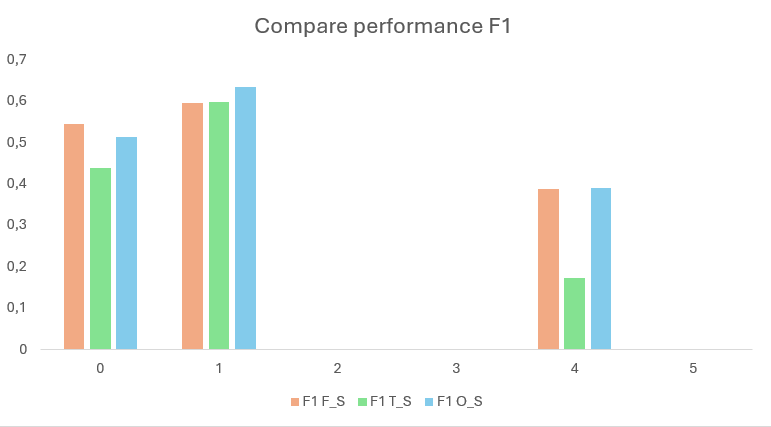
\includegraphics[width=0.8\textwidth]{img/distilbert/compare performance f1.png}
    \caption{Confronto F1-score}
\end{figure}

Il grafico confronta l’F1-score ottenuto nelle diverse configurazioni sperimentali (Five Shot, Three Shot e One Shot) per ciascuna classe. Si osserva che la classe Joy mantiene le prestazioni migliori in tutte le configurazioni, con valori di F1 prossimi a 0.6, confermandosi la categoria più facilmente discriminabile dal modello.

La classe Sadness mostra prestazioni intermedie, con un miglioramento nella configurazione Five Shot rispetto alle altre. La classe Fear, invece, presenta valori sensibilmente più bassi, evidenziando una maggiore difficoltà del modello nel riconoscere correttamente tale categoria.

Nel complesso, le prestazioni risultano sbilanciate tra le classi: alcune categorie vengono apprese in modo più efficace, mentre altre rimangono più problematiche.

\begin{figure}[H]
    \centering
    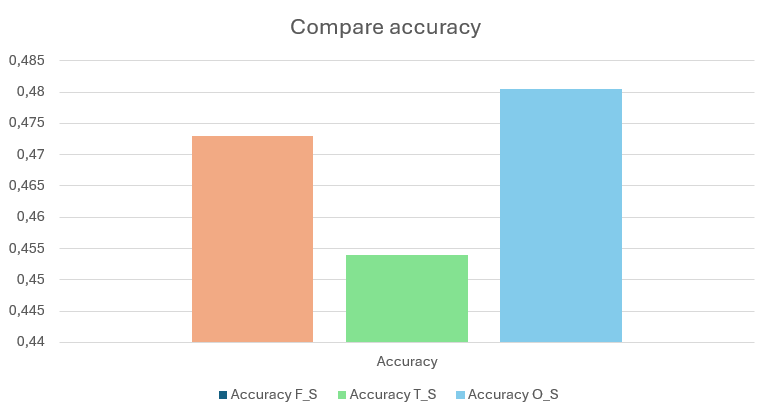
\includegraphics[width=0.8\textwidth]{img/distilbert/compare accuracy.png}
    \caption{Confronto Accuracy}
\end{figure}

Il grafico evidenzia che l’accuracy globale non cresce in modo monotono all’aumentare degli shot: si osserva una diminuzione nel three-shot rispetto all’one-shot, seguita da un miglioramento nel five-shot. Tuttavia, i valori rimangono contenuti, coerentemente con la forte polarizzazione del modello verso una singola classe. L’accuracy risulta quindi influenzata dallo sbilanciamento delle predizioni, non riflettendo un apprendimento uniforme su tutte le classi.

\subsubsection*{Performance Fine-tuning Completo}

In questa sezione vengono presentate le prestazioni del modello sul test set a seguito del processo di fine-tuning completo.

\begin{table}[H]
    \centering
    \begin{tabular}{cc}
        \toprule
        Metric & Value \\
        \midrule
        Accuracy & 0.9260 \\
        \bottomrule
    \end{tabular}
    \caption{Accuracy del modello dopo Fine-tuning Completo}
\end{table}

\vspace{0.5cm}

\begin{table}[H]
    \centering
    \begin{tabular}{cccc}
        \toprule
        Class & Precision & Recall & F1     \\
        \midrule
        Sadness     & 0.9621    & 0.9604 & 0.9612 \\
        Joy     & 0.9406    & 0.9568 & 0.9486 \\
        Love     & 0.8553    & 0.8176 & 0.8360 \\
        Anger     & 0.9211    & 0.9211 & 0.9211 \\
        Fear     & 0.8692    & 0.9196 & 0.8937 \\
        Surprise     & 0.8163    & 0.6061 & 0.6957 \\
        \bottomrule
    \end{tabular}
    \caption{Metriche di precision, recall e F1 per classe dopo Fine-tuning Completo}
\end{table}

\vspace{0.5cm}

\begin{figure}[H]
    \centering
    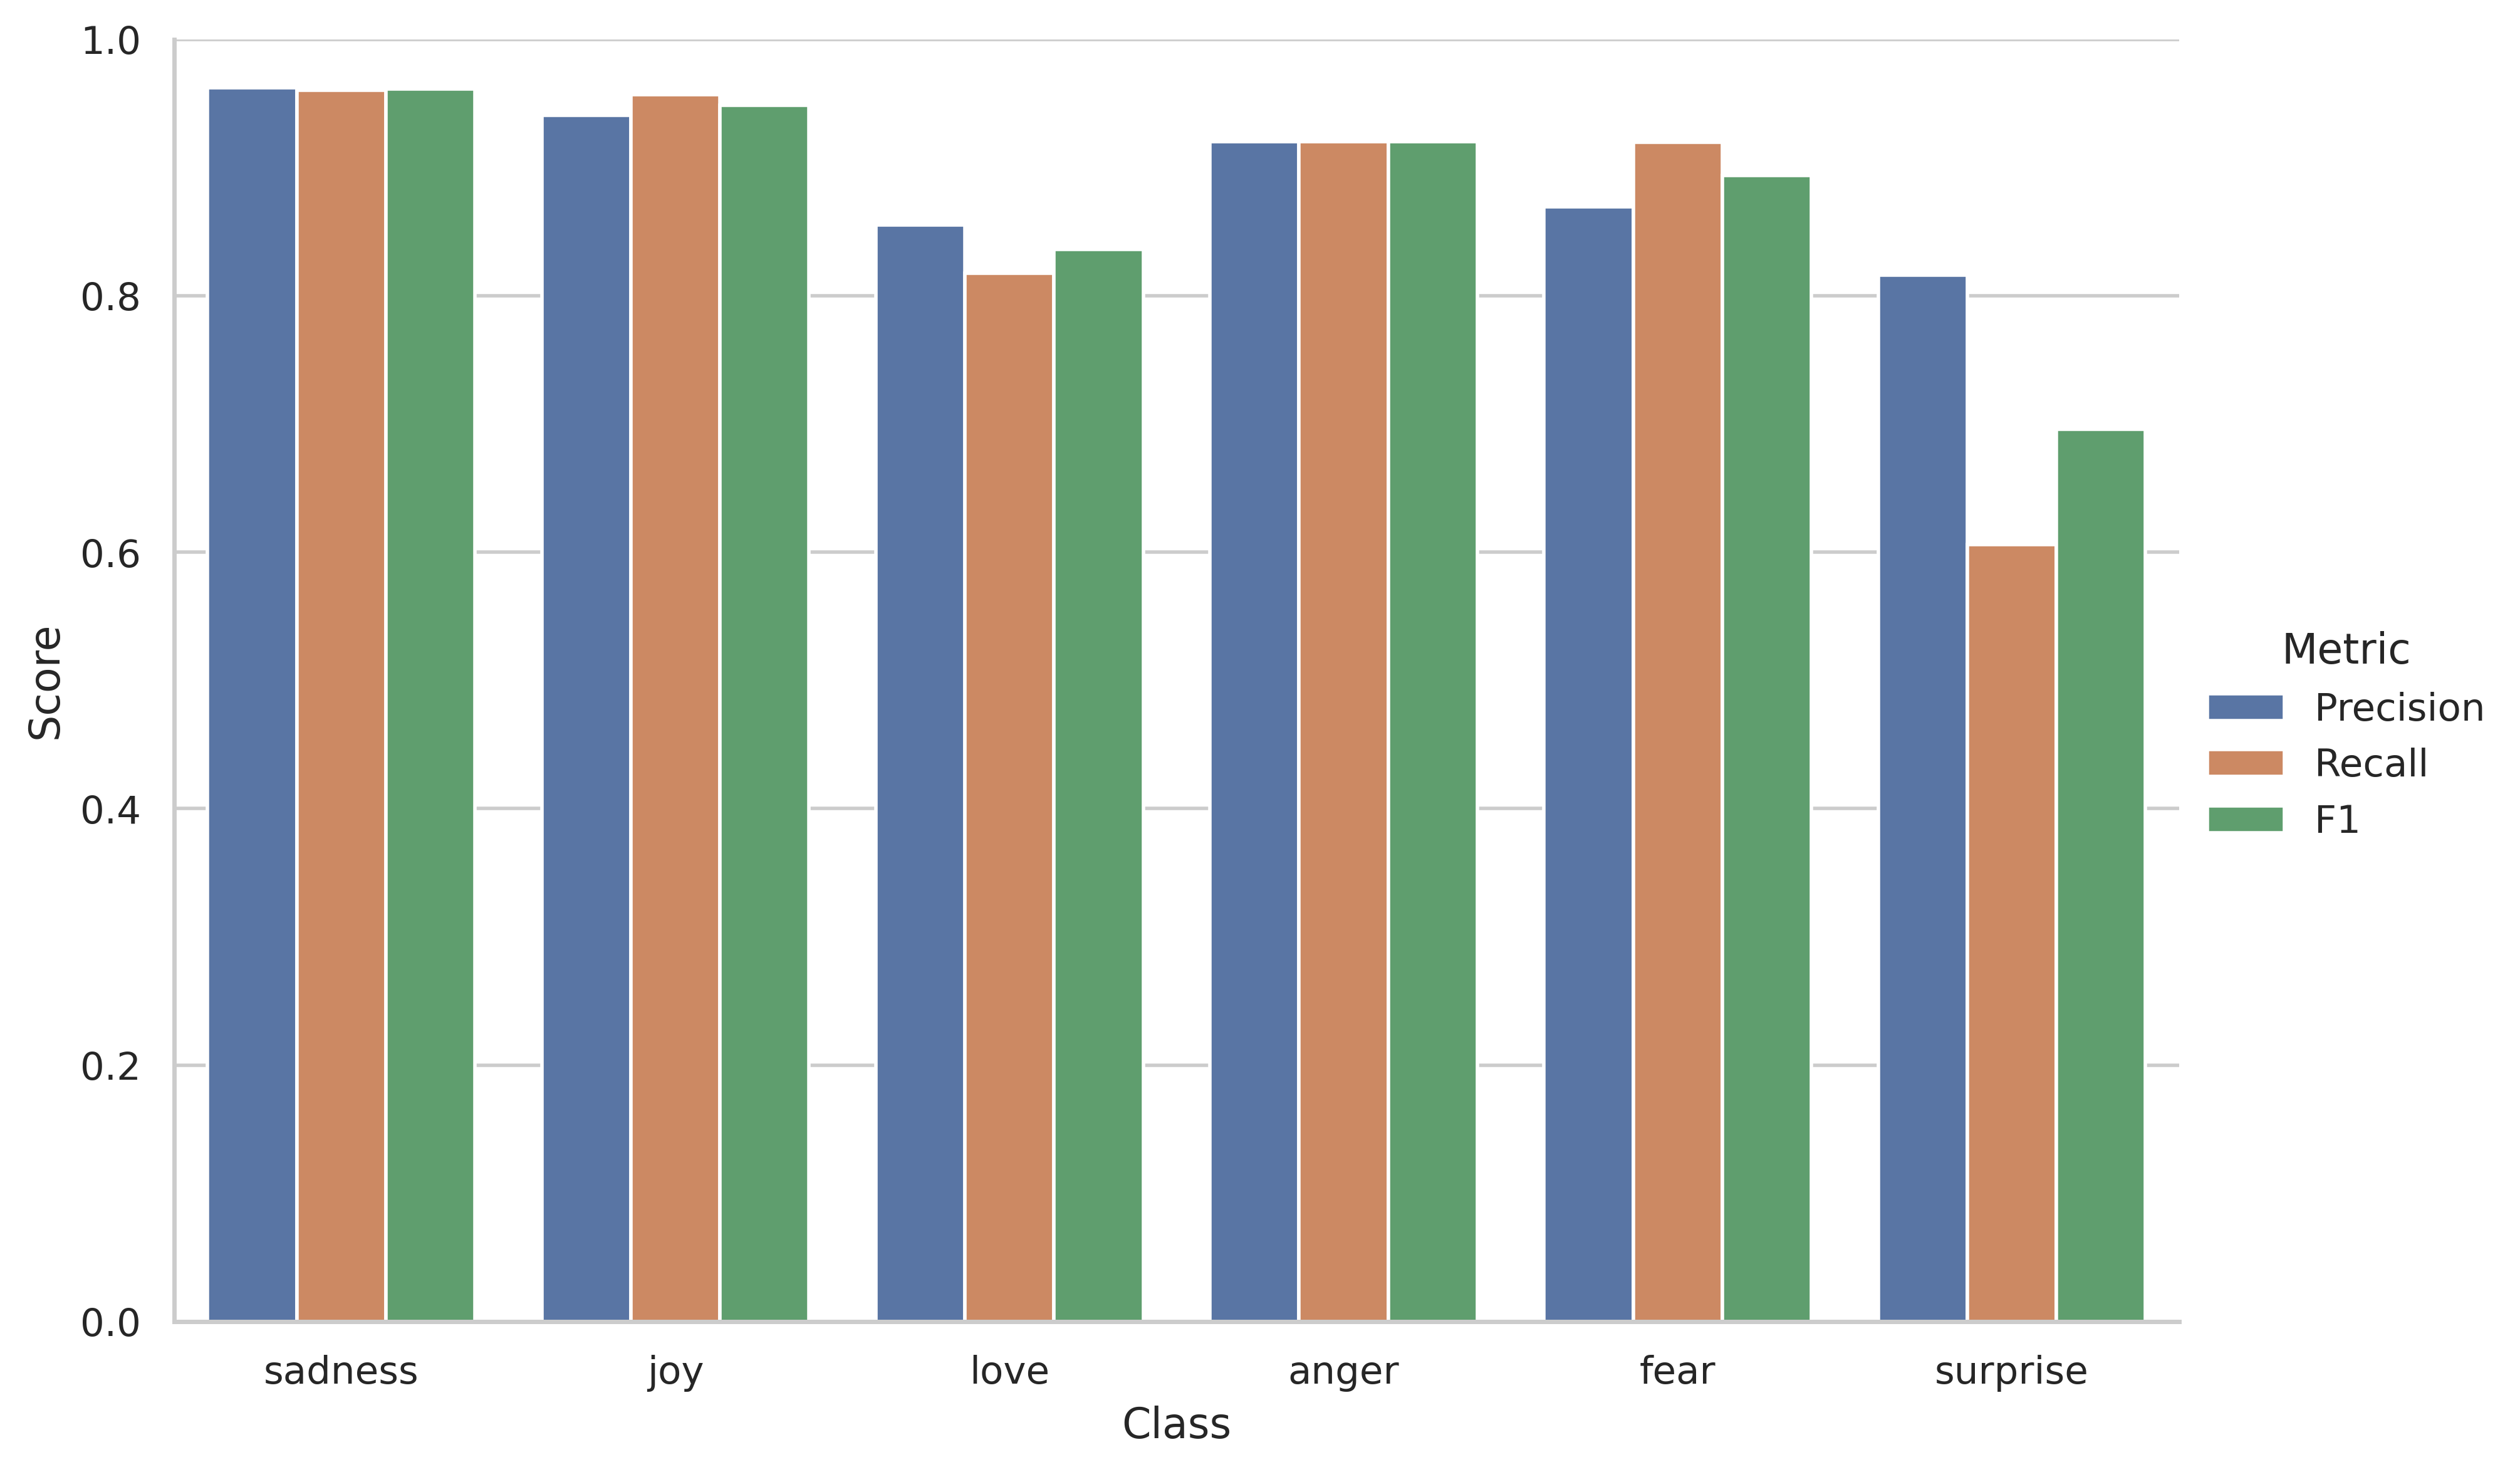
\includegraphics[width=0.8\textwidth]{img/distilbert/complete_ft_test_metrics.png}
    \caption{Rappresentazione grafica delle metriche dopo Fine-tuning Completo}
\end{figure}

Il grafico mostra Precision, Recall e F1-score per ciascuna classe emotiva dopo il fine-tuning completo del modello. Le prestazioni risultano complessivamente elevate e bilanciate per la maggior parte delle classi. In particolare, sadness, joy e anger presentano valori prossimi a 0.95–0.97, indicando un’elevata capacità del modello di identificare correttamente tali categorie con un buon equilibrio tra precisione e richiamo.

Anche fear e love mostrano risultati solidi, sebbene con una lieve variabilità tra precision e recall. La classe surprise risulta invece la più complessa da classificare, con una riduzione più marcata soprattutto nel recall, suggerendo una maggiore difficoltà del modello nel riconoscere tutti i casi appartenenti a questa categoria.

Nel complesso, il fine-tuning completo consente al modello di apprendere rappresentazioni discriminative efficaci, garantendo performance elevate e relativamente omogenee tra le diverse classi, con limitate criticità concentrate principalmente sulla classe surprise.

\vspace{0.5cm}

\begin{figure}[H]
    \centering
    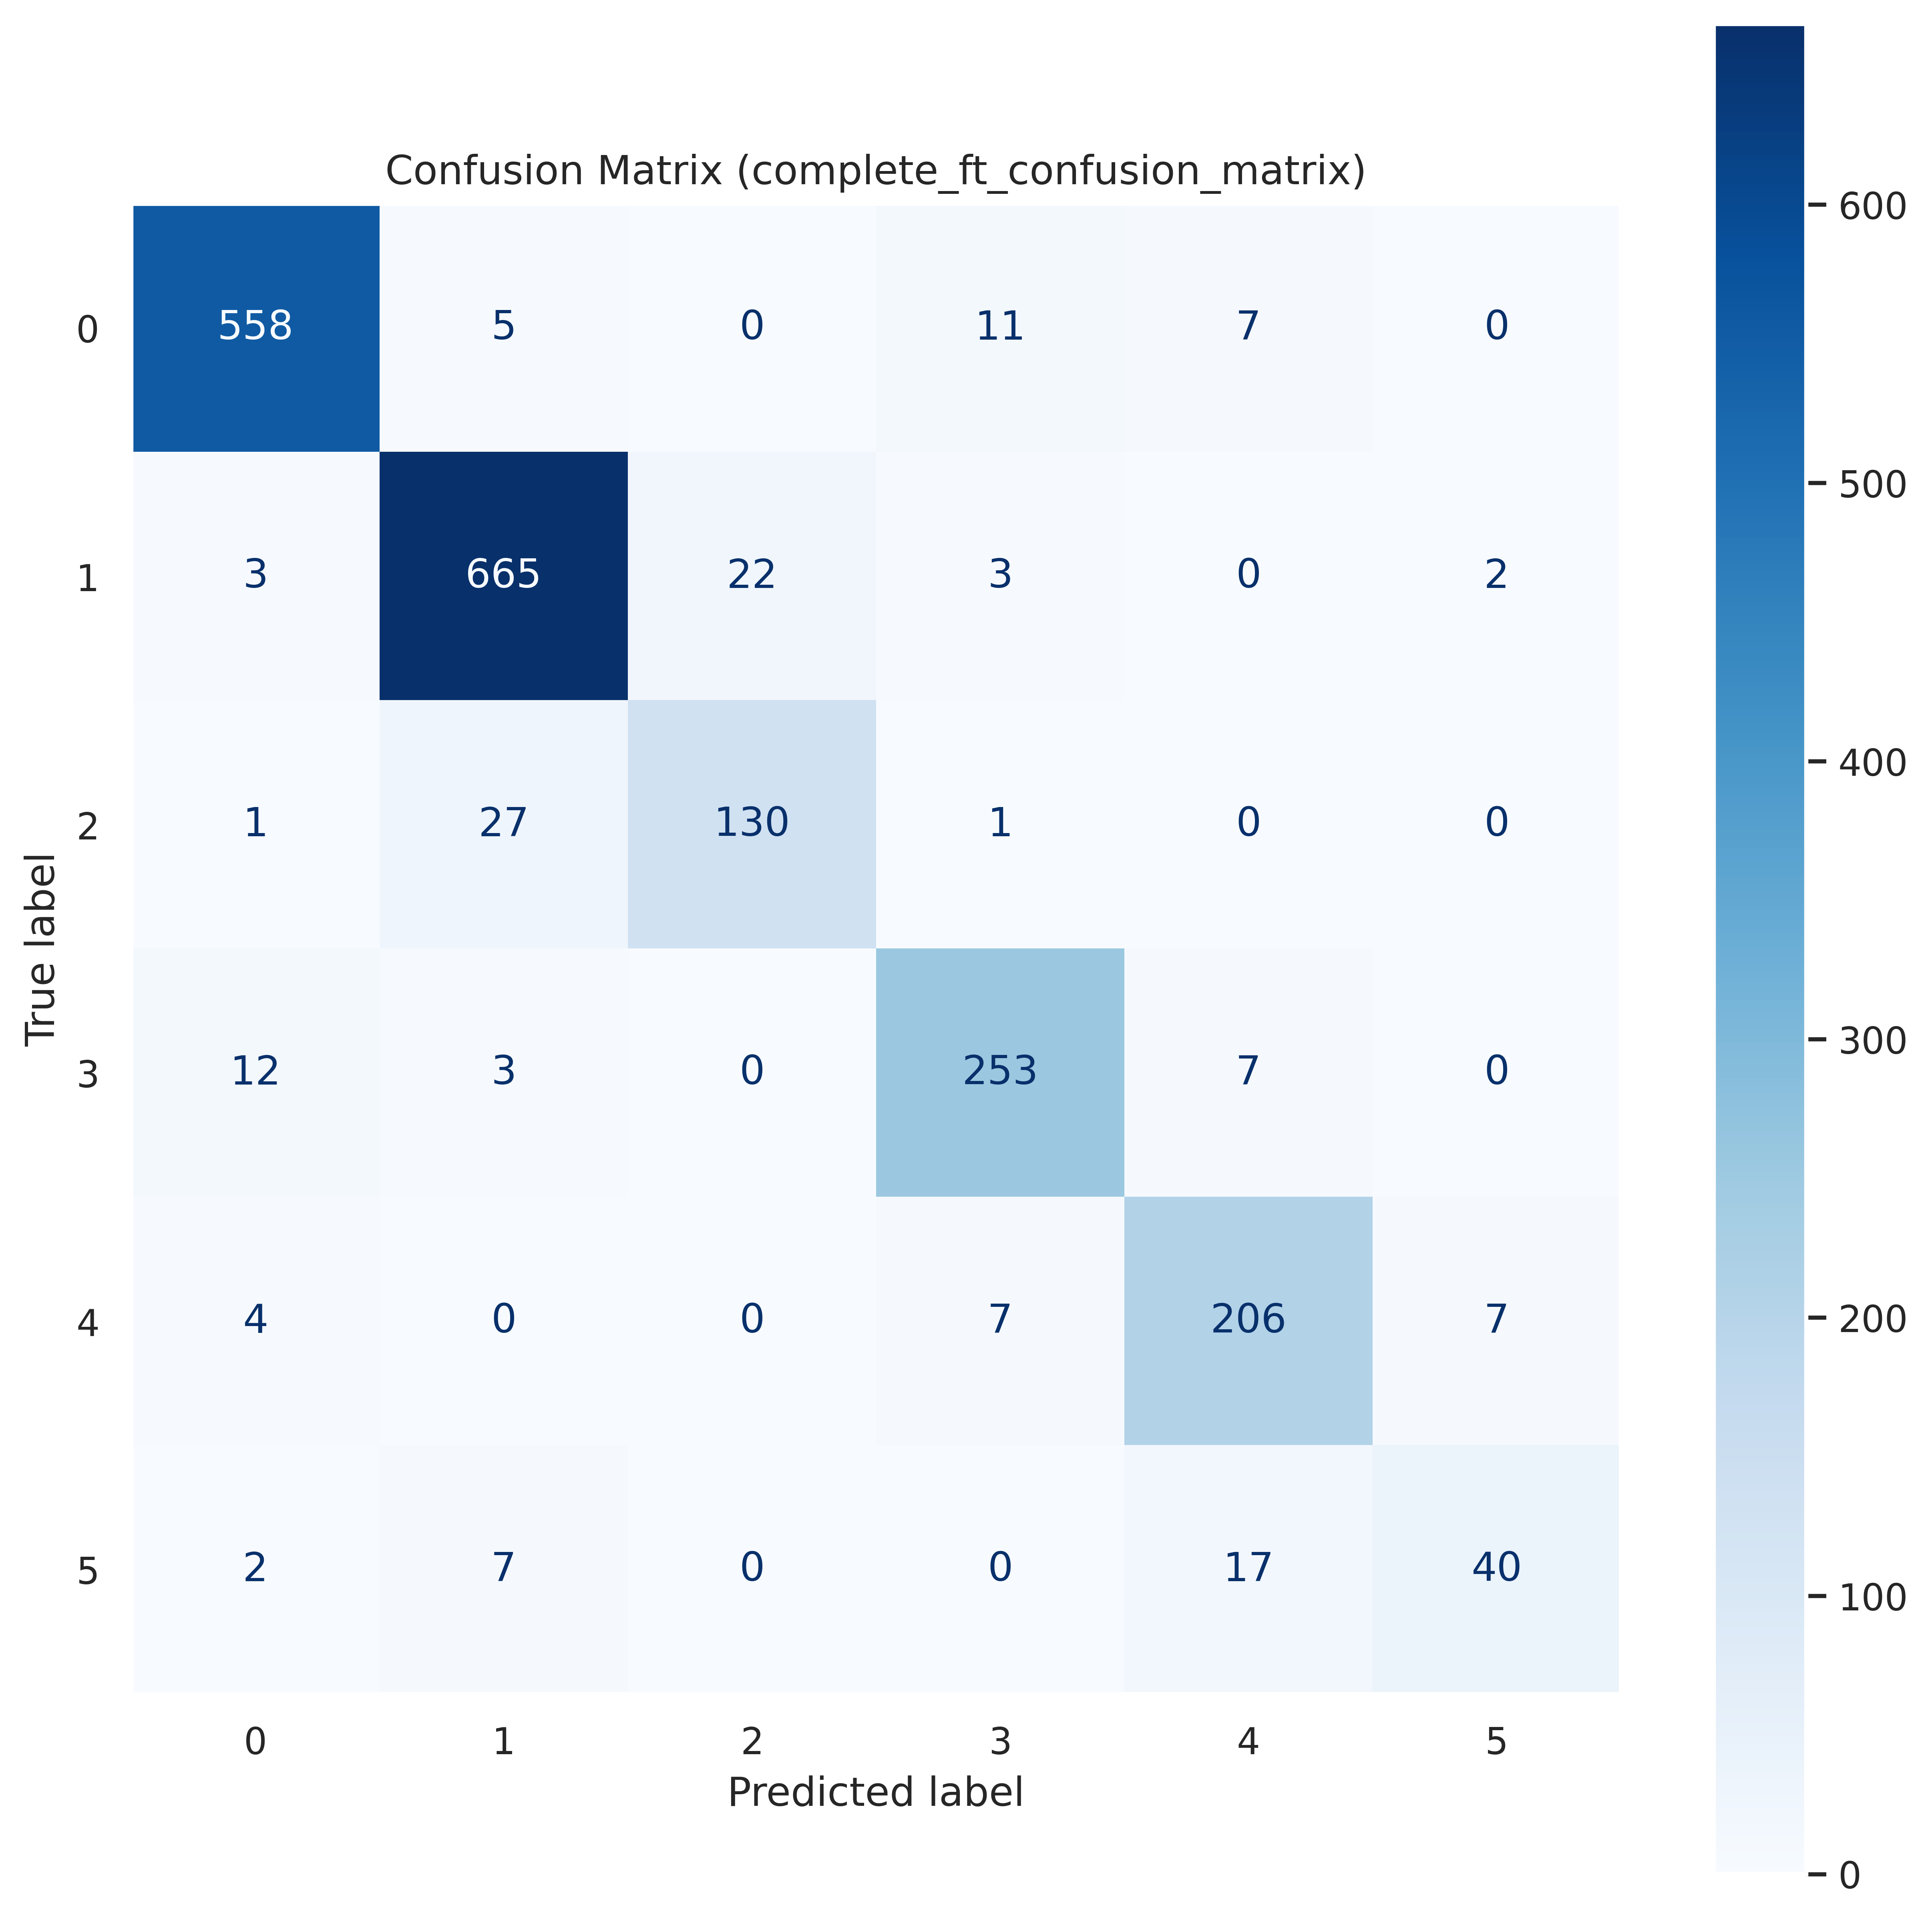
\includegraphics[width=0.8\textwidth]{img/distilbert/Confusion_Matrix_complete_ft_confusion_matrix.png}
    \caption{Confusion matrix del modello dopo Fine-tuning Completo}
\end{figure}

La matrice di confusione evidenzia le prestazioni del modello nella classificazione delle 6 classi. I valori più elevati si trovano lungo la diagonale principale, indicando un buon numero di predizioni corrette per tutte le classi.

In particolare, la classe Joy mostra la performance migliore con 665 classificazioni corrette, seguita dalla classe Sadness con 558 predizioni corrette. Anche le classi Love, Anger e Fear presentano buoni risultati, rispettivamente con 130, 253 e 206 casi corretti, e un livello di errore complessivamente contenuto.

La classe Surprise risulta la più critica: pur avendo 40 classificazioni corrette, mostra una confusione significativa soprattutto con la classe Fear (17 casi), oltre a qualche errore verso le classi Sadness e Joy. Questo suggerisce una possibile somiglianza tra le classi Fear e Surprise o una maggiore difficoltà del modello nel distinguere correttamente questa categoria.

Nel complesso, il modello dimostra buone prestazioni generali, con errori limitati e concentrati principalmente tra specifiche coppie di classi.


\subsection{bert-base-uncased}
Il modello scelto è \textbf{Bert-base-uncased}, un modello di tipo encoder con le seguenti proprietà:

\begin{itemize}
    \item Parametri: 110M
    \item Lingua: English
    \item Tensor type: F32
    \item Uncased: English = english
    \item \texttt{[CLS]} vector
\end{itemize}

Il modello ha subito una fase di pre-training suddivisa in due momenti definiti dai task somministrati:

\begin{itemize}
    \item \textbf{Masked Language Modelling }: vengono mascherate casualmente il 15\% delle parole nell’input; quindi, si esegue l'intera frase mascherata attraverso il modello che deve prevedere le parole mascherate.
    \item \textbf{Next Sentence Predictor }: vengono concatenate due frasi mascherate come input. A volte corrispondono a frasi contigue nel testo originale, a volte no. Il modello deve quindi prevedere se le due frasi si susseguono o meno.
\end{itemize}

\subsubsection{Selezione dei parametri di training}

Una fase cruciale in questo tipo di scenari è rappresentata da come viene svolto l’addestramento del modello. Questo è in larga parte delineato dalla selezione dei parametri di addestramento. Nel nostro caso ci siamo soffermati sui seguenti:

\begin{itemize}
    \item Numero di epoche: quante volte l’intero training set viene processato
    \item Learning rate: la dimensione dei passi di addestramento
    \item Weight decay: evita che i parametri crescano troppo
    \item Dimensione dei batch di training per device
    \item Floating point: precisione di rappresentazione dei tensori
\end{itemize}

Il resto dei parametri, come la politica di gestione del learning rate durante l’addestramento, sono stati lasciati di default.

\subsubsection{Parametri per Classification Head Alignment}

\begin{table}[H]
    \centering
    \begin{tabular}{lc}
        \toprule
        Learning Rate    & 4e-3 \\
        Weight Decay     & 0.01 \\
        Number of Epochs & 14   \\
        Train Batch Size & 16   \\
        Fp16             & True \\
        \bottomrule
    \end{tabular}
    \caption{Parametri per classification head alignment}
\end{table}

La scelta di questi parametri è motivata da diversi fattori. In primo luogo, si possono eseguire passi di addestramento più ampi, queto perché il livello in esame dev’essere addestrato da zero; quindi, non c’è il pericolo di inquinare i risultati di pre-training. Inoltre, per la decadenza dei pesi si è tenuto un valore abbastanza standar, in quanto si è osservato che la rumorosità introdotta da esso, accentuata dalla limitata dimensione dei betch, non riscontri grande impatto sull’apprendimento.

\begin{figure}[H]
    \centering
    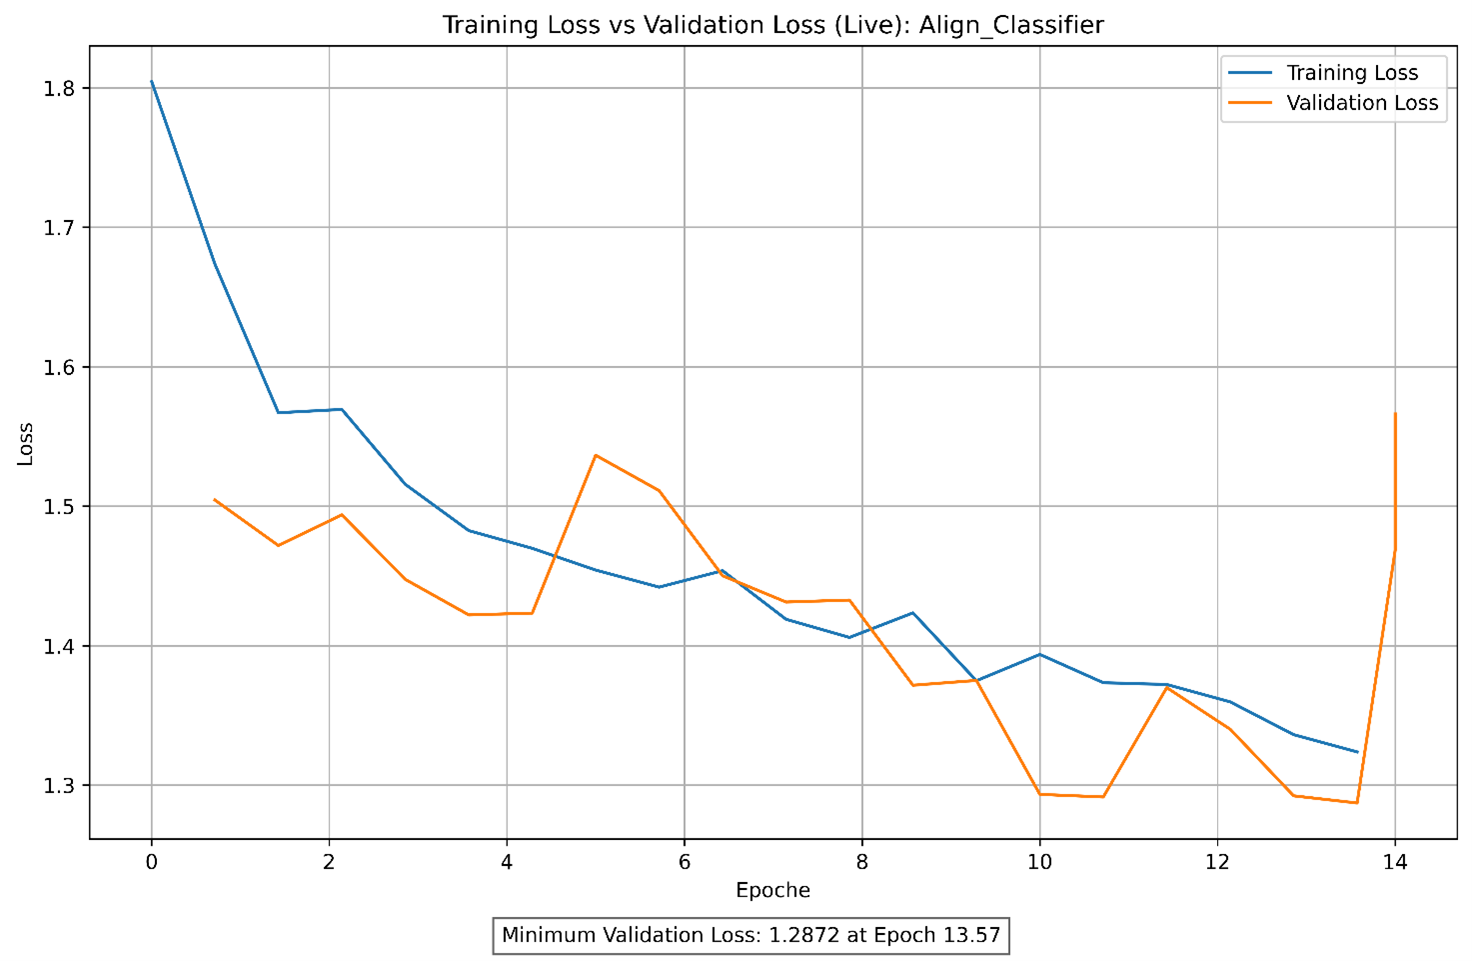
\includegraphics[width=0.8\textwidth]{img/bert/Immagine1.png}
\end{figure}

Osservando l’andamento della training loss, possiamo affermare che, si delinea una tendenza discendente, la quale suggerisce un apprendimento sano. Infatti, non si denota alcun asintoto orizzontalo che possano far sospettare la presenza di un minimo locale, che l’addestramento non riesce a superare.

L’addestramento prosegue sino alla soglia delle 14 epoche, questo perché, osservando l’andamento della validation loss, si può concludere che il modello migliora siano alla 13.57 epoca, oltre la quale la validation loss riscontra una crescita non trascurabile, il che può essere sintomo di over-fitting. Al termine del training viene prelevato il modello che ottiene un miglior risultato in fase di validation.

Si ricorda, che questa fase comprende solo l’ultimo livello del modello, per cui si ritiene difficile ottenere risultati migliori.

\begin{figure}[H]
    \centering
    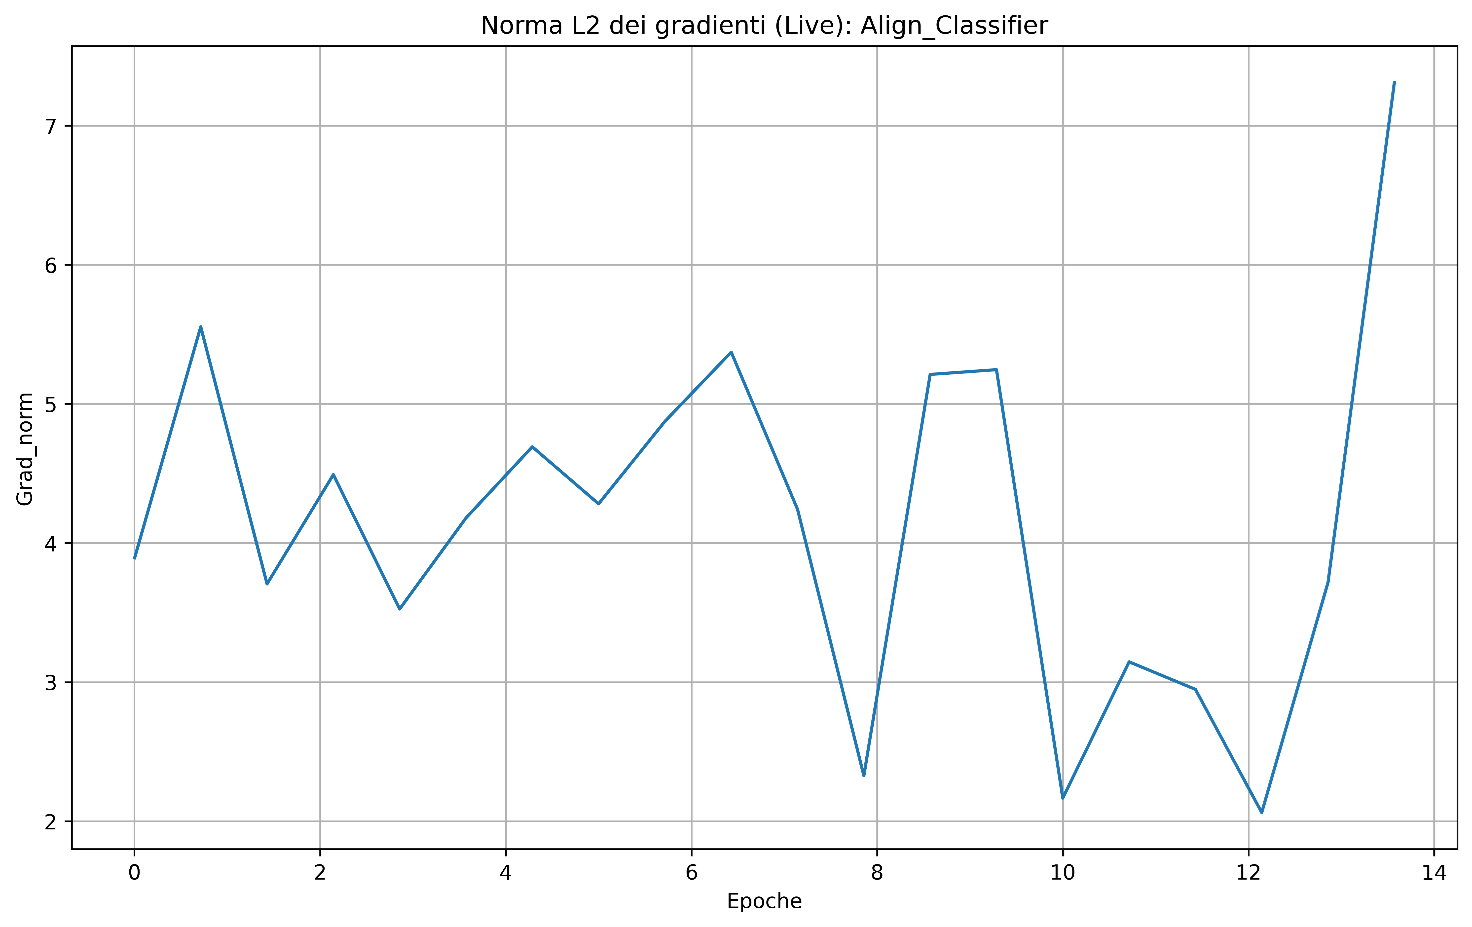
\includegraphics[width=0.8\textwidth]{img/bert/Immagine2.png}
\end{figure}

Per concludere l’analisi della fase di allineamento, si riporta anche l’andamento della norma L2 dei gradienti. Osservare questo parametro è essenziale per riconoscere fenomeni come il gradient vanishing e/o exploding. Nel nostro caso, la norma è stabile oscillando tra i valori 2 e 7.5, questo ci fa concludere che l’addestramento è stabile.

\subsubsection{Parametri Fine-tuning Completo}

\begin{table}[H]
    \centering
    \begin{tabular}{lc}
        \toprule
        Learning Rate & 2e-5  \\
        Weight Decay  & 0.001 \\
        Max Epochs    & 6     \\
        Batch Size    & 16    \\
        Fp16          & True  \\
        \bottomrule
    \end{tabular}
    \caption{Parametri per fine-tuning completo}
\end{table}

Durante questa fase di addestramento è stato adottato un approccio più prudente, caratterizzato da aggiornamenti dei parametri meno marcati e da una minore decadenza dei pesi, al fine di ridurre il rumore nel processo di ottimizzazione.

L’addestramento riportato di seguito rappresenta una procedura standard; sarebbe stato tuttavia possibile effettuare un processo più approfondito. Una volta definiti i parametri di training, si sarebbe potuto procedere utilizzando l’intero devset (training + validation), effettuando una suddivisione casuale tra training set e validation set. Successivamente, l’addestramento avrebbe potuto essere ripetuto più volte, calcolando media e varianza della training loss nel punto in cui la validation loss raggiunge il proprio valore minimo.

Infine, si sarebbe potuto eseguire un unico addestramento sull’intero devset, interrompendo il processo nel momento in cui la training loss avesse raggiunto il valore medio delle training loss osservate nei precedenti esperimenti.

\begin{figure}[H]
    \centering
    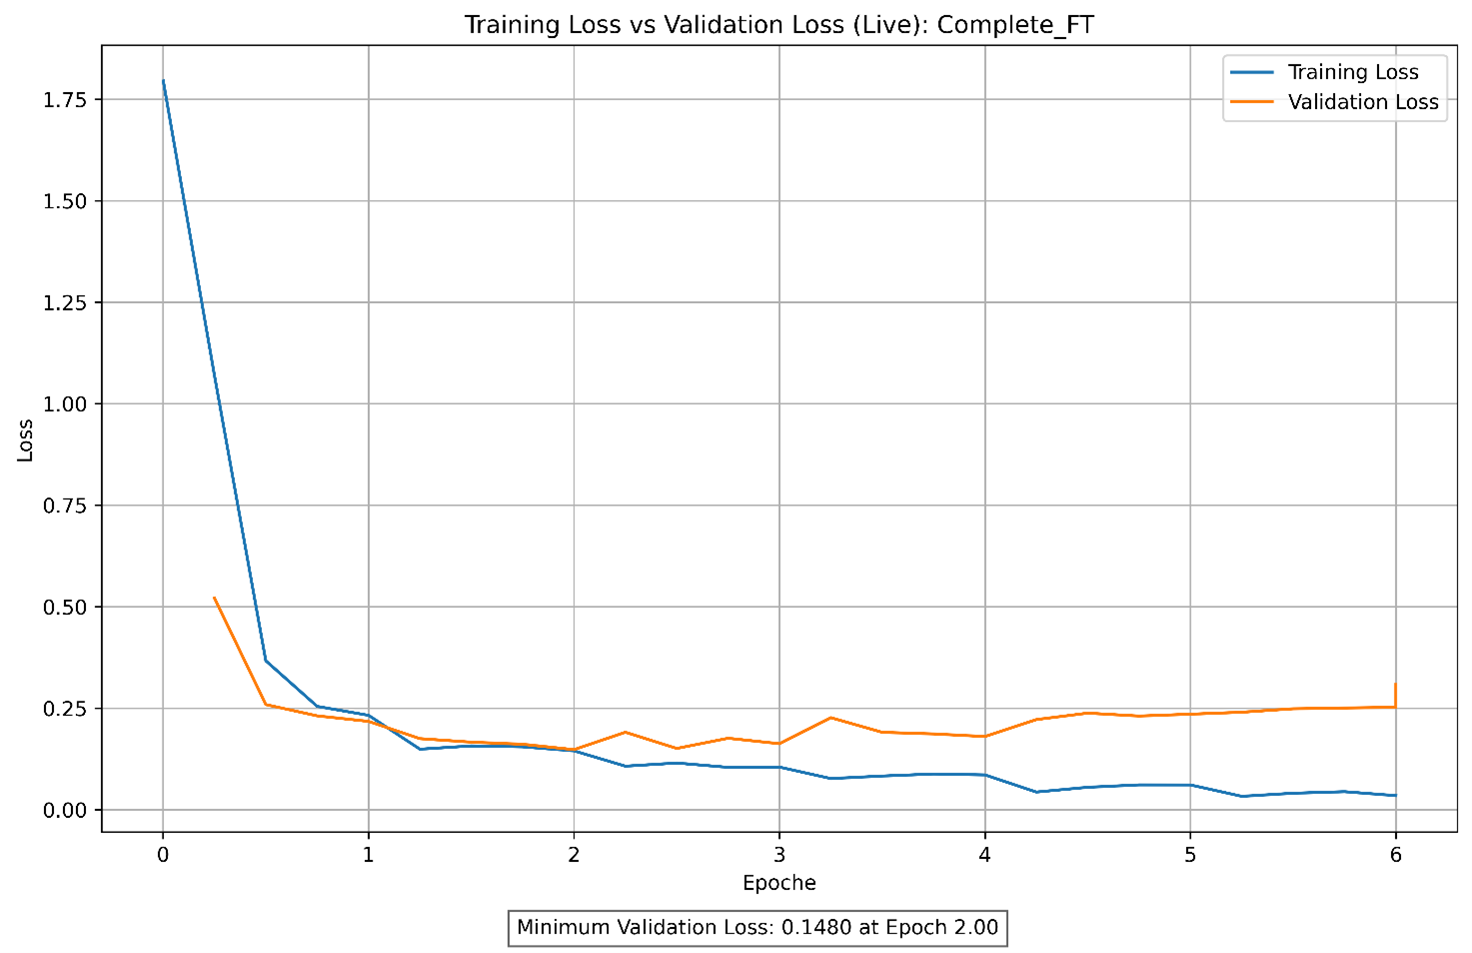
\includegraphics[width=0.8\textwidth]{img/bert/Immagine3.png}
\end{figure}

Si ripetono qui le stesse osservazioni fatte per la fase di allineamento. Tuttavia, a differenza della precedente fase, qui non si riscontra un’improvvisa risalita della validation loss, ma è più graduale; quindi, abbiamo proseguito l’addestramento per più tempo, così da essere ragionevolmente sicuri che questa non riprendesse più a scendere.

\begin{figure}[H]
    \centering
    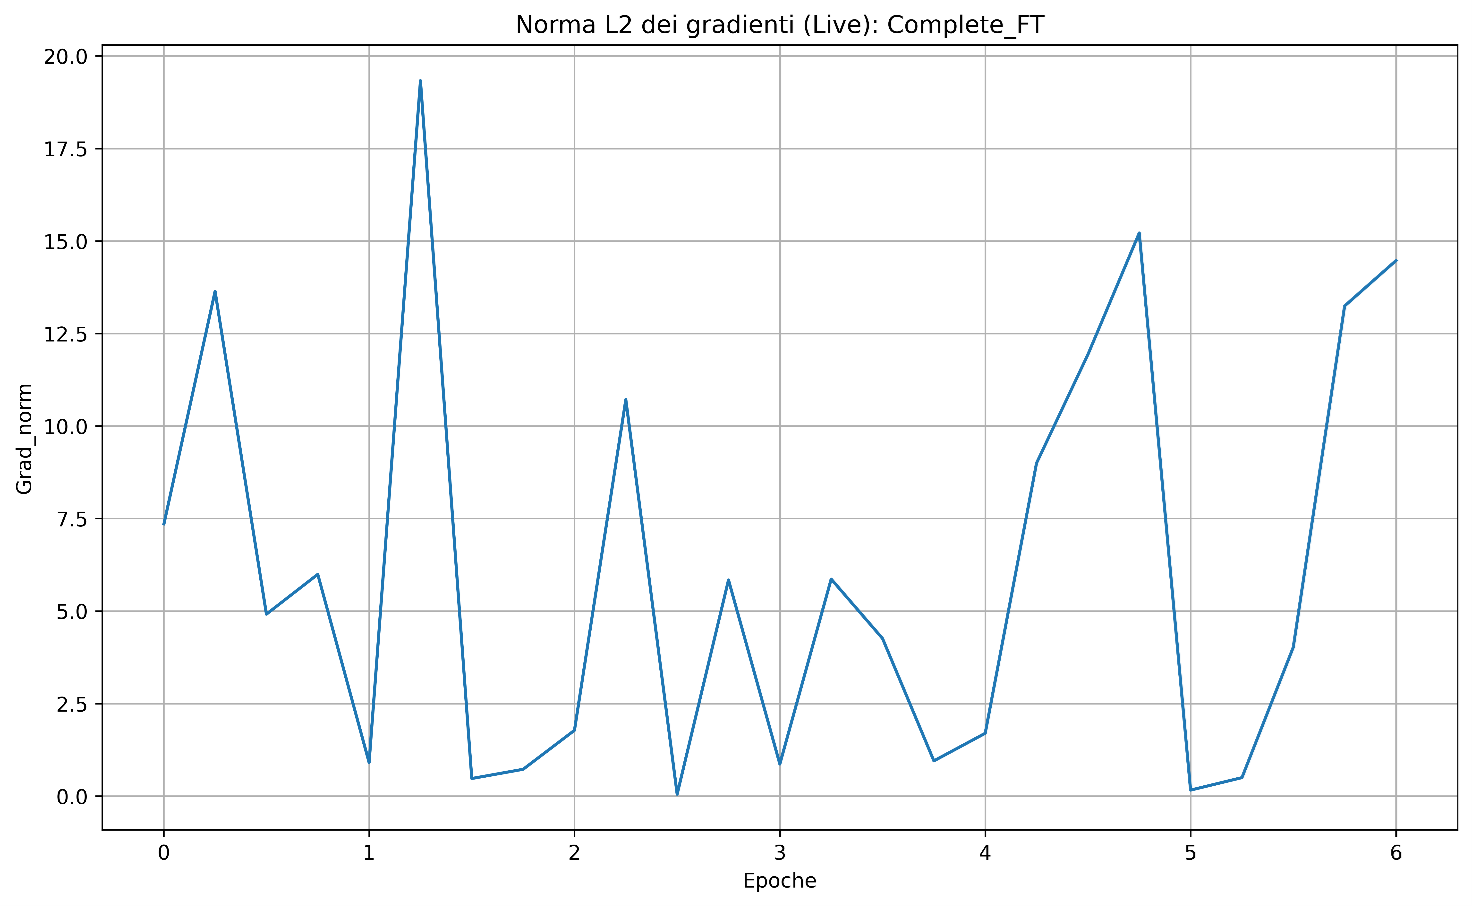
\includegraphics[width=0.8\textwidth]{img/bert/Immagine4.png}
\end{figure}

Per quanto riguarda lo studio della norma dei gradienti, in questo caso c’è una maggiore oscillazione, l’intervallo dei valori è maggiore. Tuttavia, si resta su valori sicuri e, inoltre, confrontandola con la training loss, si può riscontrare che gli spike isolati non hanno ripercussioni sull’addestramento.

\subsubsection{Risultati}

Di seguito sono riportate le performance dei migliori modelli, light fine-tuned e complete fine-tuned.

\subsubsection*{Performance inContext Learning}

Qui si valuta quanto il modello, allineato al task, riesca a performare utilizzando la tecnica di inContext learning applicata al test set. La valutazione è stata eseguita mediante 3 gradi di somministrazione:

\begin{enumerate}
    \item \textbf{One Shot}: i sample sono arricchiti dalla presenza di un esempio di applicazione del task.

    \item \textbf{Three Shot}: i sample sono arricchiti dalla presenza di tre esempi di applicazione del task.

    \item \textbf{Five Shot}: i sample sono arricchiti dalla presenza di cinque esempi di applicazione del task.
\end{enumerate}

Tuttavia, prima di presentare i risultati, è opportuno chiarire alcune definizioni relative alle principali metriche di valutazione utilizzate.

\begin{itemize}

\item \textbf{TP (True Positives)}: rappresentano i veri positivi, ovvero le predizioni corrette per una determinata classe.

\item \textbf{FP (False Positives)}: indicano i falsi positivi, ossia i casi in cui il modello predice la classe in esame quando in realtà l’osservazione appartiene a un’altra classe.

\item \textbf{FN (False Negatives)}: rappresentano i falsi negativi, ovvero i casi in cui il modello predice una classe diversa da quella effettiva, che invece corrisponde alla classe in esame.

\end{itemize}

A partire da tali quantità vengono definite alcune metriche di performance.

\begin{itemize}

\item \textbf{Precision}
\[
Precision = \frac{TP}{TP + FP}
\]

Questa metrica misura la proporzione di predizioni corrette tra tutte quelle assegnate alla classe considerata. È importante sottolineare che la precisione può assumere valore pari a 1 anche in presenza di una bassa accuratezza complessiva; ciò accade, ad esempio, quando il modello effettua una sola predizione per una determinata classe e questa risulta corretta.

\item \textbf{Recall}
\[
Recall = \frac{TP}{TP + FN}
\]

Questa metrica indica la capacità del modello di individuare correttamente tutte le istanze appartenenti alla classe considerata. Anche il recall può raggiungere valore pari a 1 pur in presenza di una bassa accuratezza globale, ad esempio nel caso in cui il modello tenda a predire sempre la stessa classe, sovrastimandone la presenza.

\end{itemize}

Per tali ragioni risulta opportuno considerare una metrica composita, quale l'\textbf{F1-score}, che consente di bilanciare precision e recall:

\[
F1 = 2 \times \frac{Precision \times Recall}{Precision + Recall}
\]

A supporto di quanto esposto, vengono di seguito riportate le \textbf{confusion matrix}, che permettono di rappresentare graficamente la distribuzione delle predizioni corrette ed errate del modello, fornendo una visione più immediata delle sue prestazioni.

\subsubsection*{One-Shot}

\begin{table}[H]
    \centering
    \begin{tabular}{cc}
        \toprule
        Metric & Value \\
        \midrule
        Accuracy & 0.4890 \\
        \bottomrule
    \end{tabular}
    \caption{Accuracy del modello in configurazione One-Shot}
\end{table}

\vspace{0.5cm}

\begin{table}[H]
    \centering
    \begin{tabular}{cccc}
        \toprule
        Class & Precision & Recall & F1     \\
        \midrule
        Sadness     & 0.4485    & 0.6970 & 0.5458 \\
        Joy     & 0.5234    & 0.8201 & 0.6390 \\
        Love     & 0.4285    & 0.0189 & 0.0361 \\
        Anger     & 0.0000    & 0.0000 & 0.0000 \\
        Fear     & 0.0000    & 0.0000 & 0.0000 \\
        Surprise     & 0.0000    & 0.0000 & 0.0000 \\
        \bottomrule
    \end{tabular}
    \caption{Metriche di precision, recall e F1 per classe in configurazione One-Shot}
\end{table}

\vspace{0.5cm}

\begin{figure}[H]
    \centering
    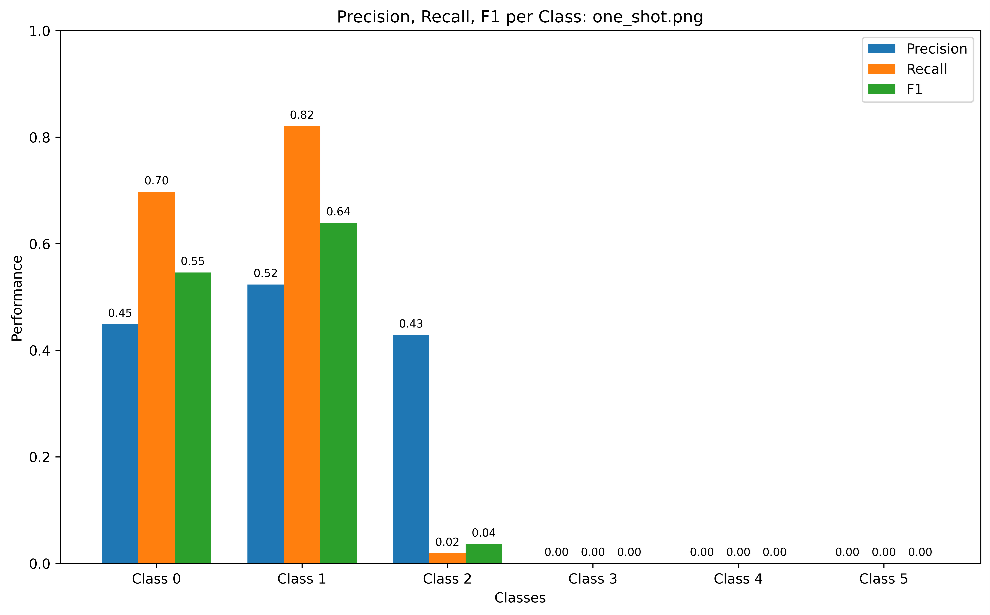
\includegraphics[width=0.6\textwidth]{img/bert/Immagine5.png}
    \caption{Rappresentazione grafica delle metriche in configurazione One-Shot}
\end{figure}

\vspace{0.5cm}

\begin{figure}[H]
    \centering
    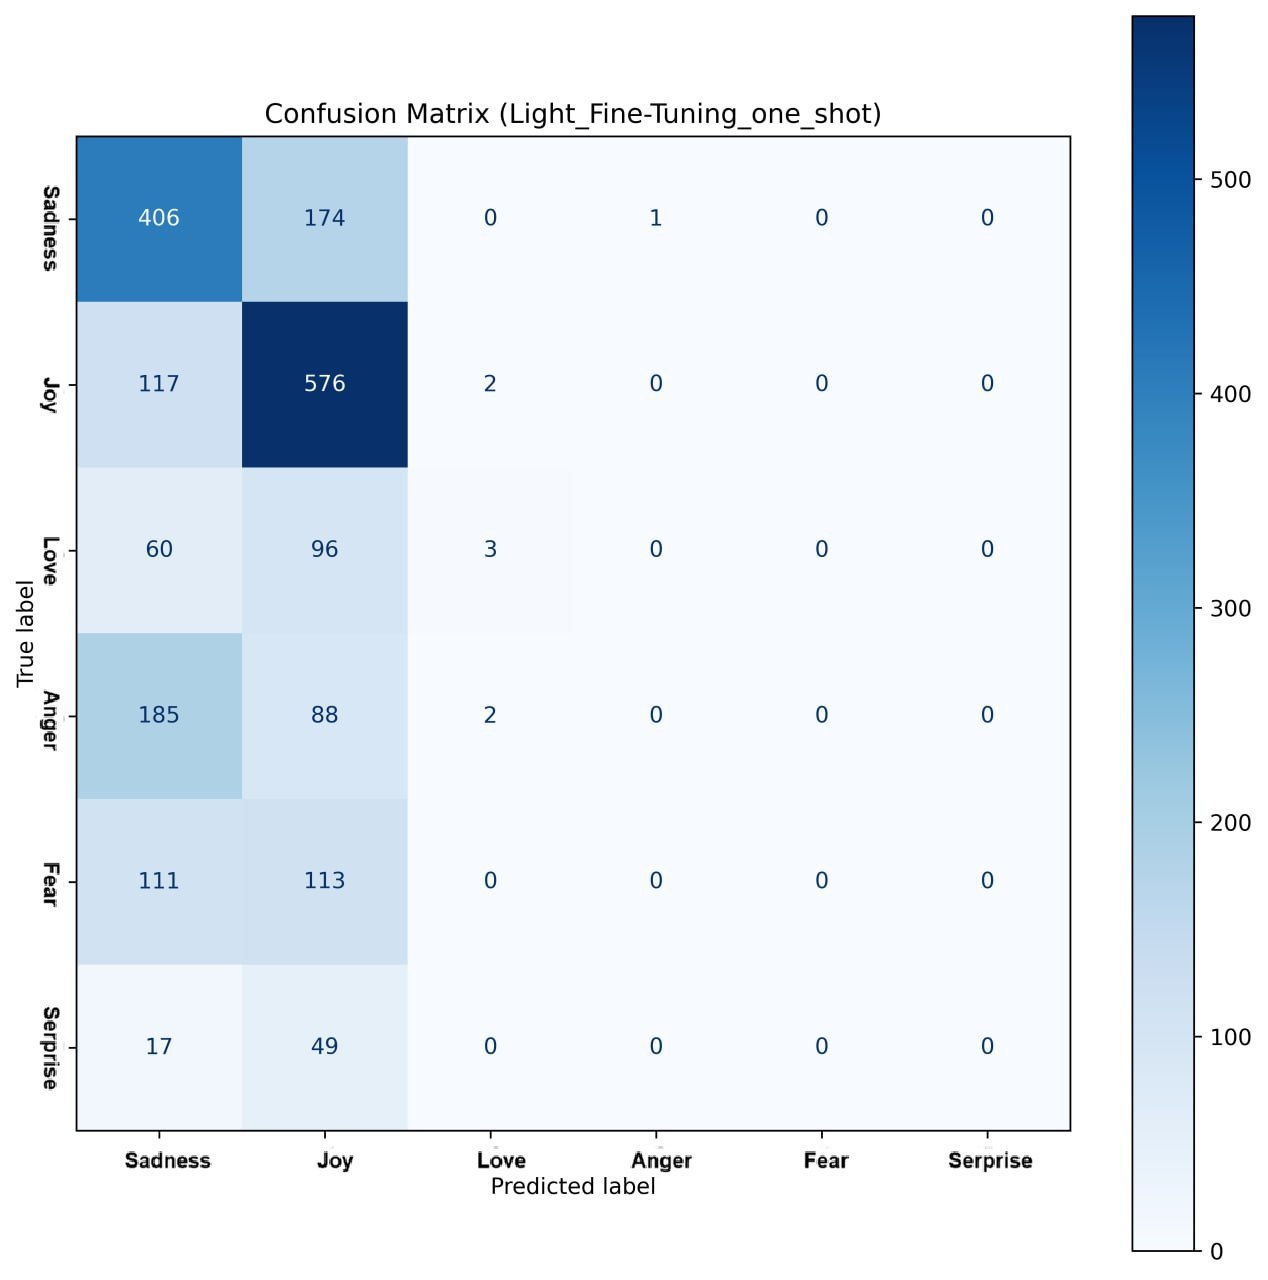
\includegraphics[width=0.6\textwidth]{img/bert/Immagine6.png}
    \caption{Confusion matrix del modello in configurazione One-Shot}
\end{figure}

\subsubsection*{Three-Shot}

\begin{table}[H]
    \centering
    \begin{tabular}{cc}
        \toprule
        Metric & Value \\
        \midrule
        Accuracy & 0.3870 \\
        \bottomrule
    \end{tabular}
    \caption{Accuracy del modello in configurazione Three-Shot}
\end{table}

\vspace{0.5cm}

\begin{table}[H]
    \centering
    \begin{tabular}{cccc}
        \toprule
        Class & Precision & Recall & F1     \\
        \midrule
        Sadness     & 0.5140    & 0.1583 & 0.2421 \\
        Joy     & 0.3752    & 0.9784 & 0.5425 \\
        Love     & 0.2222    & 0.0126 & 0.0238 \\
        Anger     & 0.0000    & 0.0000 & 0.0000 \\
        Fear     & 0.0000    & 0.0000 & 0.0000 \\
        Surprise     & 0.0000    & 0.0000 & 0.0000 \\
        \bottomrule
    \end{tabular}
    \caption{Metriche di precision, recall e F1 per classe in configurazione Three-Shot}
\end{table}

\vspace{0.5cm}

\begin{figure}[H]
    \centering
    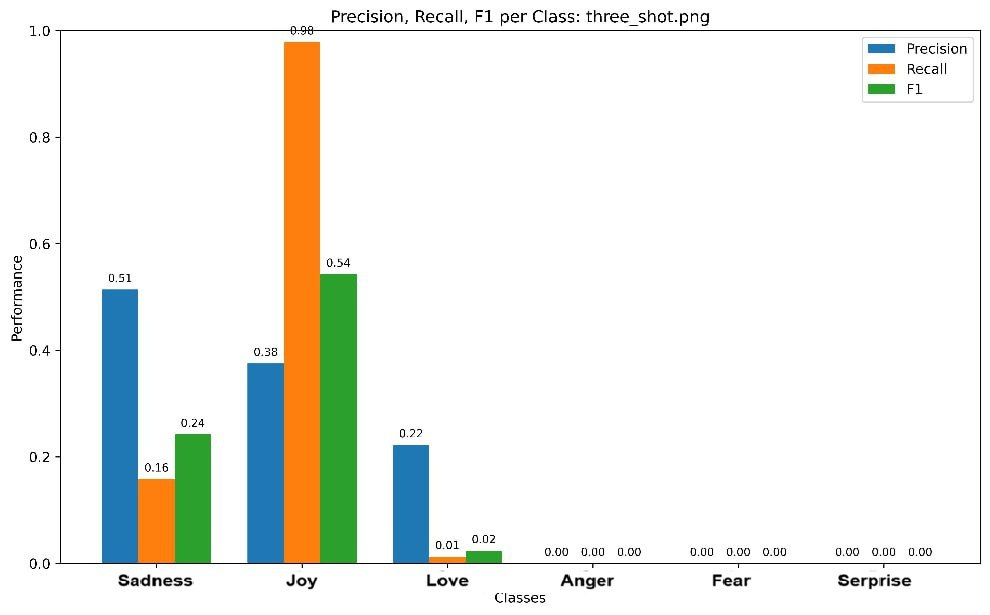
\includegraphics[width=0.6\textwidth]{img/bert/Immagine7.png}
    \caption{Rappresentazione grafica delle metriche in configurazione Three-Shot}
\end{figure}

\vspace{0.5cm}

\begin{figure}[H]
    \centering
    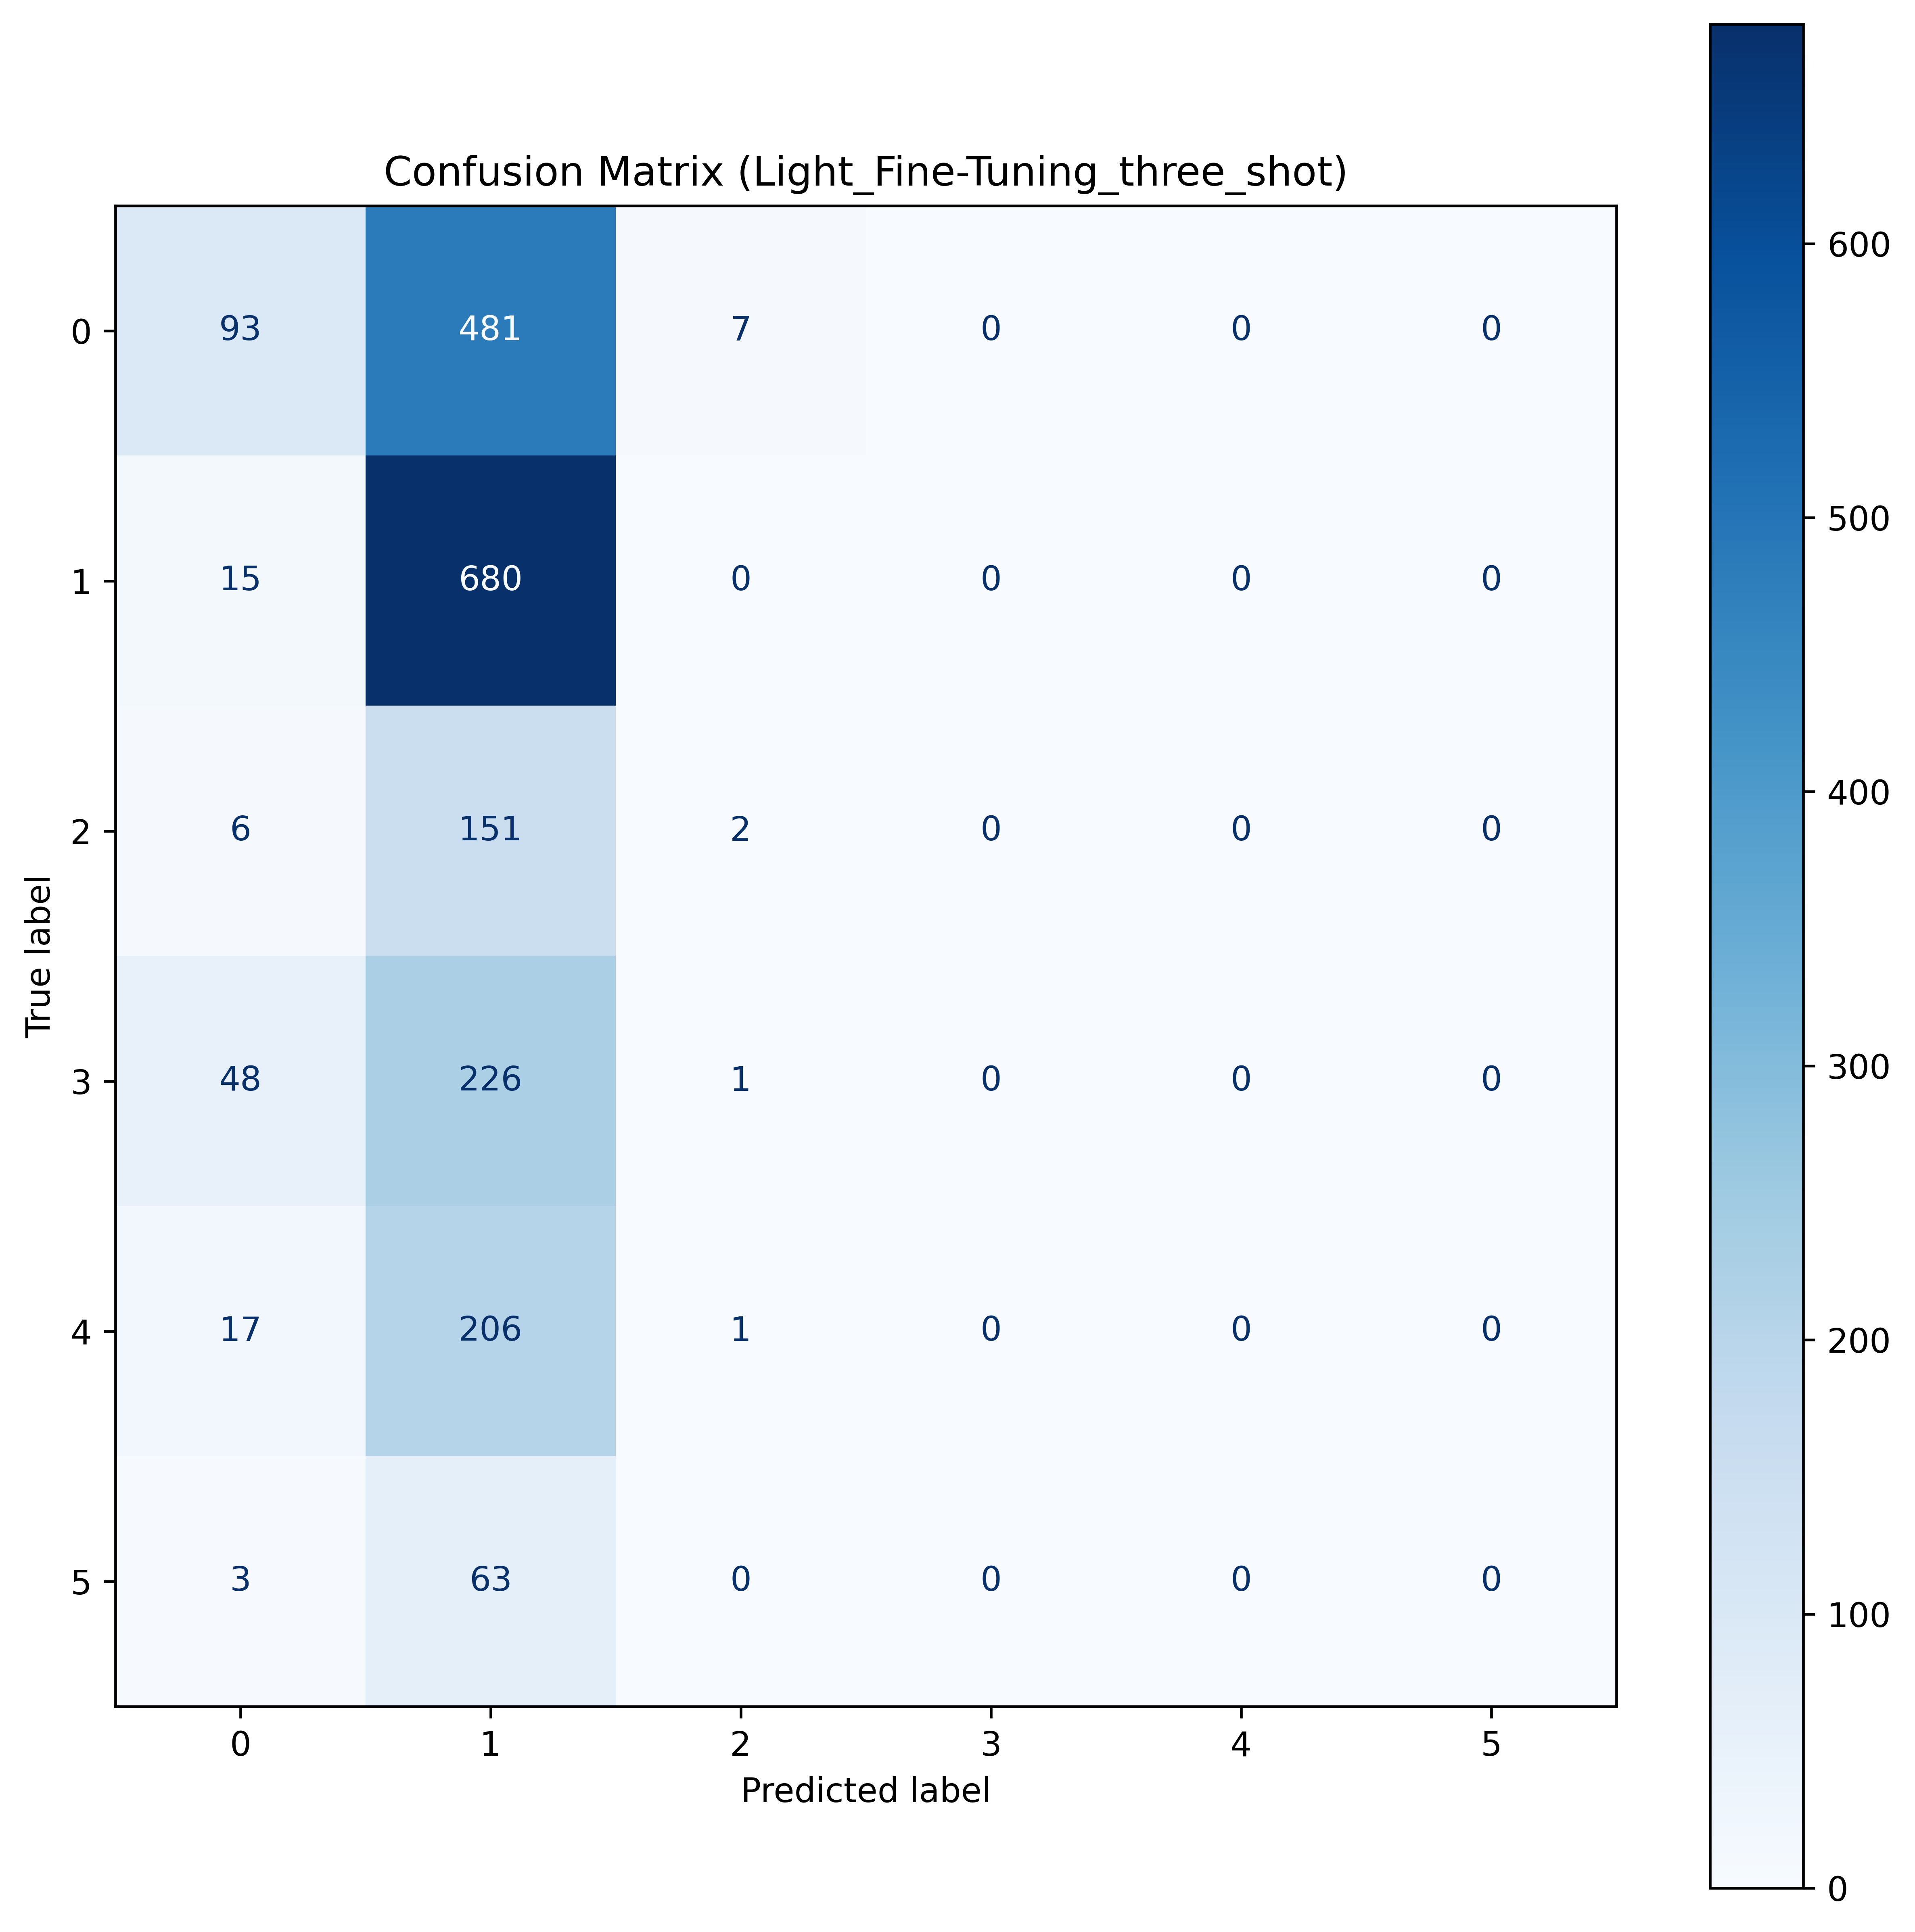
\includegraphics[width=0.6\textwidth]{img/bert/Immagine8.png}
    \caption{Confusion matrix del modello in configurazione Three-Shot}
\end{figure}

\subsubsection*{Five-Shot}

\begin{table}[H]
    \centering
    \begin{tabular}{cc}
        \toprule
        Metric & Value \\
        \midrule
        Accuracy & 0.4180 \\
        \bottomrule
    \end{tabular}
    \caption{Accuracy del modello in configurazione Five-Shot}
\end{table}

\vspace{0.5cm}

\begin{table}[H]
    \centering
    \begin{tabular}{cccc}
        \toprule
        Class & Precision & Recall & F1     \\
        \midrule
        Sadness     & 0.4673    & 0.3941 & 0.4276 \\
        Joy     & 0.4647    & 0.8158 & 0.5922 \\
        Love     & 0.1379    & 0.2516 & 0.1782 \\
        Anger     & 0.0000    & 0.0000 & 0.0000 \\
        Fear     & 0.0000    & 0.0000 & 0.0000 \\
        Surprise     & 0.0000    & 0.0000 & 0.0000 \\
        \bottomrule
    \end{tabular}
    \caption{Metriche di precision, recall e F1 per classe in configurazione Five-Shot}
\end{table}

\vspace{0.5cm}

\begin{figure}[H]
    \centering
    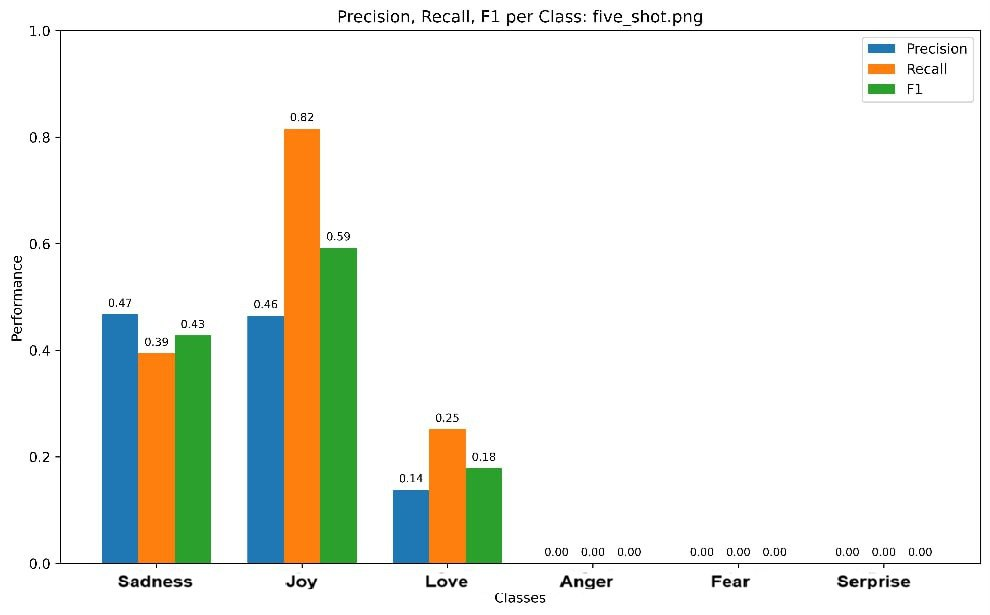
\includegraphics[width=0.6\textwidth]{img/bert/Immagine9.png}
    \caption{Rappresentazione grafica delle metriche in configurazione Five-Shot}
\end{figure}

\vspace{0.5cm}

\begin{figure}[H]
    \centering
    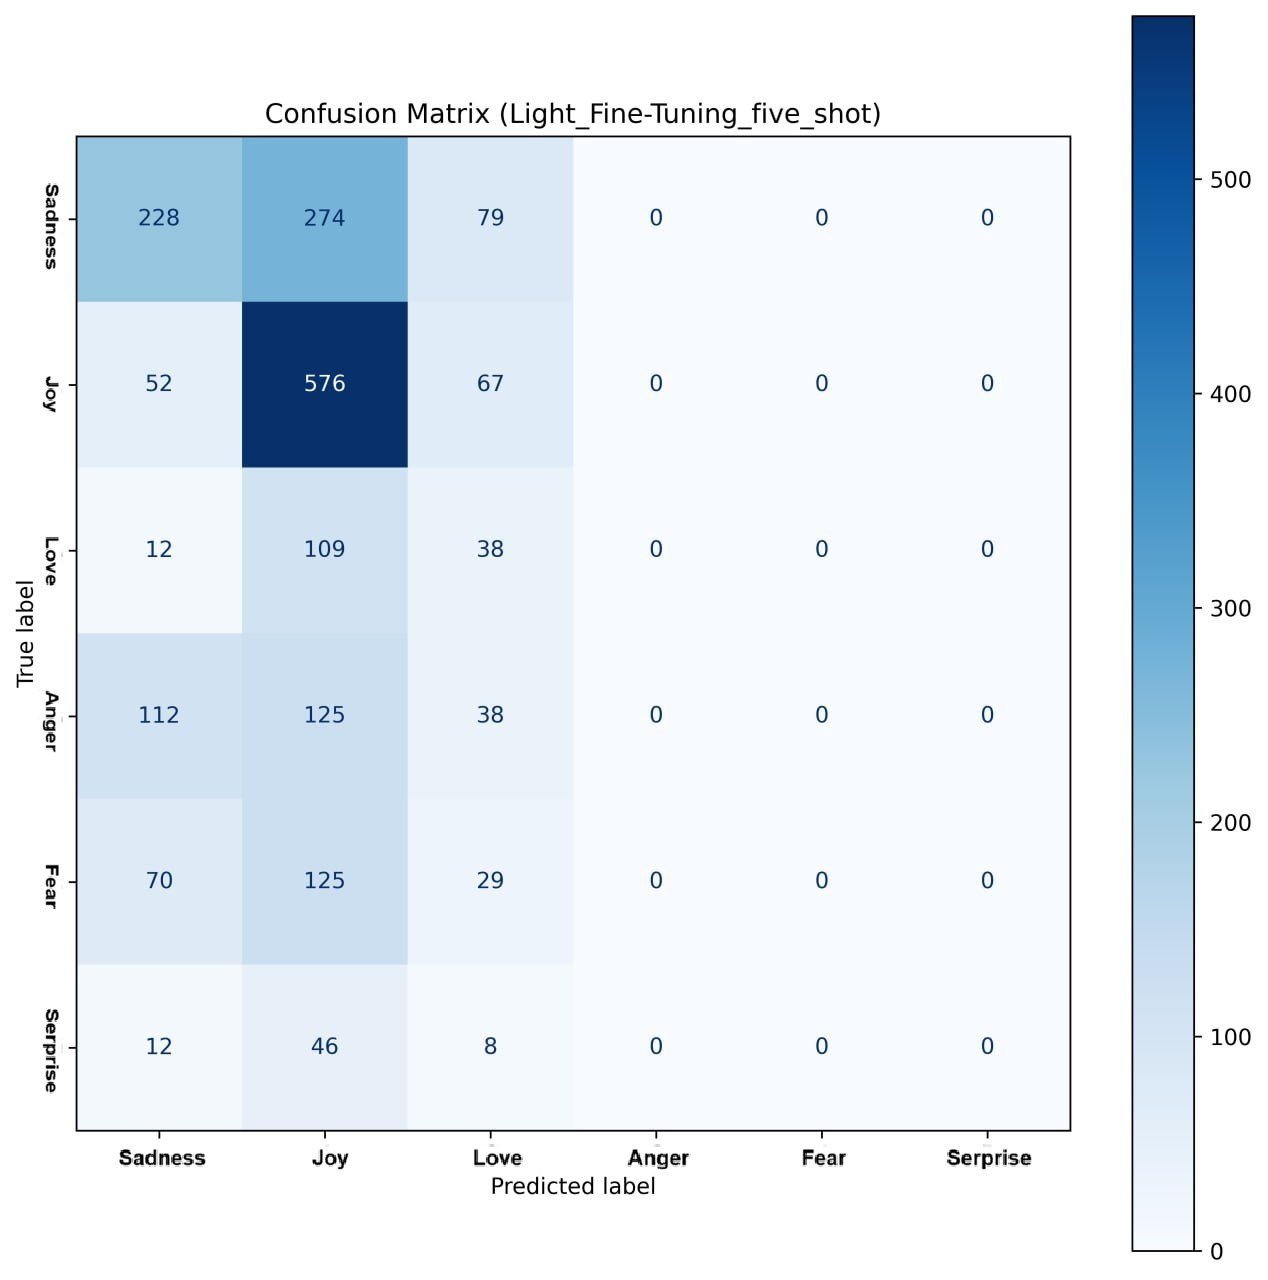
\includegraphics[width=0.6\textwidth]{img/bert/Immagine10.png}
    \caption{Confusion matrix del modello in configurazione Five-Shot}
\end{figure}

\subsubsection*{Confronto Performance In-Context}

In questa sezione si confrontano le performance dei vari gradi di inContext.

\begin{figure}[H]
    \centering
    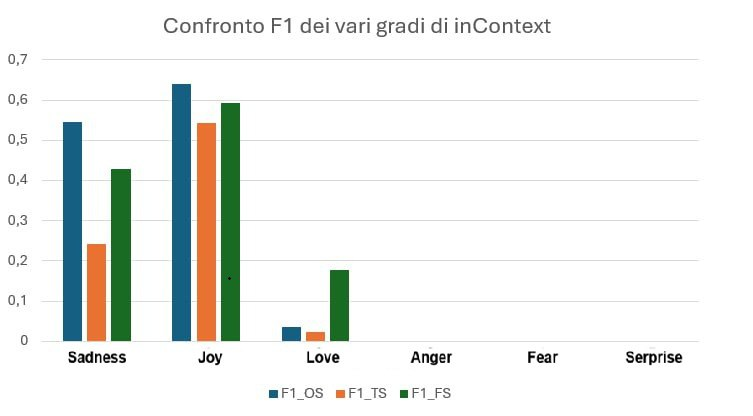
\includegraphics[width=0.8\textwidth]{img/bert/Immagine11.png}
\end{figure}

Osservando le metriche a confronto, si può riscontrare l’assenza di nette variazioni nelle prestazioni. Incrementando il numero di esempi in input per il modello, questo non incrementa le sue capacità. Questo conferma la natura di abilità emergente, dei modelli decoder di grandi dimensioni, dell’abilità esercitata.

\subsubsection*{Performance Fine-tuning Completo}

In questa sezione si espongono le performance del modello sul test set senza l’applicazione della tecnica di inContext.

\begin{table}[H]
    \centering
    \begin{tabular}{cc}
        \toprule
        Metric & Value \\
        \midrule
        Accuracy & 0.9300 \\
        \bottomrule
    \end{tabular}
    \caption{Accuracy del modello dopo Fine-tuning Completo}
\end{table}

\vspace{0.5cm}

\begin{table}[H]
    \centering
    \begin{tabular}{cccc}
        \toprule
        Class & Precision & Recall & F1     \\
        \midrule
        Sadness     & 0.9641    & 0.9707 & 0.9674 \\
        Joy     & 0.9602    & 0.9381 & 0.9490 \\
        Love     & 0.8095    & 0.8553 & 0.8318 \\
        Anger     & 0.9200    & 0.9200 & 0.9200 \\
        Fear     & 0.8707    & 0.9018 & 0.8860 \\
        Surprise     & 0.7377    & 0.6818 & 0.7087 \\
        \bottomrule
    \end{tabular}
    \caption{Metriche di precision, recall e F1 per classe dopo Fine-tuning Completo}
\end{table}

\vspace{0.5cm}

\begin{figure}[H]
    \centering
    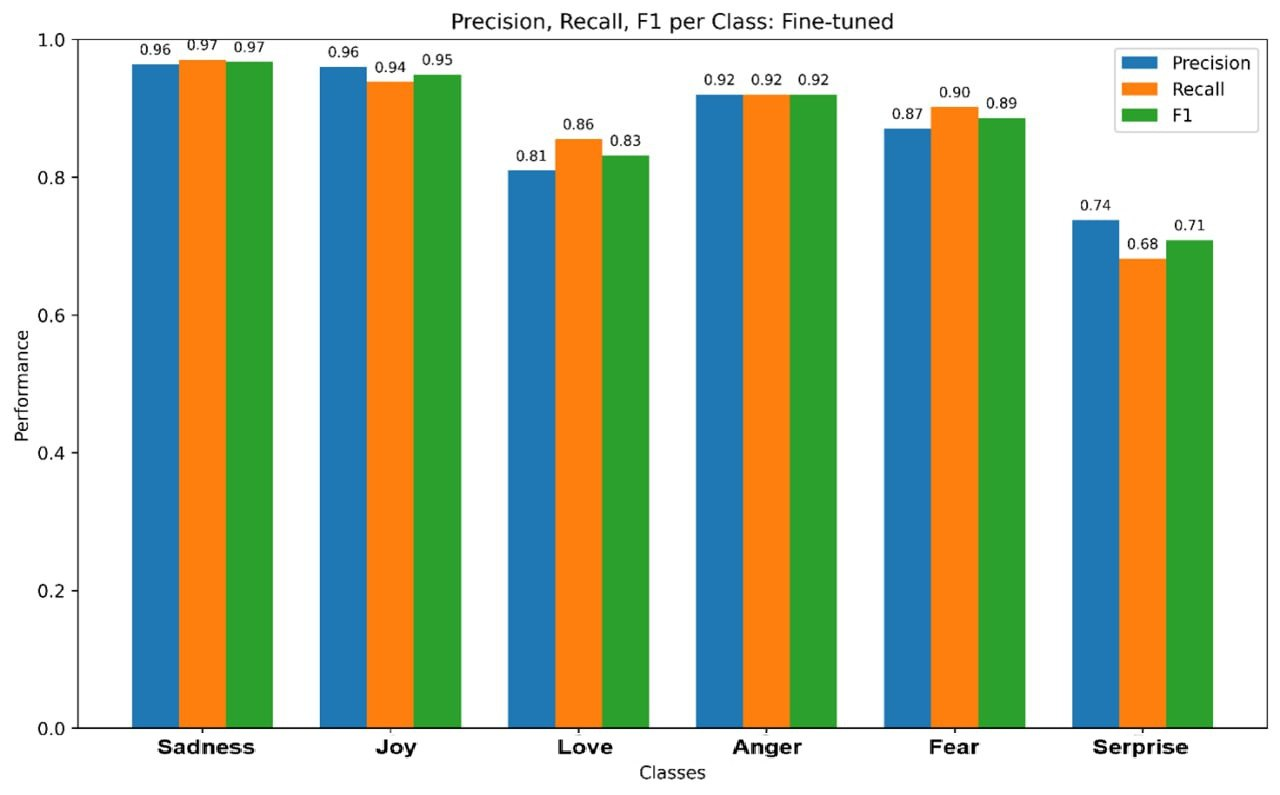
\includegraphics[width=0.8\textwidth]{img/bert/Immagine12.png}
    \caption{Rappresentazione grafica delle metriche dopo Fine-tuning Completo}
\end{figure}

Si osserva un netto incremento delle prestazioni del modello. Tuttavia, si sottolinea che queste sono direttamente proporzionali alle dimensioni delle partizioni dei datasets. Il modello ottiene risultati migliori in presenza delle classi predominanti nei dati (Classe Sadness e Joy), al contrario, classi più rare (Classe Love e Surprise) mettono in difficoltà il modello. In conclusione, le prestazioni del modello riflettono la natura sbilanciata dei datasets.

\vspace{0.5cm}

\begin{figure}[H]
    \centering
    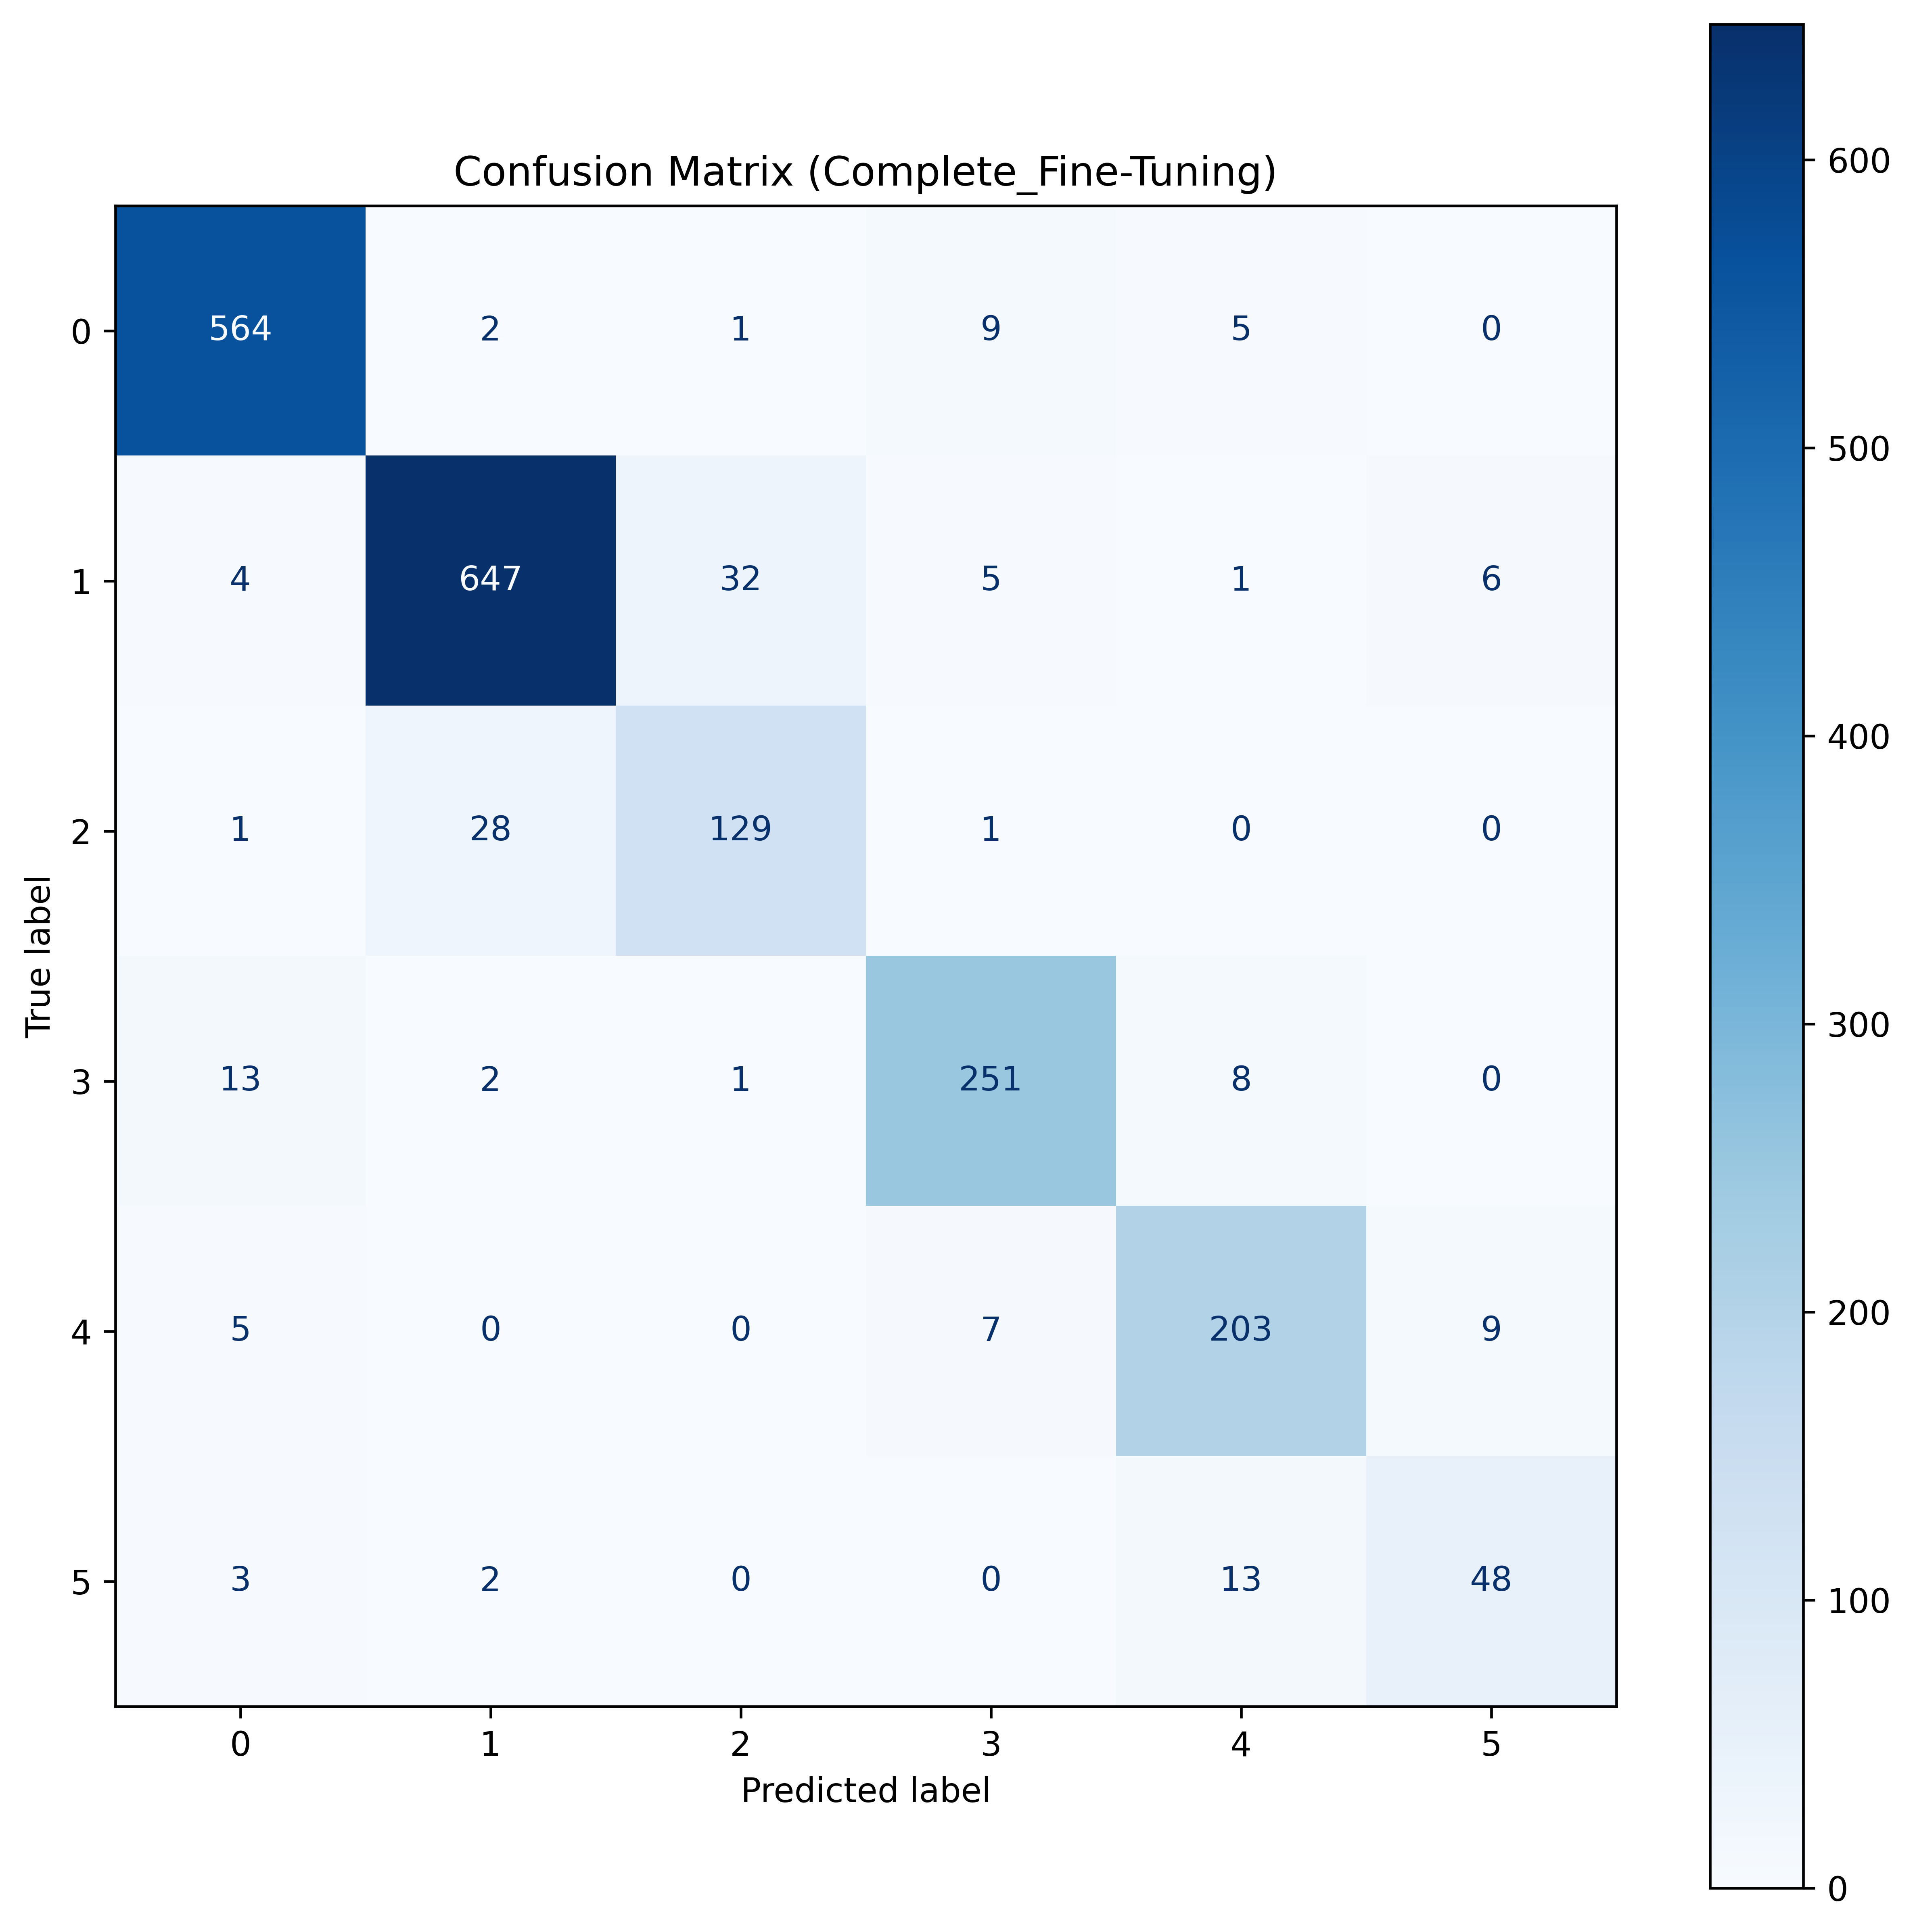
\includegraphics[width=0.8\textwidth]{img/bert/Immagine13.png}
    \caption{Confusion matrix del modello dopo Fine-tuning Completo}
\end{figure}


\subsection{roberta-base}
\subsubsection{Modello}
\textbf{RoBERTa} sta  per \textbf{R}obustly \textbf{o}ptimized \textbf{BERT} \textbf{a}pproach ed è un modello pre-addestrato con l’obiettivo di Masked Language Modeling (MLM). Data in input una frase, il modello maschera casualmente il 15\% delle parole, elaborando l’intera frase mascherata e deve predire le parole che sono state oscurate. Il modello in questione (RoBERTa-base) si presenta con un numero di parametri allenabili pari a $124,650,246$.

\subsubsection{Dimostrazione e Tecnologie}
L'analisi del modello è stata eseguita utilizzando le seguenti tecnologie:
\begin{itemize}
    \item \textbf{Environment:} Google Colab (Python 3) con runtime T4 GPU.
    \item \textbf{Librerie:}
          \begin{itemize}
              \item \texttt{transformers} libreria di HuggingFace per la gestione dei modelli
              \item \texttt{datasets} e \texttt{evaluate} per la gestione dei dati e delle metriche.
              \item \texttt{scikit-learn} per il calcolo delle matrici di confusione.
              \item \texttt{peft} libreria di HuggingFace per l'implementazione di LoRA.
              \item \texttt{numpy} e \texttt{matplotlib} per l'analisi dei dati.
              \item \texttt{google} già presente su Colab per la connessione a Google Drive.
          \end{itemize}
\end{itemize}
Per poter riprodurre i risultati è necessario rieseguire tutte le celle del notebook. A causa dei limiti di utilizzo della T4 GPU di Google Colab, l'esecuzione potrebbe essere interrotta prima del completamento. Per questo motivo è stato collegato Google Drive per il salvataggio dei modelli.

\subsubsection{Risultati}
Dopo aver testato differenti tecniche, l'esito migliore è stato raggiunto con la strategia di \textbf{Full Fine-Tuning} che ha ottenuto i seguenti risultati sul Validation Set:
\begin{itemize}
    \item \textbf{Accuracy:} 94.15\%
    \item \textbf{Macro F1-Score:} 91.86\%
    \item \textbf{Training Time:} $\sim$10:30 (5/10 epoche - Early stopping dopo 2 epoche).
\end{itemize}

La configurazione utilizza un Learning Rate di $2e^{-5}$, un Batch Size di $16$, un Weight Decay di $0.01$ e un indice di Warmup Steps di $0.1$.

\subsubsection{Ablation Study: Analisi delle Configurazioni}
Lo studio di Ablation è stato svolto in quattro fasi dell'analisi con lo scopo di determinare la configurazione di iperparametri di maggior efficienza:
\begin{itemize}
    \item \textbf{A. Transfer Learning:} i pesi del modello base vengono "congelati", impedendo qualsiasi aggiornamento durante il training. Solo la classification head viene allenata, adattando il modello RoBERTa alle classi del task.
    \item \textbf{B. Full Fine-Tuning:} tutti i pesi del modello base vengono aggiornati durante il training, consentendo al modello di specializzarsi completamente sul task. Questo approccio peò richiede risorse computazionali significative.
    \item \textbf{C. LoRA (Low Rank Adaptation):} anzichè aggiornare direttamente i pesi del modello, si introducono due matrici di rango ridotto. Solo queste matrici vengono poi addestrate, riducendo drasticamente il numero di parametri.
    \item \textbf{D. In-Context Learning (ICL):} il modello viene utilizzato senza alcun aggiornamento dei pesi. Nel caso few-shot, alcuni esempi etichettati vengono forniti direttamente nel prompt guidando la predizione.
\end{itemize}

\subsubsection*{A. Transfer Learning (Allineamento solo della Classification Head)}
I parametri del corpo del modello base sono stati "congelati" ad eccezione della testa di classificazione ($595,206$ parametri allenabili) ed è stata eseguita una ricerca completa comparando sei configurazioni differenti tra tre valori di Learning Rate $\in \{1e^{-3}, 1e^{-4}, 1e^{-5}\}$ e due dimensioni di Batch Size $\in \{16, 32\}$.
Analizzando i risultati della ricerca risulta che, con l'utilizzo di un valore di learning rate maggiore ($1e^{-3}$) si ottiene un addestramento della testa di classificazione più efficiente rispetto a valori inferiori:
\begin{itemize}
    \item $1e^{-3}$ produce le performance migliori in entrambe le configurazioni di batch size, mentre valori inferiori degradano progressivamente.
    \item In particolare, $1e^{-5}$ produce risultati identici indipendentemente dalla batch size (34.75\% accuracy, 8.60\% F1), suggerendo che un learning rate eccessivamente basso impedisce qualsiasi aggiornamento significativo dei pesi della testa di classificazione.
\end{itemize}
I risultati migliori raggiunti risultano avere un valore di accuracy del $57.95\%$ e un valore di F1-Score del $32.50\%$, non abbastanza efficienti per il task di text emotion classification rispetto ad altre strategie analizzate in seguito.

\begin{table}[H]
    \centering
    \begin{tabular}{|c|c|c|c|}
        \hline
        \textbf{Learning Rate} & \textbf{Batch Size} & \textbf{Accuracy} & \textbf{F1-Score} \\
        \hline
        $1e^{-3}$              & 16                  & \textbf{57.95\%}  & \textbf{32.50\%}  \\
        $1e^{-3}$              & 32                  & 56.80\%           & 30.66\%           \\
        $1e^{-4}$              & 16                  & 51.45\%           & 20.68\%           \\
        $1e^{-4}$              & 32                  & 49.65\%           & 19.88\%           \\
        $1e^{-5}$              & 16                  & 34.75\%           & 08.60\%           \\
        $1e^{-5}$              & 32                  & 34.75\%           & 08.60\%           \\
        \hline
    \end{tabular}
    \caption{Risultati delle configurazioni per l'allineamento della testa di classificazione}
\end{table}

\subsubsection*{B. Full Fine-Tuning}
La seconda tecnica applicata è stata il Full Fine-Tuning. In questo caso è stato allenato il $100\%$ dei parametri ($124,650,246$) ed è stata eseguita una ricerca completa comparando sei configurazioni differenti tra tre valori di Learning Rate $\in \{1e^{-5}, 2e^{-5}, 3e^{-5}\}$ e due dimensioni di Batch Size $\in \{16, 32\}$ come citato nel paper di riferimento presentato da Yinhan Liu et al. (2019) \cite{yinhan-liu-etal-2019-roberta}.
La configurazione che ha ottenuto i risultati migliori utilizza un valore di Learning Rate di $2e^{-5}$ e una dimensione di Batch Size di $16$, raggiungendo un valore di accuracy del $93.10\%$ e un valore di F1 macro del $89.26\%$. In generale, l'utilizzo di un Learning Rate nell'intervallo $\{1e^{-5}, 2e^{-5}, 3e^{-5}\}$ produce risultati stabili e consistenti, con un valore di accuracy sempre superiore al $92\%$ e un valore di F1-macro maggiore del $88\%$, confermando la robustezza del Full Fine-Tuning rispetto alla scelta degli iperparametri in questo intervallo.

\begin{table}[H]
    \centering
    \begin{tabular}{|c|c|c|c|}
        \hline
        \textbf{Learning Rate} & \textbf{Batch Size} & \textbf{Accuracy} & \textbf{F1-Score} \\
        \hline
        $2e^{-5}$              & 16                  & \textbf{93.10\%}  & \textbf{89.26\%}  \\
        $1e^{-5}$              & 32                  & 92.60\%           & 88.80\%           \\
        $2e^{-5}$              & 32                  & 92.75\%           & 88.40\%           \\
        $3e^{-5}$              & 32                  & 92.90\%           & 88.28\%           \\
        $3e^{-5}$              & 16                  & 92.30\%           & 88.16\%           \\
        $1e^{-5}$              & 16                  & 92.50\%           & 88.03\%           \\
        \hline
    \end{tabular}
    \caption{Risultati delle configurazioni di Full Fine-Tuning}
\end{table}

\subsubsection*{C. LoRA}
La caratteristica fondamentale di LoRA è il numero di parametri addestrabili. Grazie a questa strategia anziche allenare il $100\%$ dei perametri, ne sono stati allenati solamente $1,479,942$ per le configurazioni con un rango di $16$ e $2,364,678$ per le configurazioni con rango pari a $32$, un utilizzo pari al $1.8\%$ dei parametri totali del modello.
Per individuare la configurazione LoRA ottimale, è stata condotta una ricerca su 12 combinazioni di iperparametri tra Rango ($16, 32$), Learning Rate ($5e^{-5}$, $1e^{-4}$, $5e^{-4}$) e Batch Size ($8, 16$).
La configurazione migliore ($r=32$, LR $5e^{-4}$, BS $16$) raggiunge un'accuracy del 92.65\% e un F1-score macro dell'88.46\%. In generale, $r=32$ ottiene risultati leggermente superiori a $r=16$ a parità di altri iperparametri.
Il learning rate risulta essere l'iperparametro di maggior impatto. Valori bassi come $5e^{-5}$ producono performance inferiori, mentre valori di LR di $1e^{-4}$ e $5e^{-4}$ garantiscono risultati migliori.
Si puo osservare, però, un caso di \textit{training collapse} nella configurazione ($r=32$, LR $5e^{-4}$, BS $8$), che crolla ad un accuracy del 34.75\% e un F1 dell'8.60\%. Osservando la configurazione identica con BS $16$ è possibile notare che non mostra questo problema, suggerendo che batch size ridotte possano amplificare l'instabilità del gradiente se combinati a valori di learning rate elevati e ranghi alti.

\begin{table}[H]
    \centering
    \small
    \begin{tabular}{|c|c|c|c|c|l|}
        \hline
        \textbf{Rank} & \textbf{LR} & \textbf{BS} & \textbf{Accuracy} & \textbf{F1-Score} \\
        \hline
        32            & $1e^{-4}$   & 8           & 92.45\%           & 88.61\%           \\
        32            & $5e^{-4}$   & 16          & \textbf{92.65\%}  & \textbf{88.46\%}  \\
        16            & $5e^{-4}$   & 16          & 92.45\%           & 88.46\%           \\
        16            & $5e^{-4}$   & 8           & 92.45\%           & 88.36\%           \\
        32            & $1e^{-4}$   & 16          & 92.50\%           & 88.24\%           \\
        16            & $1e^{-4}$   & 8           & 92.20\%           & 88.08\%           \\
        16            & $1e^{-4}$   & 16          & 91.25\%           & 86.87\%           \\
        32            & $5e^{-5}$   & 8           & 91.00\%           & 86.60\%           \\
        16            & $5e^{-5}$   & 8           & 90.60\%           & 86.42\%           \\
        32            & $5e^{-5}$   & 16          & 90.55\%           & 86.41\%           \\
        16            & $5e^{-5}$   & 16          & 88.85\%           & 84.15\%           \\
        32            & $5e^{-4}$   & 8           & 34.75\%           & 08.60\%           \\
        \hline
    \end{tabular}
    \caption{Risultati delle configurazioni LoRA}
\end{table}

\subsubsection*{D. In-Context Learning (Zero-Shot e Few-Shots)}
È opportuno sottolineare che RoBERTa è un modello encoder-only addestrato con un obiettivo di Masked Language Modeling (MLM); a differenza dei modelli decoder generativi, non è stato progettato per l'ICL, e di conseguenza i risultati vanno interpretati tenendo conto di questa considerazione.
Con la configurazione zero-shot, il modello raggiunge la performance migliore, con un'accuracy del 51.15\% e un F1-score macro del 26.73\%. Il divario tra accuracy e F1-score macro suggerisce un comportamento sbilanciato del modello, che tende a predire correttamente le classi più frequenti ignorando quelle minoritarie. Con l'aggiunta di esempi nel contesto le performance peggiorano: la configurazione 1-shot registra il calo più marcato (accuracy 43.53\%, F1 21.22\%), mentre 3-shot e 5-shot mostrano un lieve recupero, pur rimanendo al di sotto della configurazione zero-shot. Tale andamento è prevedibile data l'architettura di RoBERTa-base.
Il modello non è stato ottimizzato per il condizionamento del contesto come fa l'ICL e, di conseguenza, gli esempi aggiuntivi possono interferire con il pattern del prompt atteso dal MLM. È opportuno precisare che, in tutte le configurazioni, non sono stati registrati troncamenti del token \texttt{<mask>}, escludendo quindi risultati legati alla lunghezza del contesto.

\begin{table}[H]
    \centering
    \begin{tabular}{|c|c|c|}
        \hline
        \textbf{Shots} & \textbf{Accuracy} & \textbf{F1-Score} \\
        \hline
        0              & \textbf{51.15\%}  & \textbf{26.73\% } \\
        1              & 43.53\%           & 21.22\%           \\
        3              & 45.77\%           & 22.76\%           \\
        5              & 46.35\%           & 23.70\%           \\
        \hline
    \end{tabular}
    \caption{Risultati dell'In-Context Learning Zero-Shot e Few-Shots}
\end{table}

\subsubsection{Analisi degli errori}
L'analisi degli errori, eseguita con il modello sul quale è stata applicata la strategia di Full Fine-Tuning con risultati migliori, mostra che il maggior numero di errori di classificazione si concentra su determinate classi di emozioni:


\begin{enumerate}
    \item \textbf{Love} e \textbf{joy:} La classe \textit{joy} risulta tra le più riconosciute dal modello. La classe \textit{love}, invece, registra la performance peggiore con il 19\% degli esempi classificati erroneamente come \textit{joy}. Questo errore è semanticamente motivato: testi che esprimono amore condividono spesso un tono positivo e lessico affine a quelli di gioia, rendendo il confine tra le due classi ambiguo. Di seguito vengono mostrati alcuni esempi di errore:
          \begin{itemize}
              \item \textbf{Testo:} \textit{`i feel the need to work on caring`} $\rightarrow$ \textbf{True:} love,
                    \textbf{Predicted:} joy
              \item \textbf{Testo:} \textit{`i was not feeling up to it yet i blamed my fiances deployment for bringing me down`} $\rightarrow$ \textbf{True:} love,
                    \textbf{Predicted:} joy
              \item \textbf{Testo:} \textit{`i feel unimportant and small here lately`} $\rightarrow$ \textbf{True:} love,
                    \textbf{Predicted:} joy
          \end{itemize}
          Su un totale di 2000 esempi, la classe \textit{love} viene confusa con \textit{joy} 30 volte.

    \item \textbf{Surprise} e \textbf{Fear:} Anche in questo caso, la classe \textit{surprise} risulta tra le piu riconosciute, mentre \textit{fear} è la classe che presenta il maggior numero di errori. Il 12\% degli esempi di \textit{fear} viene classificato come \textit{surprise}, e il restante 8\% si distribuisce tra \textit{sadness} (4\%) e \textit{anger} (4\%). La confusione con \textit{surprise} è spiegabile dalla sovrapposizione contestuale delle due emozioni: entrambe implicano una risposta a eventi inattesi, e la distinzione tra timore e stupore può dipendere da sfumature lessicali sottili che il modello fatica a catturare. Di seguito vengono mostrati alcuni esempi di errore:
          \begin{itemize}
              \item \textbf{Testo:} \textit{`i feel tortured`} $\rightarrow$ \textbf{True:} fear,
                    \textbf{Predicted:} surprise
              \item \textbf{Testo:} \textit{`i know that feeling awkward and not having friends in a space contributes to this`} $\rightarrow$ \textbf{True:} fear,
                    \textbf{Predicted:} sadness
              \item \textbf{Testo:} \textit{`im feeling less grumpy after that`} $\rightarrow$ \textbf{True:} fear,
                    \textbf{Predicted:} sadness
          \end{itemize}
          Su un totale di 2000 esempi, la classe \textit{fear} viene confusa con \textit{surprise} 26 volte.
\end{enumerate}

\begin{figure}[H]
    \centering
    
\includegraphics[width=0.75\textwidth]{img/roberta/confusion_matrix.png}
    \caption{Matrice di Confusione del modello Full Fine-Tuned.}
    \label{fig:roberta_confusion_matrix}
\end{figure}

\begin{figure}[H]
    \centering
    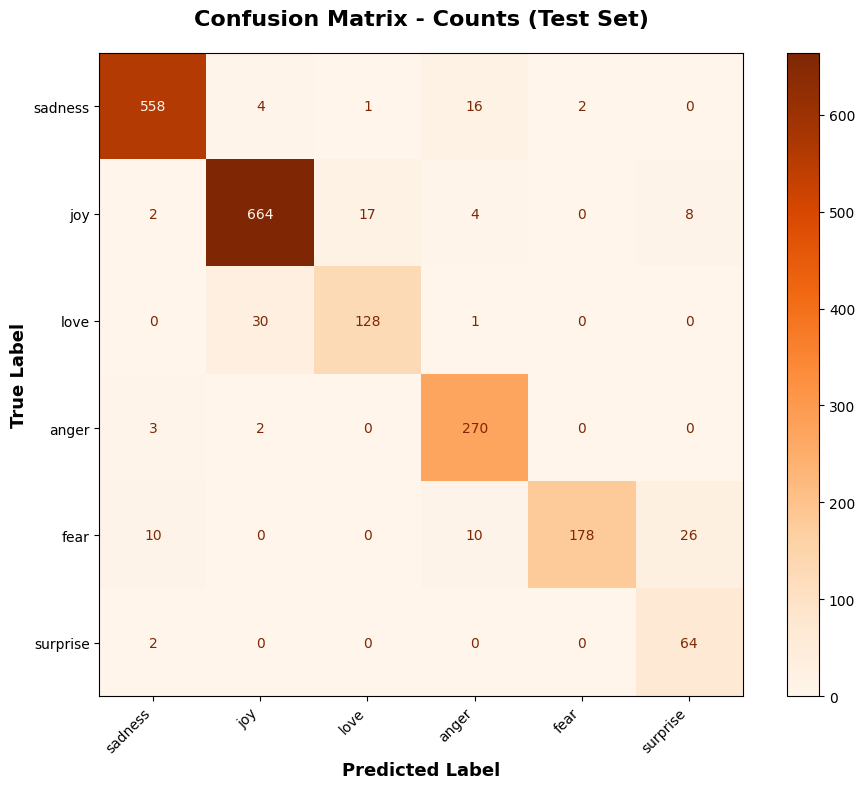
\includegraphics[width=0.75\textwidth]{img/roberta/confusion_matrix_count.png}
    \caption{Matrice di Confusione Quantitativa del modello Full Fine-Tuned.}
    \label{fig:roberta_confusion_matrix_count}
\end{figure}

Di seguito vengono riportati gli errori più comuni con la relativa frequenza registrata:
\begin{table}[H]
    \centering
    \begin{tabular}{|c|c|c|}
        \hline
        \textbf{Vera emozione} & \textbf{Predizione} & \textbf{Frequenza} \\
        \hline
        love                   & joy                 & 30 volte           \\
        fear                   & surprise            & 26 volte           \\
        joy                    & love                & 17 volte           \\
        sadness                & anger               & 16 volte           \\
        fear                   & anger               & 10 volte           \\
        fear                   & sadness             & 10 volte           \\
        joy                    & surprise            & 8 volte            \\
        sadness                & joy                 & 4 volte            \\
        joy                    & anger               & 4 volte            \\
        anger                  & sadness             & 3 volte            \\
        \hline
    \end{tabular}
    \caption{Frequenza degli errori più comuni registrati per RoBERTa-base}
\end{table}


\subsubsection{Risultati Finali e Confronto}
Il seguente grafico riassume i risultati ottenuti dall'applicazione delle diverse strategie di training del modello RoBERTa-base. Si può subito notare come le strategie di Full Fine-Tuning e LoRA abbiano raggiunto risultati nettamente superiori rispetto alle altre strategie. Nel grafico è stata inserita anche la valutazione di RoBERTa-base con la testa di classificazione casuale che a causa dello sbilanciamento delle classi raggiunge un accuracy del $29.05\%$ e un F1 macro del $7.50\%$, rispetto a un accuracy del $16\%$ che si otterrebbe con un dataset bilanciato.

% --- INSERIMENTO DEL GRAFICO QUI ---
\begin{figure}[H]
    \centering
    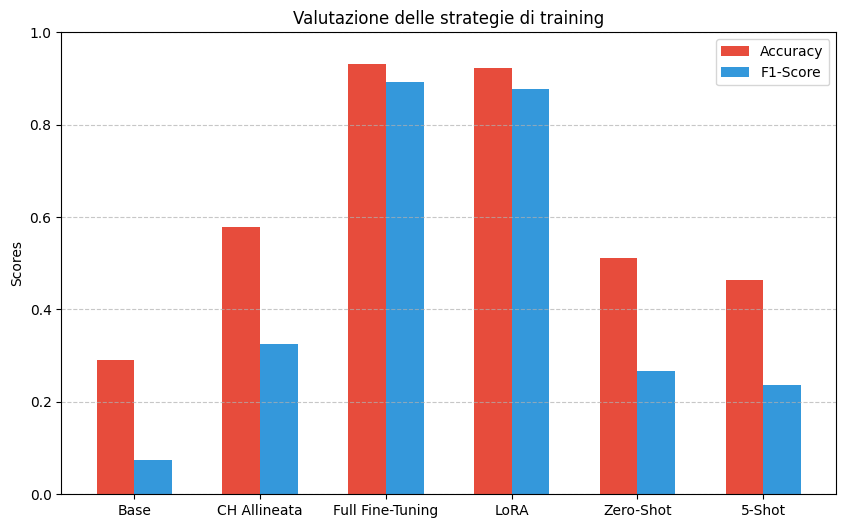
\includegraphics[width=0.85\textwidth]{img/roberta/results.png}
    \caption{Confronto di Accuracy e F1 macro ottenuti tra le diverse strategie testate.}
    \label{fig:roberta_ablation_chart}
\end{figure}
Per conlcudere, di seguito si può trovare una tabella che riassume i migliori risultati per ciascuna strategia utilizzata:

\begin{table}[H]
    \centering
    \renewcommand{\arraystretch}{1.3}
    \begin{tabular}{|l|c|c|p{8cm}|}
        \hline
        \textbf{Strategia}        & \textbf{Accuracy} & \textbf{F1}      & \textbf{Conclusioni}                                                                                        \\
        \hline
        Transfer Learning         & 57.95\%           & 32.50\%          & Performance limitate. Le predizioni si concentrano sulle classi piu frequenti.                              \\
        \hline
        \textbf{Full Fine-Tuning} & \textbf{93.10\%}  & \textbf{89.26\%} & \textbf{Miglior strategia.} L'aggiornamento di tutti i pesi consente al modello di specializzarsi sul task. \\
        \hline
        LoRA                      & 92.35\%           & 87.77\%          & Ottimo compromesso tra efficienza e performance. Ottimo per risorse limitate                                \\
        \hline
        ICL ($0$-Shot)            & 51.15\%           & 26.73\%          & Strategia non adatta a modelli encoder-only.                                                                \\
        \hline
    \end{tabular}
    \caption{Riepilogo finale Ablation Study}
    \label{tab:final_summary}
\end{table}

\subsubsection{Discussione dei Risultati}
Dai risultati ottenuti è facile determinare che, per il task di text emotion classification utilizzando un modello encoder-only come RoBERTa-base, le due strategie più efficienti sono il \textbf{Full Fine-Tuning} e \textbf{LoRA}. Il Full Fine-Tuning risulta la strategia che ha ottenuto risultati migliori, ma con un costo computazionale maggiore dovuto alla richiesta di un elevato numero di risorse per l'aggiornamento del $100\%$ dei parametri. In termini di risorse disponibili, LoRA risulta altamente più efficiente rispetto al Full Fine-Tuning, con un una perdita del $0.75\%$ sul valore di accuracy e del $1.49\%$ sul valore di F1 macro.
I risultati ottenuti sono più che soddisfacenti, in particolare visto lo sbilanciamento delle classi del dataset; con un valore di F1 macro del $89.26\%$ si è dimostrato che il modello risulta in grado di differenziare efficacemente anche le classi meno frequenti come \textbf{suprise} e \textbf{love}.

\subsubsection{Validità del Metodo}
I risultati ottenuto con la strategia di Full Fine-Tuning di RoBERTa-base confermano la validità dell'approccio adottato per il task di \textit{text emotion classification}. Al tempo stesso una strategia come l'ICL mostra come non sia adatta a un modello encoder-only per questo tipo di task.

\subsubsection{Limitazioni e Livello di Maturità}
Il lavoro presenta alcune limitazioni che è opportuno considerare nell'interpretazione dei risultati. Il dataset utilizzato è sbilanciato, di conseguenza, classi come \textit{love} e \textit{fear} sono molto frequenti rispetto ad altre, il che si riflette nel
divario tra accuracy e F1-score macro osservato nelle diverse strategie testate.
Inoltre, l'utilizzo della strategia di ICL, su un modello non adatto, ha fornito risultati che non sono comparabili per un discorso di efficienza rispetto a modelli decoder generativi come GPT, per i quali l'ICL è stato progettato.

\subsubsection{Lavori Futuri}
Il seguente lavoro potrebbe essere esteso con diversi sviluppi futuri.
Un primo contributo significativo sarebbe l'estensione dell'analisi a modelli decoder generativi, come LLaMA o GPT, per una valutazione comparativa dell'efficienza dell'ICL in un contesto architetturale più adeguato. Questo consentirebbe di valutare concretamente il divario di performance rispetto all'approccio encoder-only utilizzato.
Sarebbe, inoltre, interessante estendere l'analisi a modelli multilingua, come XLM-RoBERTa, per valutare lo stesso approccio su testi in lingue diverse dall'inglese e ampliare il campo di applicazione del sistema sviluppato.

\section{Confronto Finale tra i Modelli}

In questa sezione vengono messi a confronto i risultati ottenuti dai quattro modelli analizzati:
\texttt{vinai/bertweet-base}, \texttt{distilbert-base-uncased}, \texttt{bert-base-uncased} e \texttt{FacebookAI/roberta-base}.
Il confronto è strutturato per strategia di training, al fine di isolare l'impatto dell'architettura del modello
a parità di approccio.

\subsection{Confronto per Strategia}

\subsubsection{In-Context Learning}

\begin{table}[H]
    \centering
    \renewcommand{\arraystretch}{1.3}
    \begin{tabular}{|l|c|c|c|}
        \hline
        \textbf{Modello}                 & \textbf{Shots} & \textbf{Accuracy} & \textbf{F1 Macro} \\
        \hline
        \texttt{bert-base-uncased}       & 1 & \textbf{48.90\%}  & \textbf{20.35\%}  \\
        \texttt{distilbert-base-uncased} & 1 & 48.05\%           & 25.63\%           \\
        \texttt{bertweet-base}           & 1 & 46.87\%           & 22.28\%           \\
        \texttt{roberta-base}            & 1 & 43.53\%           & 21.22\%           \\
        \hline
    \end{tabular}
    \caption{Confronto In-Context Learning (1-Shot) tra i modelli}
\end{table}

In tutti i modelli l'ICL produce risultati contenuti, coerentemente con la natura encoder-only delle architetture analizzate: questi modelli non sono stati progettati per il condizionamento del contesto tipico dell'ICL, che risulta invece un punto di forza dei modelli decoder generativi. 

\begin{table}[H]
    \centering
    \renewcommand{\arraystretch}{1.3}
    \begin{tabular}{|l|c|c|c|}
        \hline
        \textbf{Modello}                 & \textbf{Shots} & \textbf{Accuracy} & \textbf{F1 Macro} \\
        \hline
        \texttt{roberta-base}            & 0 & \textbf{51.15\%}  & \textbf{26.73\%}  \\
        \texttt{bertweet-base}           & 0 & 49.30\%           & 24.63\%           \\
        \hline
    \end{tabular}
    \caption{Confronto In-Context Learning (0-Shot) tra i modelli}
\end{table}

Si può notare come la configurazione zero-shot, testata sui modelli RoBERTa-base e BERTweet, ottenga risultati migliori rispetto alla configurazione 1-shot, suggerendo che l'aggiunta di esempi nel contesto possa interferire con il pattern del prompt atteso dal Masked Language Modeling (MLM) e degradare le performance.

\subsubsection{Fine-tuning Completo}

\begin{table}[H]
    \centering
    \renewcommand{\arraystretch}{1.3}
    \begin{tabular}{|l|c|c|l|}
        \hline
        \textbf{Modello}                 & \textbf{Accuracy} & \textbf{F1 Macro} & \textbf{Note}                    \\
        \hline
        \texttt{bertweet-base}           & \textbf{93.40\%}  & \textbf{89.90\%}  & Domain-specific su Twitter.      \\
        \texttt{roberta-base}            & 93.10\%           & 89.26\%           & Stabile su tutto il range di LR. \\
        \texttt{bert-base-uncased}       & 93.00\%           & 87.72\%           & Early stopping all'epoca 2.00.   \\
        \texttt{distilbert-base-uncased} & 92.60\%           & 87.61\%           & Early stopping all'epoca 1.75.   \\
        \hline
    \end{tabular}
    \caption{Confronto Full Fine Tuning tra i modelli}
\end{table}

Il Full Fine Tuning produce risultati molto simili tra tutti i modelli, con accuracy compresa tra 92.60\% e 93.40\%.
BERTweet ottiene il margine migliore, probabilmente grazie al pre-training su dati Twitter, semanticamente
più vicini al dataset di riferimento. È degno di nota che DistilBERT, pur avendo la metà dei parametri di BERT,
raggiunge prestazioni competitive, dimostrando una buona efficienza parametrica.

\subsubsection{[Extra] Transfer Learning (Frozen)}

\begin{table}[H]
    \centering
    \renewcommand{\arraystretch}{1.3}
    \begin{tabular}{|l|c|c|}
        \hline
        \textbf{Modello}       & \textbf{Accuracy} & \textbf{F1 Macro} \\
        \hline
        \texttt{roberta-base}  & \textbf{57.95\%}  & \textbf{32.50\%}  \\
        \texttt{bertweet-base} & 54.15\%           & 29.62\%           \\
        \hline
    \end{tabular}
    \caption{Confronto Transfer Learning (Frozen) tra i modelli}
\end{table}

In questa configurazione tutti i modelli mostrano prestazioni limitate, con accuracy massima attorno al 58\%.
RoBERTa ottiene l'accuracy più alta, ma nessun modello supera il 60\%, confermando che il semplice allineamento
della testa di classificazione è insufficiente per un task emotivo articolato come questo.

\subsubsection{[Extra] LoRA }

\begin{table}[H]
    \centering
    \renewcommand{\arraystretch}{1.3}
    \begin{tabular}{|l|c|c|l|}
        \hline
        \textbf{Modello}       & \textbf{Accuracy} & \textbf{F1 Macro} & \textbf{Configurazione Ottimale}             \\
        \hline
        \texttt{bertweet-base} & \textbf{93.20\%}  & \textbf{89.10\%}  & $r=16$, \texttt{[q,v,k,dense]}, $LR=2e^{-4}$ \\
        \texttt{roberta-base}  & 92.65\%           & 88.46\%           & $r=32$, $LR=5e^{-4}$, $BS=16$                \\
        \hline
    \end{tabular}
    \caption{Confronto LoRA tra i modelli (solo modelli per cui è stata applicata)}
\end{table}

\subsection{Sintesi Finale}

\begin{table}[H]
    \centering
    \renewcommand{\arraystretch}{1.3}
    \begin{tabular}{|l|c|c|c|}
        \hline
        \textbf{Modello}                 & \textbf{Parametri} & \textbf{Best Accuracy} & \textbf{Best F1 Macro} \\
        \hline
        \texttt{bertweet-base}           & 134M               & \textbf{93.40\%}       & \textbf{89.90\%}       \\
        \texttt{roberta-base}            & 124M               & 93.10\%                & 89.26\%                \\
        \texttt{bert-base-uncased}       & 110M               & 93.00\%                & 87.72\%                \\
        \texttt{distilbert-base-uncased} & 66M                & 92.60\%                & 87.61\%                \\
        \hline
    \end{tabular}
    \caption{Riepilogo dei migliori risultati ottenuti per ciascun modello (Full Fine Tuning)}
    \label{tab:model_comparison}
\end{table}

I risultati evidenziano che, a parità di strategia di training ottimale (Full Fine Tuning), le differenze
prestazionali tra i modelli sono contenute (meno dell'1\% di accuracy), suggerendo che la strategia di
addestramento ha un impatto maggiore rispetto alla scelta dell'architettura in questo task.
BERTweet si conferma la scelta migliore grazie alla specializzazione sul dominio Twitter, ma la sua superiorità
è marginale rispetto a modelli general-purpose come RoBERTa e BERT.
DistilBERT rappresenta la scelta più efficiente in termini di rapporto prestazioni/parametri,
raggiungendo il 92.60\% con soli 66M di parametri, circa la metà degli altri modelli analizzati.

\subsection{Limitazioni e Livello di Maturità}
\begin{itemize}
    \item \textbf{Limiti:} La \textit{Context Window} limitata impedisce l'uso di prompt complessi o catene di ragionamento.
          Il dataset presenta un sbilanciamento naturale che penalizza leggermente le classi minoritarie (\textit{Surprise}).
    \item \textbf{Maturità:} La soluzione sviluppata, basata su librerie standard industriali (\texttt{transformers}, \texttt{peft}),
          ha raggiunto un buon livello di maturità tecnologica, pronta per essere integrata in pipeline di produzione con costi
          di inferenza contenuti.
\end{itemize}

\subsection{Lavori Futuri}
Per avanzare ulteriormente nel progetto e superare i limiti identificati, proponiamo le seguenti direzioni di ricerca:

\begin{enumerate}
    \item \textbf{Data Augmentation via Back-Translation:} Per mitigare lo sbilanciamento delle classi (in particolare \textit{Surprise}, che ha pochi campioni), proponiamo di generare dati sintetici utilizzando una pipeline di traduzione andata-ritorno (es. Inglese $\rightarrow$ Francese $\rightarrow$ Inglese). Questa tecnica introduce variazioni lessicali e sintattiche naturali mantenendo inalterata la semantica originale, arricchendo il training set con esempi diversificati che rendono il modello più robusto sulle classi minoritarie.

    \item \textbf{Supervised Contrastive Learning:} Per risolvere l'ambiguità tra classi semanticamente sovrapposte come \textit{Love} e \textit{Joy}, suggeriamo di introdurre una fase preliminare di addestramento con \textit{SupCon Loss}. A differenza della classica Cross-Entropy (che valuta i campioni singolarmente), la loss contrastiva lavora su coppie: forza l'encoder ad avvicinare drasticamente le rappresentazioni vettoriali dei tweet della stessa classe e ad allontanare quelle di classi diverse nello spazio latente. Questo creerebbe confini decisionali più netti prima ancora di addestrare il classificatore finale.

    \item \textbf{Task-Adaptive Pre-Training:} Invece di passare direttamente dal modello generico (\texttt{BERTweet}) al fine-tuning, proponiamo una fase intermedia di "riscaldamento". Questa consiste nel continuare il pre-training con obiettivo \textit{Masked Language Modeling} (MLM) utilizzando i soli testi del dataset \texttt{emotion} (senza etichette). Questo adatta i pesi dell'encoder allo specifico vocabolario, slang e distribuzione linguistica del nostro dataset, ottimizzando la capacità del modello di estrarre feature rilevanti da contesti emotivi ambigui prima di applicare LoRA.
\end{enumerate}

% --- BIBLIOGRAPHY ---
\newpage
\printbibliography[title={References}]

\end{document}
